\documentclass[11pt]{article}

\usepackage[margin=1in]{geometry}
\usepackage{amsmath,amssymb}
\usepackage{booktabs}
\usepackage{graphicx}
\usepackage{multirow}
\usepackage{xcolor}
\usepackage{microtype}
\usepackage[numbers,sort&compress]{natbib}
\usepackage[font=small,labelfont=bf]{caption}
\PassOptionsToPackage{hyphens}{url}
\usepackage[colorlinks=true,linkcolor=blue!50!black,citecolor=blue!50!black,urlcolor=blue!50!black]{hyperref}
\Urlmuskip=0mu plus 1mu\relax
\emergencystretch=1.2em
\renewcommand{\bibfont}{\footnotesize}
\usepackage{enumitem}
\setlist{itemsep=2pt, topsep=3pt, parsep=0pt}
\usepackage[compact]{titlesec}
\setlength{\textfloatsep}{14pt plus 2pt minus 4pt}

% ---------------------------------------------------------------------------
%
% file to switch: the dark targets \def\DARKMODE{} before \documentclass[11pt]{article}

\usepackage[margin=1in]{geometry}
\usepackage{amsmath,amssymb}
\usepackage{booktabs}
\usepackage{graphicx}
\usepackage{multirow}
\usepackage{xcolor}
\usepackage{microtype}
\usepackage[numbers,sort&compress]{natbib}
\usepackage[font=small,labelfont=bf]{caption}
\PassOptionsToPackage{hyphens}{url}
\usepackage[colorlinks=true,linkcolor=blue!50!black,citecolor=blue!50!black,urlcolor=blue!50!black]{hyperref}
\Urlmuskip=0mu plus 1mu\relax
\emergencystretch=1.2em
\renewcommand{\bibfont}{\footnotesize}
\usepackage{enumitem}
\setlist{itemsep=2pt, topsep=3pt, parsep=0pt}
\usepackage[compact]{titlesec}
\setlength{\textfloatsep}{14pt plus 2pt minus 4pt}

% ---------------------------------------------------------------------------
%
% file to switch: the dark targets \def\DARKMODE{} before \documentclass[11pt]{article}

\usepackage[margin=1in]{geometry}
\usepackage{amsmath,amssymb}
\usepackage{booktabs}
\usepackage{graphicx}
\usepackage{multirow}
\usepackage{xcolor}
\usepackage{microtype}
\usepackage[numbers,sort&compress]{natbib}
\usepackage[font=small,labelfont=bf]{caption}
\PassOptionsToPackage{hyphens}{url}
\usepackage[colorlinks=true,linkcolor=blue!50!black,citecolor=blue!50!black,urlcolor=blue!50!black]{hyperref}
\Urlmuskip=0mu plus 1mu\relax
\emergencystretch=1.2em
\renewcommand{\bibfont}{\footnotesize}
\usepackage{enumitem}
\setlist{itemsep=2pt, topsep=3pt, parsep=0pt}
\usepackage[compact]{titlesec}
\setlength{\textfloatsep}{14pt plus 2pt minus 4pt}

% ---------------------------------------------------------------------------
%
% file to switch: the dark targets \def\DARKMODE{} before \documentclass[11pt]{article}

\usepackage[margin=1in]{geometry}
\usepackage{amsmath,amssymb}
\usepackage{booktabs}
\usepackage{graphicx}
\usepackage{multirow}
\usepackage{xcolor}
\usepackage{microtype}
\usepackage[numbers,sort&compress]{natbib}
\usepackage[font=small,labelfont=bf]{caption}
\PassOptionsToPackage{hyphens}{url}
\usepackage[colorlinks=true,linkcolor=blue!50!black,citecolor=blue!50!black,urlcolor=blue!50!black]{hyperref}
\Urlmuskip=0mu plus 1mu\relax
\emergencystretch=1.2em
\renewcommand{\bibfont}{\footnotesize}
\usepackage{enumitem}
\setlist{itemsep=2pt, topsep=3pt, parsep=0pt}
\usepackage[compact]{titlesec}
\setlength{\textfloatsep}{14pt plus 2pt minus 4pt}

% ---------------------------------------------------------------------------
%
% file to switch: the dark targets \def\DARKMODE{} before \input{main.tex}.
% When ON: near-black blue-warm page, light-gray body text (never pure white,
% to avoid halation), brighter section heads, soft cyan/amber links, salmon
% figures/dark/ (generated by scripts/make_figures.py --dark).
\newif\ifdarkmode
\ifdefined\DARKMODE
  \darkmodetrue
\else
  \darkmodefalse
\fi

\ifdarkmode
  % Visual definitions shared with explainer.tex (pure extraction, no
  % behavior change): colors, \pagecolor, default-color patch, \hypersetup,
  % bright section heads.
  \input{darkstyle}
  \graphicspath{{figures/dark/}}
\else
  \graphicspath{{figures/}}
\fi
% ---------------------------------------------------------------------------


% Quant names appear constantly; keep them readable.
\newcommand{\q}[1]{\texttt{#1}}
\newcommand{\singleauthorinfo}[1]{\\[0.25em]{\small #1}}

\title{\textbf{Deploying Qwen3.8-27B in 12\,GB of VRAM: Accuracy and
Throughput Across Quantized Inference Stacks}}

\hypersetup{
  pdftitle={Deploying Qwen3.8-27B in 12 GB of VRAM: Accuracy and Throughput Across Quantized Inference Stacks},
  pdfauthor={Matthew Schwartz},
  pdfsubject={Quantized large-language-model inference under a 12 GB GPU memory budget}
}

\author{Matthew Schwartz\singleauthorinfo{Independent researcher \enspace
\href{https://orcid.org/0009-0009-4171-7247}{ORCID 0009-0009-4171-7247}
\enspace \texttt{matthew.schwartz.research@gmail.com}}}

\date{August 29, 2026}

\begin{document}
\maketitle

\begin{abstract}
\noindent
Quantized-inference studies usually report quality under a fixed engine or
throughput under a fixed quantization, but a 12\,GB GPU couples these choices:
weights, cache, and engine buffers must fit together, and spilled weights are
read from slower system RAM. We characterize this deployment problem for
Qwen3.8-27B on an 80\,W RTX 4080 Laptop GPU by measuring fit, throughput, and
task performance for eight artifacts across GGUF/llama.cpp and
EXL3/ExLlamaV3. Fully resident GGUFs decoded at 24.4--25.5 tokens/s, whereas
partial offload reduced decode to 16.6--4.9 tokens/s. At approximately
9.5\,GiB file footprint, EXL3/ExLlamaV3 remained fully resident while
GGUF/llama.cpp offloaded six of 65 units; the hard-suite samples did not
resolve an accuracy difference, but EXL3 generated $1.6\times$ faster on MATH
and achieved the highest observed correct responses per minute on MATH and
HumanEval+. Across GGUF, the 2.16-effective-bpw artifact lost seven paired
MATH items relative to the 2.49-effective-bpw artifact, while configurations
from 2.49 to 5.22 effective bpw were not separated at these sample sizes; the
original MATH parser also disagreed with the post-hoc normalizer unevenly
across artifacts, so we report both scores separately. On this machine, joint
artifact--engine selection kept a 27.4B model in 12\,GB of VRAM and delivered
correct responses faster than partial offload, with no hard-task difference
resolved relative to the largest tested artifact; we did not test bf16 or Q8,
or isolate engine from format.
\end{abstract}



\section{Introduction}
\label{sec:intro}

Quantized-inference work usually reports either quality under a fixed engine or
throughput under a fixed quantization. A 12\,GB discrete GPU couples the two:
the file, cache, and engine buffers must fit together, and crossing that boundary
moves weight reads from high-bandwidth VRAM to much slower system RAM. The
practical question is therefore not simply ``which quant has the best quality?''
It is: \emph{which artifact--engine pair returns correct answers fastest inside
this fixed memory budget?}

We answer that question for Qwen3.8-27B, whose 27.36 billion non-MTP VLM
parameters would require roughly 54.7\,GB at bf16 before runtime overhead, on
one 12\,GB laptop GPU. In
the measured run state, the right low-bit artifact and engine kept the model
fully GPU-resident. Its scores on the small hard-task suites were not resolved
from those of the largest tested artifact, and it returned more correct answers
per minute than the larger deployments that placed weights in system RAM. This
is the paper's central result: the machine did more useful work with a smaller,
fully resident deployment than with the largest tested, partially offloaded
artifact, which kept only 33 of 65 offload units on the GPU. More useful work
here means more correctly scored responses per minute, not a resolved
raw-accuracy advantage.

We first found the maximum GPU-resident layer count and measured prompt and
decode throughput for a GGUF ladder. We then evaluated selected configurations
on easy and harder task subsets, inspected MATH scoring failures item by item,
added a GGUF control with nearly the same file footprint as EXL3, and compared
the two recommended deployments on MMLU and long-context probes. We report
nominal quantization, actual checkpoint size, GPU residency, task score, and
wall-clock response rate separately.

\paragraph{Contribution and scope.}
The primary contribution is an end-to-end deployment map for a 27.4B model
under a 12\,GB laptop-GPU memory budget. It connects checkpoint footprint and
engine-specific residency to controlled throughput, benchmark accuracy, and
correct responses per minute. Fully resident GGUFs decoded at 24--25 tokens/s,
whereas progressively offloaded GGUFs fell to 16.6--4.9 tokens/s. At matched
file footprint, EXL3/ExLlamaV3 remained resident and generated faster than
GGUF/llama.cpp without a resolved hard-suite score difference.

Two audits qualify that result. Nominal bit labels did not reliably predict
whole-checkpoint size, and the post-hoc MATH normalizer accepted some surface
forms that the original parser rejected. We therefore compare complete artifact--engine
deployments rather than attributing the cross-stack result to trellis coding,
and report the original-parser score beside a disclosed post-hoc-normalized
score. The latter is a rescore of saved outputs, not an independent semantic
ground truth.

The hard-suite subsets are small ($n{=}20$--$25$), every generation is a single
sample at temperature 1.0, and engine and format cannot be separated in the
cross-ecosystem comparison. Wilson 95\% intervals accompany every accuracy.
These data characterize the tested deployments; they do not establish model-
or hardware-class generalities (\S\ref{sec:limitations}).


\section{Experimental Setup}
\label{sec:setup}

\subsection{Hardware}
\label{sec:hw}

All measurements were taken on a single consumer laptop: NVIDIA GeForce RTX
4080 Laptop GPU (Ada Lovelace, SM~8.9), 12{,}282\,MiB VRAM, capped at
\textbf{80\,W}; Intel Core i9-14900HX CPU; 62\,GiB dual-channel DDR5; NVMe
storage; Linux 7.0.0, driver 580.167.08. The desktop session held
$\sim$900\,MiB of VRAM, leaving a measured working envelope of roughly
10.5--11\,GiB for weights, cache/state, and compute buffers. Power mode, memory
clock, and sustained device clocks were not separately logged; the throughput
results therefore describe this run state, not a normalized hardware limit.

Batch-one dense decode is usually memory-bandwidth-bound: each generated
token's forward pass uses the active weight set, which is too large to remain
in on-chip cache, so memory traffic scales approximately with active weight
bytes and $\text{tok/s} \approx
\text{effective bandwidth}/\text{bytes per token}$. The laptop's GDDR6 is
$\sim$432\,GB/s on paper; our fitted effective GPU-resident weight-path
bandwidth is 199\,GB/s (\S\ref{sec:offload}). The fitted CPU-resident
weight-path coefficient is 41\,GB/s---roughly $5\times$ lower. It absorbs
memory-transfer and decode effects and is not a raw DDR5 specification. This
two-bandwidth model is descriptive of the observed GGUF ladder;
quant-family-specific CPU kernels account for its largest residuals.


\subsection{Model}
\label{sec:model}

Qwen3.8-27B (released 2026-08-14) is an instruction-tuned vision--language
model with 26.896B main-language parameters and 0.461B vision parameters
(27.36B non-MTP parameters, rounded to 27.4B here). Its separate MTP head has
0.425B parameters. The model card reports a
\emph{hybrid} sequence mixer: only 16 of 64 layers are classical attention
with a growing KV cache (4~KV heads $\times$ 256 head dim), while the other 48
are DeltaNet-style linear-attention layers \citep{qwen38model}. Gated Delta
Networks and Mamba provide the architectural background
\citep{yang2024gateddeltanet,gu2023mamba}; the recurrent layers hold a
constant-size state ($\sim$150\,MB total here). Verified KV cost is
$2 \times 4 \times 256 \times 2\,\text{B} \times 16 = \mathbf{64\,KiB/token}$
at fp16 ($\sim$38\,KiB at q8\_0) --- $4\times$ lower than a counterfactual
64-layer model using the same four-KV-head attention block in every layer. At
the tested context lengths, KV-memory growth was therefore
relatively cheap and \emph{fitting was primarily a weights problem}. The
release ecosystem also provides a 1.28\,GiB multi-token-prediction (MTP) head;
the tested llama.cpp build used it as an in-model draft
\citep{qwen38model,gerganov2023llamacpp}, an instance of speculative decoding
\citep{leviathan2022speculative,chen2023speculative}. It also provides a
0.86\,GiB vision
projector (vision was not evaluated). These components are packaged
differently: the unsloth GGUF release stores both separately, the bartowski
GGUF embeds the MTP tensors, and the tested EXL3 checkpoint has no configured
draft or vision path. The 248K-token vocabulary makes the text embeddings a
large, hard-to-quantize fraction of every weight artifact --- one reason
nominal and effective bits-per-weight diverge (Table~\ref{tab:artifacts}).


\subsection{Engines}
\label{sec:engines}

Two inference stacks: \textbf{llama.cpp} \citep{gerganov2023llamacpp} built
from master at \q{b1-1729ed5} with a user-local CUDA 12.6.3 toolchain
(SM~8.9), serving GGUF artifacts with layer-wise CPU offload (\q{-ngl}); and
\textbf{ExLlamaV3 1.4.3} \citep{turboderp2025exllamav3} via TabbyAPI, serving
EXL3 trellis-quantized safetensors. For this tested dense checkpoint, the stack
used no supported dense-layer CPU weight-offload path, so the complete model
had to fit in VRAM. Unless noted:
context 8192, KV cache q8\_0, flash attention on, the model card's recommended
thinking-mode sampling (temperature 1.0, top-p 0.95, top-k 20)
\citep{qwen38model}, and the chat template's
\q{reasoning\_effort} set to \emph{medium}.


\subsection{Artifacts}
\label{sec:artifacts}

Table~\ref{tab:artifacts} lists the eight evaluated weight artifacts with their
measured checkpoint weight-file total and \emph{effective} bits per weight,
computed as $8B/26{,}895{,}998{,}464$ for total weight-file bytes $B$ and the
exact main-language parameter count. We report effective bpw beside every
nominal label throughout the paper; the two diverge by up to 52\% and the
difference determines which artifacts are valid footprint controls in
\S\ref{sec:exl3}.

\begin{table}[t]
\centering
\small
\caption{Eight evaluated weight artifacts. Effective bpw
$=8B/26{,}895{,}998{,}464$ for checkpoint weight-file total $B$, normalized
by the exact main-language parameter count; it can exceed the nominal label because embeddings
(248K vocabulary), norms, and (for EXL3) the 3-bit head quantize wider than the
label. Downloaded 2026-08-25 from \q{unsloth/Qwen3.8-27B-GGUF},
\q{bartowski/Qwen3.8-27B-GGUF}, and turboderp's EXL3 conversions
(\q{SC\_2.00bpw\_H3}). The optional unsloth MTP draft is listed separately and
is not included in its target file size.}
\label{tab:artifacts}
\setlength{\tabcolsep}{4pt}
\begin{tabular}{llrrl}
\toprule
Artifact & Format & File & Eff.\ bpw & Note \\
\midrule
\q{UD-IQ2\_XXS} & GGUF i-quant, unsloth UD & 6.77\,GiB & 2.16 & smallest under test \\
\q{UD-IQ2\_S} & GGUF i-quant, unsloth UD & 7.80\,GiB & 2.49 & largest full-GPU fit \\
\q{UD-Q2\_K\_XL} & GGUF k-quant, unsloth UD & 9.15\,GiB & 2.92 & \\
\q{IQ2\_S} (bartowski) & GGUF i-quant & 9.59\,GiB & 3.06$^{a}$ & MTP head baked in \\
\q{UD-IQ3\_XXS} & GGUF i-quant, unsloth UD & 10.18\,GiB & 3.25 & \\
\q{UD-IQ3\_S} & GGUF i-quant, unsloth UD & 11.21\,GiB & 3.58 & \\
\q{UD-Q4\_K\_XL} & GGUF k-quant, unsloth UD & 16.35\,GiB & 5.22 & largest quality anchor \\
EXL3 2.0\,bpw & EXL3 trellis (QTIP-style) & 9.50\,GiB & 3.03 & nominal 2.0; head at 3\,bpw \\
\midrule
Optional MTP draft & GGUF Q4\_0 & 1.28\,GiB & --- & separate for unsloth targets \\
\bottomrule
\multicolumn{5}{l}{\footnotesize $^{a}$Includes the baked-in MTP head, so main-model bpw is lower.}
\end{tabular}
\end{table}


\subsection{Evaluation Protocol and Metrics}
\label{sec:harness}

The fit-and-throughput campaign used a guarded harness (never launch unless estimated VRAM $\leq$
free$-$500\,MiB and available RAM covers CPU-resident bytes $+8$\,GiB; weights
always mmap-backed) that runs, per artifact: a fit search for the maximum
GPU-resident layer count at ctx 8192, \q{llama-bench} pp512/tg128 at that fit,
and timed \q{llama-server} generations (prose and code prompts, MTP off/on).
llama.cpp reports 65 offload units for this 64-block model because its count
includes the output layer. Each result is written and flushed to JSONL
immediately.

The accuracy campaign evaluated served models through the OpenAI-compatible endpoint on four
suites: \textbf{GSM8K} \citep{cobbe2021gsm8k} $\times 50$, strict answer
extraction; \textbf{HumanEval} \citep{chen2021humaneval} $\times 20$, generated
code executed against the official tests; \textbf{MATH-25}: 25 competition
problems at MATH levels 4--5 \citep{hendrycks2021math}, 8K-token generation
budget, truncations scored wrong; and \textbf{HumanEval+} $\times 20$
\citep{liu2023evalplus}, execution against EvalPlus's $\sim$80$\times$
augmented test sets. Every accuracy in this paper carries a Wilson 95\%
interval in brackets. The subsets were sampled deterministically with seed 42;
MATH-25 was stratified across all seven subjects, and HumanEval+ used the same
20 problems as HumanEval. A final validation compared the two selected
deployments on a 200-item, 57-subject-stratified MMLU subset
\citep{hendrycks2021mmlu} and six synthetic
needle contexts (8K/16K/32K, two insertion depths). For MATH, the
\emph{original-parser score} applies the answer extractor and acceptance rules
used during the run. The \emph{post-hoc-normalized score} applies a disclosed,
deterministic normalizer to the same saved responses; it does not regenerate
answers and is not an independent judgment of semantic correctness. At
$n{=}20$--$25$ the
intervals are wide. They reflect item sampling, not the additional variation
from single stochastic generations.



\section{Results}
\label{sec:phase1}

\subsection{GPU Residency and Throughput}

\begin{table}[t]
\centering
\footnotesize
\setlength{\tabcolsep}{3.5pt}
\caption{Controlled GGUF speed matrix (llama.cpp \q{b1-1729ed5}; ctx 8192,
KV q8\_0, flash-attn on; desktop session running). tg = \q{llama-bench} tg128;
server-measured decode agreed within $\pm 0.4$\,tok/s. EXL3 is excluded because
no matching \q{tg128} measurement was collected; its workload measurements are
reported separately in \S\ref{sec:exl3}.}
\label{tab:phase1}
\begin{tabular}{lrrrrrl}
\toprule
Config & File & GPU layers & tg tok/s & pp512 & VRAM peak & MTP effect on tg \\
\midrule
\q{UD-IQ2\_XXS} & 6.8\,GiB & \textbf{65/65} & \textbf{25.5} & 733 & 8.6--8.9\,GiB & $+21\%\rightarrow$ 30.9 (GPU draft); \\
 & & & & & & \quad 48--50 math; $-16\%$ CPU draft \\
\q{UD-IQ2\_S} & 7.8\,GiB & \textbf{65/65} & \textbf{24.4} & 708 & 9.7--10.0\,GiB & draft misses fit by $\sim$100\,MiB \\
\q{UD-Q2\_K\_XL} & 9.2\,GiB & 61/65 & 16.6 & 652 & 10.0--10.4\,GiB & crashed (draft buffers, see text) \\
\q{IQ2\_S} (bartowski) & 9.6\,GiB & 59/65 & 13.8 & 580 & 9.5--10.2\,GiB & not tested \\
\q{UD-IQ3\_XXS} & 10.2\,GiB & 54/65 & 11.3 & 608 & 10.4--10.8\,GiB & crashed (draft buffers) \\
\q{UD-IQ3\_S} & 11.2\,GiB & 49/65 & 8.2 & 559 & 10.5--10.7\,GiB & crashed (draft buffers) \\
\q{UD-Q4\_K\_XL} & 16.4\,GiB & 33/65 & 4.9 & 361 & 10.5\,GiB & wash ($+8\%$ prose, $-8\%$ code) \\
\emph{CPU floor} (\q{UD-IQ2\_S}) & 7.8\,GiB & 0/65 & 3.3 & 4.1 & --- & --- \\
\bottomrule
\end{tabular}
\end{table}

\begin{figure}[t]
\centering
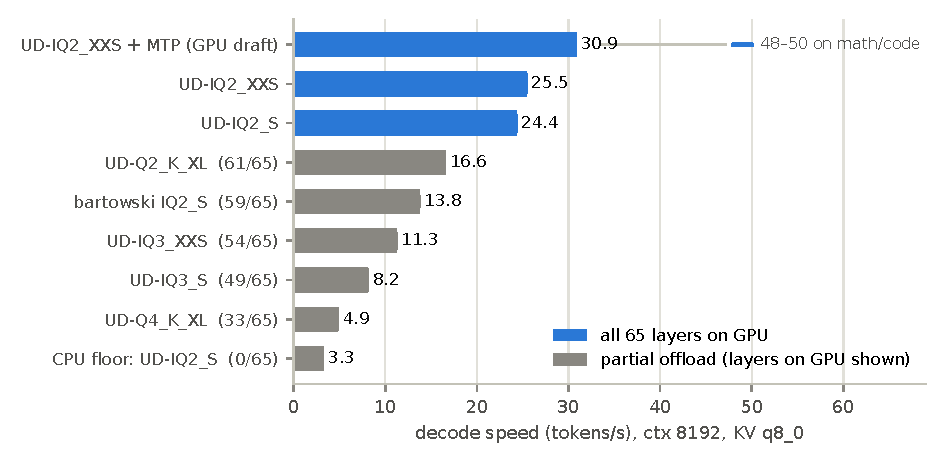
\includegraphics[width=\textwidth]{fig_ladder.pdf}
\caption{The measured speed ladder. Blue: all 65 layers GPU-resident; gray:
partial offload (GPU layer count in the label). The \q{UD-IQ2\_XXS}+MTP bar
shows prose decode; the whisker marks its measured 48--50\,tok/s on
math/code content (\S\ref{sec:mtp}). All base bars use the same
\q{llama-bench} tg128 protocol; the MTP annotations are separate server
measurements.}
\label{fig:ladder}
\end{figure}

Table~\ref{tab:phase1} and Figure~\ref{fig:ladder} give the matrix. The
full-residency boundary is the dominant feature; nominal labels and prompt
processing add two important qualifications.

\paragraph{For llama.cpp/GGUF, the full-GPU boundary lies between 7.8 and
9.2\,GiB in this run state.}
With the desktop session holding $\sim$900\,MiB, only the 6.8 and 7.8\,GiB
artifacts fit all 65 layers. Everything larger sheds layers to system RAM and
slows immediately. Within the GGUF ladder, footprint and consequent residency
are the first-order predictors of speed. This boundary is engine-specific:
ExLlamaV3 later fits a 9.50\,GiB EXL3 checkpoint (\S\ref{sec:exl3}).

\paragraph{The nominal quant label does not determine footprint or speed.}
Unsloth's \q{UD-IQ2\_S} (7.8\,GiB, 2.49 effective bpw) runs 24.4\,tok/s;
bartowski's \q{IQ2\_S} (9.6\,GiB, 3.06 effective bpw) runs 13.8\,tok/s. The
files share a nominal label but not a size, tensor allocation, or packaging:
the bartowski file also embeds MTP tensors. The observed speed difference is
consistent with full versus partial residency; it does not isolate a
quant-maker or allocation effect.

\paragraph{At 512 prompt tokens, GPU-heavy configurations ingest much faster
than they decode.} The controlled pp512 rates were 360--733\,tok/s, while the
CPU-only i-quant floor fell to 4.1\,tok/s. These short-context microbenchmarks
must not be extrapolated to 32K prompts; the deadline behavior in
\S\ref{sec:exl3} shows why.


\subsection{Offload Decay Follows a Two-Bandwidth Model}
\label{sec:offload}

\begin{figure}[t]
\centering
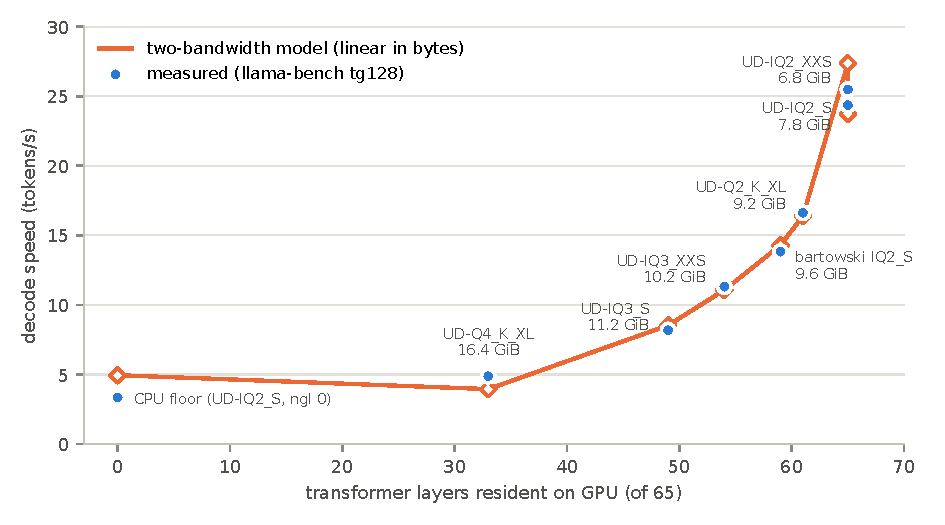
\includegraphics[width=\textwidth]{fig_offload.pdf}
\caption{Decode speed vs.\ GPU-resident layer count (blue, measured), with the
two-bandwidth model's per-config predictions (orange). The model, fitted for
relative error over all eight points, is
$1/\text{tok/s} = b_{\text{GPU}}/199\,\text{GB/s} +
b_{\text{CPU}}/41\,\text{GB/s}$ where $b$ are resident byte counts
(file bytes split proportionally to layers). The six non-extreme measured
states land within $\pm 8\%$; the two extremes' deviations are consistent with a
quant-family-dependent CPU term (i-quants dequantize expensively on CPU, so the ngl-0
floor runs $32\%$ below the pure-bandwidth prediction, while k-quant
\q{UD-Q4\_K\_XL} runs $24\%$ above it).}
\label{fig:offload}
\end{figure}

Figure~\ref{fig:offload} tests the bandwidth model of \S\ref{sec:hw} against
the matrix. Per-token time is linear in the two resident byte counts, with
fitted effective path bandwidths of \textbf{199\,GB/s} (GPU-resident bytes)
and \textbf{41\,GB/s} (CPU-resident bytes) --- a $4.9\times$ ratio, and the
reason each shed layer costs so much.
The fit's residual structure is itself informative: deviations concentrate
where CPU dequantization cost differs by quant family, i.e., the ``linear in
bytes'' rule needs a per-family CPU coefficient before it can be used
predictively across formats. For ranking configs on one family it is already
accurate to a few percent.


\subsection{MTP Benefit Depends on Workload and Placement}
\label{sec:mtp}

On the controlled prose prompt, the MTP draft head increased decode throughput by
21\% (25.5 $\rightarrow$ 30.9\,tok/s) at temperature 1.0 with the draft fully
on GPU, at a 41\% acceptance rate. During the MATH run, the same deployed
configuration produced 45--50 output tokens/s. That higher workload rate is
consistent with greater acceptance on structured text, but no draft-off run was
collected on the identical MATH prompts, so it is not a controlled 90\% MTP
effect. Likewise, the 9.6\,s mean GSM8K item time for
\q{UD-IQ2\_XXS}+MTP versus 17.7\,s for \q{UD-IQ2\_S} is a deployment
comparison, not an isolated MTP comparison: both the artifact and draft setting
change.

Two operational caveats. First, with the draft on CPU, MTP was a \emph{loss}
($-16\%$) or a wash in the controlled prose runs; these results should not be carried
over to other sampling regimes. Second, the draft's
VRAM cost is treacherous: $\sim$2.8\,GiB GPU-side when GPU-hosted, and still
$\sim$\textbf{1.2\,GiB} when nominally CPU-hosted (\q{-ngld 0}), because its
context and compute buffers allocate on the GPU regardless. This silently
crashed every tightly fitted mid-size config in our first sweep (the
``crashed'' rows of Table~\ref{tab:phase1}) until the harness guard learned to
account for it.

The result is therefore configuration-specific: MTP can help substantially
when the draft fits on GPU, but it is neither free in VRAM nor described by one
workload-independent speedup.



\subsection{Easy-Suite Accuracy Screen}
\label{sec:phase2}
\label{sec:phase2a}

\begin{table}[t]
\centering
\small
\caption{GSM8K ($n{=}50$) and HumanEval (executed, $n{=}20$) at
reasoning-effort medium, with Wilson 95\% CIs. Correct/min $=$ number of
successful items divided by summed logged HTTP-response wall time (local
post-response scoring excluded); compare only within a suite.}
\label{tab:phase2a}
\begin{tabular}{lrllrr}
\toprule
Config & tok/s & GSM8K & HumanEval & \multicolumn{2}{c}{correct/min} \\
 & & & & GSM8K & HE \\
\midrule
\q{UD-IQ2\_XXS}+MTP & 30.9 ($\approx$49 math) & 96\% [86.5, 98.9] & 80\% [58.4, 91.9] & \textbf{6.01} & 1.66 \\
\q{UD-IQ2\_S} & 24.4 & 94\% [83.8, 97.9] & \textbf{100\%} [83.9, 100] & 3.18 & \textbf{1.67} \\
\q{UD-Q2\_K\_XL} & 16.6 & 94\% [83.8, 97.9] & 100\% [83.9, 100] & 2.26 & 1.53 \\
\q{IQ2\_S} (bartowski) & 13.8 & 98\% [89.5, 99.6] & 95\% [76.4, 99.1] & 2.21 & 1.05 \\
\q{UD-IQ3\_XXS} & 11.3 & 96\% [86.5, 98.9] & 100\% [83.9, 100] & 1.65 & 0.92 \\
\q{UD-IQ3\_S} & 8.2 & 98\% [89.5, 99.6] & 100\% [83.9, 100] & 1.23 & 0.70 \\
\q{UD-Q4\_K\_XL} & 4.9 & 98\% [89.5, 99.6] & 100\% [83.9, 100] & 0.66 & 0.42 \\
\bottomrule
\end{tabular}
\end{table}

Table~\ref{tab:phase2a} has little resolution among the larger artifacts:
GSM8K estimates span 94--98\%, and HumanEval estimates span 95--100\% above
2.16 effective bpw. \q{UD-IQ2\_XXS} has the lowest HumanEval estimate (80\%),
but all intervals are wide. The practical difference is time. Across these two
suites, \q{UD-Q4\_K\_XL} used $4.6\times$ the pooled wall-clock of
\q{UD-IQ2\_S} ($7318\,\text{s}/1606\,\text{s}$) and recorded two additional
successes out of 70; no accuracy difference was resolved. Because these older
suites cluster near the top of their scales, the next experiments use the fixed MATH-25
subset and HumanEval+ to seek greater separation.


\subsection{MATH Answer-Parser Sensitivity}
\label{sec:artifact}

The original MATH parser scored \q{UD-IQ2\_S} at 14/25 and
\q{UD-IQ3\_XXS} at 22/25. Inspection of the saved responses found rejected
strings that differed from the reference in answer tags, math delimiters,
Unicode symbols, degree notation, brace shorthand, or an equation such as
\q{x=5} where the key contained \q{5}.

After inspecting those failures, we wrote a deterministic alternate
normalizer and applied it to every saved prediction. It accepts the declared
equivalences, leaves truncations wrong, and leaves mechanically unresolved
cases wrong. Because the rules were chosen post hoc, this score is not an
independent measure of mathematical correctness and does not replace the
original deployment parser. Table~\ref{tab:math25} and
Figure~\ref{fig:artifact} report both scores, with the rules and retained
per-item scoring records available for audit. No inference was rerun for this
analysis.

\begin{table}[t]
\centering
\small
\caption{MATH-25 ($n{=}25$, competition level 4--5): original parser score
vs.\ alternate-normalizer score, with the number of upgraded items
(value-equivalent under the alternate rules) and truncations (8K generation
budget exhausted; wrong under both scorers). Wilson 95\% CIs use the alternate
score. Reasoning-effort medium except where noted. Two \q{UD-Q4\_K\_XL} rows
lost their ground-truth field to a harness bug; the rescorer recovers them from
the dataset.}
\label{tab:math25}
\setlength{\tabcolsep}{5pt}
\begin{tabular}{lrrlcc}
\toprule
Config (eff.\ bpw) & Original & Alternate & CI (alternate) & Upgraded & Trunc. \\
\midrule
\q{UD-IQ2\_XXS}+MTP (2.16) & 12/25 & 16/25 (64\%) & [44.5, 79.8] & 4 & 3 \\
\q{UD-IQ2\_S} (2.49) & 14/25 & \textbf{23/25 (92\%)} & [75.0, 97.8] & \textbf{9} & 1 \\
\q{UD-IQ2\_S}, xhigh (2.49) & 17/25 & 21/25 (84\%) & [65.3, 93.6] & 4 & 4 \\
EXL3 2.0\,bpw (3.03) & 20/25 & \textbf{24/25 (96\%)} & [80.5, 99.3] & 4 & 1 \\
\q{IQ2\_S} bartowski (3.06) & 20/25 & 23/25 (92\%) & [75.0, 97.8] & 3 & 1 \\
\q{UD-IQ3\_XXS} (3.25) & 22/25 & \textbf{24/25 (96\%)} & [80.5, 99.3] & 2 & 0 \\
\q{UD-Q4\_K\_XL} (5.22) & 18/25 & 23/25 (92\%) & [75.0, 97.8] & 5 & 0 \\
\bottomrule
\end{tabular}
\end{table}

\begin{figure}[t]
\centering
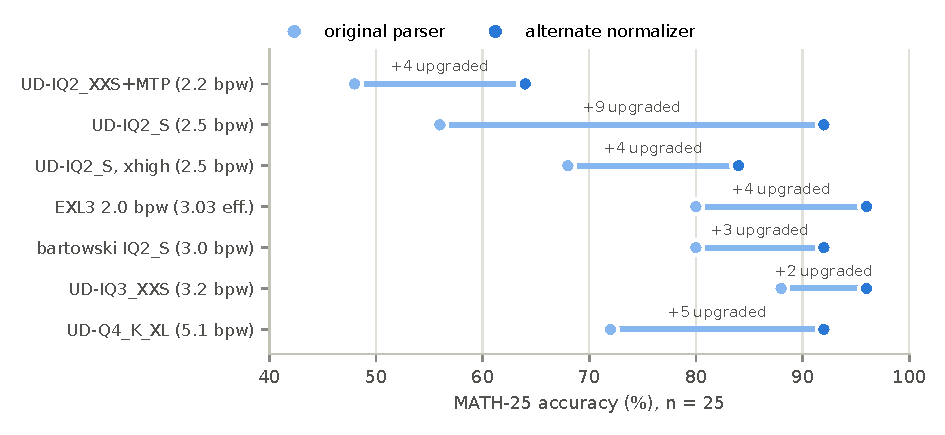
\includegraphics[width=\textwidth]{fig_artifact.pdf}
\caption{Original$\rightarrow$alternate score changes on MATH-25 ($n{=}25$).
The connector shows how many responses the post-hoc normalizer accepts that
the original parser rejected; both endpoints remain visible because the
rescore is not independent ground truth. The largest change is 9/25 at 2.49 effective bpw, versus
2/25 at 3.25 effective bpw.}
\label{fig:artifact}
\end{figure}

\paragraph{Accuracy across artifacts.}
Under the post-hoc normalizer, the estimates from 2.49 to 5.22 effective bpw
are 92--96\% and are not resolved from one another at this sample size. The
2.16-effective-bpw artifact scored 16/25, compared with 23/25 at 2.49 bpw on
the same items: seven successes favored the 2.49-bpw artifact and none favored
2.16 bpw (paired exact $p{=}0.016$, exploratory and uncorrected). No GGUF was
tested between 2.16 and 2.49 effective bpw, so the experiment identifies a
difference between these artifacts, not a universal threshold.

\paragraph{Parser sensitivity.}
For \q{UD-IQ2\_S}, the post-hoc normalizer accepted 9/25 responses rejected by
the original parser; for \q{UD-IQ3\_XXS}, it accepted 2/25. On the paired
items, seven changed only for IQ2\_S and none only for IQ3\_XXS (exact
$p{=}0.016$, exploratory and uncorrected). This establishes that parser
acceptance changed the apparent gap unevenly in these saved outputs. It does
not establish that every newly accepted response is semantically correct, or
that quantization generally harms answer formatting before reasoning.
Parser-compatible output remains a real deployment capability, so both scores
are retained.

\paragraph{Execution-scored code.} Generated code is
extracted from a fenced block and then executed, so it avoids symbolic-answer
normalization but still treats a missing/malformed code block as failure. We did
not post-hoc rescore those format failures; Table~\ref{tab:hard} reports the
end-to-end parser and test outcome as deployed.


\subsection{Hard-Suite Accuracy}
\label{sec:phase2b}

\begin{table}[t]
\centering
\small
\caption{Hard-suite summary (reasoning-effort medium). HumanEval+ is
execution-scored ($n{=}20$), Wilson 95\% CIs. Correct/min uses the
alternate MATH-25 score and each run's summed logged HTTP-response wall time;
post-response parsing and code execution are excluded.
The xhigh HumanEval+ entry is the truncation-free re-run
(\S\ref{sec:effort}).}
\label{tab:hard}
\setlength{\tabcolsep}{4pt}
\begin{tabular}{lllrr}
\toprule
Config (eff.\ bpw) & MATH-25 (alternate) & HumanEval+ & \multicolumn{2}{c}{correct/min} \\
 & & & math & HE+ \\
\midrule
\q{UD-IQ2\_XXS}+MTP (2.16) & 64\% [44.5, 79.8] & 70\% [48.1, 85.5] & 0.69 & 1.99 \\
\q{UD-IQ2\_S} (2.49) & 92\% [75.0, 97.8] & 90\% [69.9, 97.2] & 0.73 & 1.40 \\
\q{UD-IQ2\_S}, xhigh (2.49) & 84\% [65.3, 93.6] & 80\% [58.4, 91.9] & 0.37 & 0.73 \\
EXL3 2.0\,bpw (3.03) & \textbf{96\%} [80.5, 99.3] & 90\% [69.9, 97.2] & \textbf{0.83} & \textbf{2.27} \\
\q{IQ2\_S} bartowski (3.06) & 92\% [75.0, 97.8] & 90\% [69.9, 97.2] & 0.38 & 0.86 \\
\q{UD-IQ3\_XXS} (3.25) & \textbf{96\%} [80.5, 99.3] & 90\% [69.9, 97.2] & 0.33 & 0.73 \\
\q{UD-Q4\_K\_XL} (5.22) & 92\% [75.0, 97.8] & \textbf{95\%} [76.4, 99.1] & 0.19 & 0.43 \\
\bottomrule
\end{tabular}
\end{table}

Table~\ref{tab:hard} collects the hard suites. The 2.16-effective-bpw artifact
has the lowest point estimate on both: 16/25 alternate MATH and 14/20
HumanEval+, compared with 23/25 and 18/20 for the 2.49-bpw artifact. Because
every configuration saw the same items, paired tests are appropriate. The
MATH comparison has seven IQ2\_S-only successes and no IQ2\_XXS-only successes
(exact two-sided $p{=}0.016$); HumanEval+ has four and zero, respectively
($p{=}0.125$). Thus these data resolve the MATH loss but not the code-suite
difference. We do not pool the two suites into a single significance test.

Above 2.16 effective bpw, alternate MATH estimates are 92--96\% and HumanEval+
estimates are 90--95\%; no difference is resolved at these sample sizes. That
is evidence for a plateau within this experiment, not proof that the artifacts
or formats are equivalent. It also reinforces why nominal ``2-bit'' is too
coarse a label: the evaluated files bearing it span 2.16--3.06 effective bpw
and produced materially different hard-suite point estimates.


\subsection{Matched-Footprint Deployment Comparison}
\label{sec:exl3}

The EXL3 checkpoint is labeled 2.0\,bpw, but its 9.50\,GiB weight-file total is
\textbf{3.03 effective bpw}: the transformer weights target roughly 2\,bpw,
while the output head is 3-bit and other tensors are wider. It therefore is
not a footprint-matched comparison with the 6.77\,GiB, 2.16-effective-bpw
GGUF. Crediting their quality difference to trellis coding would confound
method with 40\% more effective bits.

The direct footprint control is bartowski \q{IQ2\_S}: 9.59\,GiB and 3.06
effective bpw. On identical hard-suite subsets, EXL3 scored 24/25 versus 23/25
on alternate MATH and both scored 18/20 on HumanEval+. These small samples do
not resolve a quality difference. They do expose a deployment difference: the
EXL3--ExLlamaV3 stack was fully GPU-resident, whereas the
bartowski-GGUF--llama.cpp stack offloaded six of 65 units. From the server logs
on these same workloads,
token-weighted generation throughput was 22.4 versus 13.7\,tok/s on MATH
($1.64\times$) and 30.7 versus 13.8\,tok/s on HumanEval+ ($2.22\times$).
The rate varies with output length and workload, so we use the MATH result as
the headline comparison: \textbf{at matched footprint, the fully resident
EXL3 deployment generated $1.6\times$ faster, and the available hard-suite
samples did not resolve a score difference.}

The other measured comparisons clarify what this result does and does not
identify:

\begin{itemize}
  \item At similar effective bpw, EXL3 (3.03) and \q{UD-IQ3\_XXS} (3.25)
  both scored 24/25 on alternate MATH and 18/20 on HumanEval+. We measured no
  quality-per-effective-bit advantage for either artifact at this point.
  \item Against \q{UD-IQ2\_XXS} (2.16), EXL3 has higher point scores but also
  a 2.73\,GiB larger file. This experiment cannot locate a trellis-specific
  quality boundary near 2.2 effective bpw.
\end{itemize}

This is the concrete sense in which the 12\,GB system exceeded a naive
capacity-based expectation: a 9.50\,GiB checkpoint remained resident and ran
at useful speed, while a nearly identical-size GGUF offloaded weights to RAM.
Because format and engine changed together, the experiment compares complete
deployments and cannot attribute the difference to trellis coding alone.

\begin{table}[t]
\centering
\small
\caption{Selected-deployment validation. MMLU used the same fixed 200-item,
57-subject-stratified subset; CIs are Wilson 95\%. Correct/min uses logged
HTTP-response wall time (post-response scoring excluded). Needle reports
probes completed correctly
before the client exhausted two 600-s HTTP attempts (one automatic retry),
not pure retrieval accuracy.}
\label{tab:validation}
\setlength{\tabcolsep}{5pt}
\begin{tabular}{lrrrl}
\toprule
Config & MMLU & Mean wall/item & Correct/min & Needle deadline success \\
\midrule
\q{UD-IQ2\_S} & 175/200, 87.5\% [82.2, 91.4] & 36.41\,s & 1.44 & 4/6 [30.0, 90.3] \\
EXL3 2.0\,bpw & 182/200, 91.0\% [86.2, 94.2] & 25.42\,s & 2.15 & 6/6 [61.0, 100] \\
\bottomrule
\end{tabular}
\end{table}

On paired MMLU items, both were correct on 171, only \q{UD-IQ2\_S} on four,
only EXL3 on 11, and neither on 14 (exact two-sided McNemar $p{=}0.119$).
The 3.5-point estimate therefore does not resolve a quality difference, while
EXL3 returned more correct items per minute. On the needle probes,
\q{UD-IQ2\_S} answered all four 8K/16K contexts but its two 32K items produced
no answer after two 600-s HTTP attempts each (one automatic retry after a
2-s delay, or about 1,202\,s total per item); EXL3 completed all six. The
4/6 versus 6/6 count measures completion under this client policy and includes
a large prompt-processing difference, so it must not be read as two wrong
retrieval answers.


\subsection{Reasoning-Effort Check}
\label{sec:effort}

Qwen3.8's chat template exposes a \q{reasoning\_effort} dial. For
\q{UD-IQ2\_S}, xhigh produced no observed benefit. On MATH-25 it scored
21/25 (84\%) under the alternate normalizer versus 23/25 (92\%) at medium,
with four rather than one 8K truncations. Mean wall time rose from 75.89 to
134.44\,s per item ($1.77\times$). On HumanEval+, an initial xhigh run was
truncation-confounded; the 8K-budget re-run removed truncations and scored
16/20 (80\%) versus 18/20 (90\%) at medium. Neither accuracy difference is
resolved at this sample size. The useful conclusion is narrower: xhigh was
slower and did not improve either point estimate in these runs, so medium is
the better measured setting for this deployment. This is not evidence that
additional reasoning effort is generally harmful.



\subsection{Correct Responses per Minute at Fixed VRAM}
\label{sec:metric}

\begin{figure}[t]
\centering
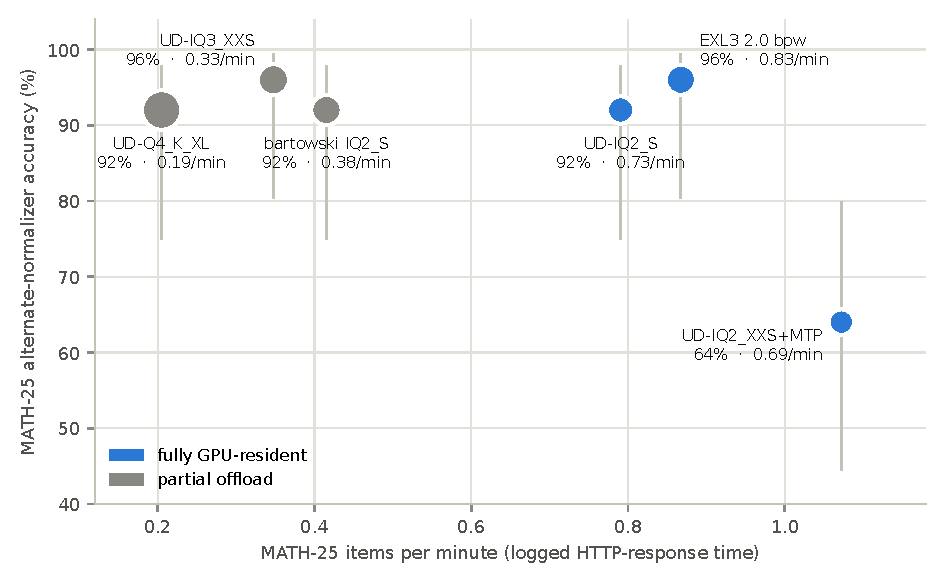
\includegraphics[width=\textwidth]{fig_frontier.pdf}
\caption{MATH-25 point estimates using logged HTTP-response time.
$x$: benchmark items completed per minute, whether correct or not; $y$:
alternate-normalizer accuracy with Wilson 95\% intervals; point area
$\propto$ file GiB. Their product is correct responses per minute. Colors
encode the measured residency state. The vertical intervals overlap widely;
the plot compares observed deployment rates and does not establish quality
dominance.}
\label{fig:frontier}
\end{figure}

For a fixed suite, correct responses per minute is the number scored correct
divided by summed per-item HTTP-response wall time. The timer includes prompt
processing, generation, retries, and request overhead, but stops before local
post-response parsing or code execution. It answers a deployment question---
how many successful model responses this machine returned per minute---without
pretending that a correct MATH item and a correct HumanEval+ item have the same
value. We therefore compare it only within a suite and always print the
underlying accuracy beside it.

The response-time view in Figure~\ref{fig:frontier} avoids the cross-engine
token/s problem: it prices prompt processing, generation length, retries,
request overhead, MTP, and offload as logged. It does not price local scoring.
On MATH-25, EXL3 has the highest observed
correct/min (0.83), followed by fully resident \q{UD-IQ2\_S} (0.73) and the
faster but less accurate \q{UD-IQ2\_XXS}+MTP (0.69). The partial-offload
artifacts range from 0.19 to 0.38. On HumanEval+, EXL3 has the highest
observed rate at 2.27, followed by the faster but lower-scoring
\q{UD-IQ2\_XXS}+MTP at 1.99 and \q{UD-IQ2\_S} at 1.40. These are efficiency
estimates on the observed subsets, not statistically distinct quality
rankings or a recommendation that ignores error cost.


\section{Discussion}
\label{sec:discussion}

\subsection{Deployment Recommendations}

For this machine, the measurements support distinct deployment choices.
Extrapolation to
other 12\,GB systems requires repeating the fit search because desktop VRAM,
engine buffers, and memory bandwidth change the boundary.

\begin{enumerate}
  \item \textbf{Default when the ExLlamaV3 stack is suitable: EXL3
  2.0\,bpw (3.03 effective).} It has the highest measured hard-suite
  correct/min and, among the two configurations selected for validation, the highest MMLU
  correct/min, with no resolved quality difference from the larger tested
  anchors. Its speed advantage is workload-dependent, and this run did not
  configure MTP or vision.
  \item \textbf{GGUF all-rounder: \q{UD-IQ2\_S}.} It remains fully resident,
  scored 92\%/90\% on the hard suites, and uses the llama.cpp/GGUF stack. The
  separate unsloth MTP draft did not fit in the measured desktop run state.
  \item \textbf{Maximum throughput when errors are cheaper:
  \q{UD-IQ2\_XXS}+MTP.} It delivered the fastest measured generation and
  6.01 correct GSM8K items/min, but its 64\% alternate MATH and 70\%
  HumanEval+ estimates were lower than the resident alternatives. It is not
  the recommendation for correctness-sensitive work.
\end{enumerate}


\subsection{Research Directions}

These measurements motivate a broader systems hypothesis: under a fixed VRAM
budget, useful single-stream throughput is often maximized by a deployment
that sits above the task-accuracy loss boundary but below the engine's
offload boundary. The present experiment establishes one instance, not a
general law. Testing the hypothesis requires repeating the same fit--speed--
accuracy map across models, engines, 8/12/16/24\,GB memory budgets, context
lengths, and power limits.

The highest-priority quality extension is a bf16, Q8, or hosted reference run
on hardware large enough to hold it. That would determine how much accuracy
all tested 12\,GB deployments lose relative to the original model; the current
Q4 anchor only supports comparisons within this experiment. Denser sampling
between 2.16 and 2.49 effective bpw, larger hard-task sets, and repeated
generations would test whether the observed GGUF drop is stable.

A method-level EXL3 claim would require tighter controls over tensor
precision, packaged components, kernels, and memory allocation, ideally with
one engine supporting both representations. The MATH audit can be strengthened
without rerunning inference: an independent, preregistered human or
computer-algebra review can rescore the archived predicted-answer fields. New inference
runs would be needed to estimate run-to-run variability or test whether
parser compatibility changes systematically with quantization.

\section{Limitations and Threats to Validity}
\label{sec:limitations}

\begin{itemize}
  \item \textbf{No unquantized quality reference.} We did not evaluate bf16,
  Q8, or the hosted model. Comparisons to \q{UD-Q4\_K\_XL} rank only the
  tested artifacts and do not establish parity with the original model.
  \item \textbf{Limited statistical power.} MATH-25 and HumanEval+ contain
  only 25 and 20 fixed items. Their Wilson intervals are wide; a non-significant
  comparison is not evidence of equality. MMLU is larger but tests a different
  capability mix. No correction was applied across the exploratory paired
  comparisons.
  \item \textbf{One stochastic sample.} Each item was generated once at
  temperature 1.0. The intervals quantify item sampling only, not variation
  across repeated generations.
  \item \textbf{Post-hoc alternate scoring.} The MATH normalizer was written
  after failures were inspected. Publishing its rules, retained per-item
  scoring records, original scores, and alternate scores makes the judgment
  auditable but does not make
  it independent or pre-registered.
  \item \textbf{Deployment, not method isolation.} The EXL3--GGUF comparison
  changes format, artifact, kernels, memory allocation, and engine together.
  It supports a choice between the tested deployments, not a causal claim
  about trellis coding.
  \item \textbf{Speed protocols.} The GGUF ladder uses controlled tg128 runs;
  no matching EXL3 microbenchmark was collected. Cross-engine ratios in
  \S\ref{sec:exl3} instead use engine-reported generation metrics on the same
  evaluation workloads. Correct/min uses logged HTTP-response wall time and is
  the more comparable deployment measure; it excludes local scoring time.
  \item \textbf{Scope and provenance.} Results come from one model, laptop,
  run state, and set of artifacts downloaded on one date. File sizes identify
  the local artifacts. Upstream revisions were recovered from the local cache
  after the campaign rather than emitted into the measurement logs at run
  time; the release records those revisions together with the exact file
  SHA-256 values. The 80\,W power limit is not an energy measurement, and no
  sustained thermal or per-watt conclusion is reported.
  \item \textbf{Long-context timeout contamination.} The two failed 32K
  \q{UD-IQ2\_S}+llama.cpp probes exhausted both 600-s HTTP attempts without
  returning an answer, so the needle comparison combines prompt-processing
  speed with retrieval behavior.
\end{itemize}



\section{Related Work}
\label{sec:related}

\textbf{Quantization methods.} This work evaluates existing post-training
quantization rather than introducing a method: GGUF k/i-quants in llama.cpp
\citep{gerganov2023llamacpp}, dynamic mixed-tensor GGUF recipes
\citep{unsloth2026dynamic}, and EXL3 \citep{turboderp2025exllamav3}, whose
trellis construction builds on QTIP \citep{tseng2024qtip}. GPTQ (published at
ICLR as OPTQ)
\citep{frantar2022gptq}, AWQ \citep{lin2023awq}, and ParetoQ
\citep{liu2025paretoq} provide broader calibration and low-bit scaling context.
Our effective-bpw accounting is a deployment-footprint measure, not a new
quantization metric.

\textbf{Post-freeze update (checked 2026-08-29).}
On 2026-08-28, after our 2026-08-25 artifact freeze, ISTA-DASLab released
Qwen3.8-27B checkpoints that use GSQ for low-bit scalar quantization and RCO
for per-tensor GGUF-type assignment under a file-size budget
\citep{dadgarnia2026gsq,helcig2026rco,istadaslab2026qwen38gsqrco}. They are
standard GGUF files, not a GSQ/RCO-specific runtime modification; we did not
evaluate their quality, residency, or correct/min on this system.

\textbf{Evaluation and answer parsing.} Prior work shows that aggregate task accuracy
can conceal important changes under quantization \citep{dutta2024accuracy},
and low-bit mathematical reasoning has been studied through process and error
taxonomies \citep{quantreasoning2025,extremelowbit2026}. Separately, structured
output research distinguishes semantic correctness from machine usability
\citep{correctnotusable2026}, while evaluation scaffolding can materially alter
measured outcomes \citep{scaffolding2026}. Task difficulty and instruction
following also interact with quantization \citep{quantinstruct2024}. Our
MATH audit is a small, concrete instance of these broader warnings: a
post-hoc alternate normalizer changed the apparent low-bit gap, so the
original-parser and post-hoc-normalized scores must remain visible. Community measurements that report strict or
machine-usable output rates provide a related operational view
\citep{strix2026}.

\textbf{Extreme-low-bit and cross-format comparisons.} Bielik-Q2-Sharp
compares six academic extreme-2-bit methods on an 11B Polish model and finds
that rankings depend on method and summary metric \citep{bielik2026q2sharp}.
Broader unified GGUF evaluation reports FP16, size, perplexity, throughput, and
standard downstream tasks on Llama-3.1-8B \citep{kurt2026whichquant}; a
contemporaneous Qwen3.8-27B study compares bf16 through 1-bit GGUFs on larger
datacenter GPUs \citep{migdal2026qwen38}. Those studies provide wider precision
or task coverage; the present question is the realized 12\,GB deployment
boundary.
EXL3's documentation reports its own quality curves
\citep{turboderp2025exllamav3}; an earlier matched-bpw community comparison
reported lower MMLU for lower-bpw EXL2 variants than for GGUF at matched
quantized-layer bpw on Llama~3 \citep{mattc1llama3}. Our data should not be
read as a method-level reversal of either result. At roughly 3 effective bpw we
resolve no hard-suite quality difference; the contribution is a matched-file-
footprint deployment comparison in which the EXL3 artifact remains resident
and the GGUF control does not.

\textbf{Local inference under resource constraints.} Bench360 evaluates
quality, latency, energy, and Pareto tradeoffs under a fixed 24\,GB budget
\citep{bench360}; other work studies accuracy--performance tradeoffs on server
GPUs \citep{kurtic2024bf16}, joint performance, energy, and quality under
online GPU serving \citep{qmeter2025}, and various combinations of latency,
quality, and energy on mobile, edge, or private-server systems
\citep{sustainableedge2025,palmbench2024,privateserver2025}. Silicon Showdown describes the consumer ``VRAM wall'' and
the throughput cost of CPU offload \citep{javat2026siliconshowdown}, while
pipelined sub-layer sharding targets that cost with a new client inference
system \citep{ukarande2026vram}.

Most directly, Moreira reports Qwen3.8-27B on a 12\,GB RTX~4070~Ti: a fully
resident IQ2 configuration generated at 43.643 tokens/s versus 5.977 for a
partially offloaded IQ4\_XS, while a 24-item custom suite favored IQ4\_XS
13--9 without resolving the paired difference \citep{moreira2026qwen38}.
Its desktop hardware, artifact, runtime, context, and speed protocol differ
from ours, so those absolute rates are prior evidence about the fit--offload
trade rather than a throughput baseline for this study.
Thus our study is not the first task-level fit-versus-offload measurement for
this model and memory class. It contributes an independent 80\,W laptop
characterization with standard task families, effective-footprint and
engine-residency accounting, a matched-footprint EXL3/GGUF deployment pair,
and an explicit parser audit. Correct/min is a descriptive within-suite
task-goodput rate, not a proposed universal or novel benchmark.

Our MTP measurements are an instance of speculative decoding
\citep{leviathan2022speculative,chen2023speculative}; they do not evaluate
speculative-decoding algorithms themselves.


\section{Artifact Availability and Reproducibility}
\label{sec:repro}

Every reported result traces to archived JSONL data alongside the harness:
\begin{itemize}
  \item fit searches, \q{llama-bench} results, timings, and VRAM peaks in
  \path{testsuite/results/phase1.jsonl};
  \item per-suite summaries in
  \path{testsuite/evals/results/summary.jsonl}; and
  \item per-item JSONL scoring records in each retained configuration's
  results directory, including predicted and expected answer fields and the
  final 200 characters of each saved response where applicable.
\end{itemize}
The alternate MATH-25 numbers come from the deterministic $\sim$50-line
\path{testsuite/evals/rescore_math25.py}; every rule is listed in
\S\ref{sec:artifact}. Figures are generated directly from these logs by
\path{paper/scripts/make_figures.py}. Engine server logs preserve the per-request
metrics used for the matched-workload comparison.

Software: llama.cpp master \q{b1-1729ed5}, CUDA 12.6.3 (user-local
toolchain), SM 8.9, flash-attn on; ExLlamaV3 1.4.3 under TabbyAPI
(\q{max\_seq\_len} 16384 for the main hard suites and 36864 for validation).
Artifacts: unsloth \q{Qwen3.8-27B-GGUF} UD tier,
bartowski \q{Qwen3.8-27B-GGUF} \q{IQ2\_S}, turboderp EXL3 \q{SC\_2.00bpw\_H3}
all downloaded 2026-08-25. File sizes in Table~\ref{tab:artifacts} identify
the local artifacts; the release manifest records every tested upstream
revision, filename, byte count, and SHA-256. Evaluation ran through each
engine's OpenAI-compatible endpoint; \q{reasoning\_effort} was passed per
request via \q{chat\_template\_kwargs}. Harness safety rules (VRAM fit guard
including the 1.2\,GiB \q{-ngld 0} draft-buffer correction, mmap-backed CPU
weights, one model process at a time) are documented in the harness and were
calibrated against the measured peaks in Table~\ref{tab:phase1}.

The public artifact should be used in two modes: an analysis-only path that
rebuilds tables and figures from archived logs without launching inference,
and a prospective replication path that downloads the pinned model artifacts
and reruns the GPU harness. The accompanying artifact includes a paper-specific README,
environment and hardware requirements, model revisions and checksums, concrete
setup and launch commands, expected outputs, and an immutable tag or archive
identifier. The version-of-record compendium is archived at
\href{https://doi.org/10.5281/zenodo.22166977}{doi:10.5281/zenodo.22166977};
the matching tagged source and results tree is
\url{https://github.com/matthematics1137/research-artifacts/tree/qwen38-27b-12gb-v1.0.0/papers/2026-qwen38-27b-12gb}.
The ML-facing result dataset is
\url{https://huggingface.co/datasets/mv1137/qwen38-27b-12gb-results}.
Full response transcripts were not retained: the per-item files contain scoring fields and
short answer excerpts. The Q4 easy-suite runs also lack per-item GSM8K and
HumanEval files and are supported only by their frozen aggregate summary rows.
We preserve these gaps rather than reconstructing records after the fact.


\section{Conclusion}

On the tested 12\,GB laptop, the best measured way to run Qwen3.8-27B was not
to load the largest artifact possible and accept CPU offload. Fully resident
GGUFs decoded at 24--25 tokens/s, while progressively offloaded GGUFs fell to
16.6--4.9 tokens/s. A 9.50\,GiB EXL3 checkpoint remained resident under
ExLlamaV3; compared with a 9.59\,GiB GGUF under llama.cpp, it generated
$1.6\times$ faster on MATH, had no hard-suite score difference resolved at the
available sample sizes, and produced the highest observed correct responses
per minute on MATH and HumanEval+.

The practical result is that this 12\,GB system ran a 27.4B model without the
repeated RAM weight reads that dominated the larger GGUF deployments. Finding
that operating point required the actual checkpoint footprint, engine memory
behavior, GPU residency, response time, and answer parser; the advertised bit
label alone was insufficient. This experiment does not establish parity with
bf16 or Q8, a universal optimum, or a trellis-specific advantage. Broader
claims require larger repeated evaluations, an unquantized or near-lossless
reference, and replication across models, engines, and memory budgets.

\medskip
\noindent\textbf{AI assistance.} Claude (Anthropic) and Codex (OpenAI) assisted
with evaluation-harness development, experiment execution, evidence auditing,
analysis and figure code, and manuscript drafting and revision. Matthew
Schwartz directed the work, reviewed and verified the retained outputs against
the archived evidence and cited sources, edited the manuscript, and takes full
responsibility for the methods, results, interpretation, citations, and
released artifacts.

\bibliographystyle{unsrtnat}
\bibliography{references}

% ===========================================================================

\end{document}
.
% When ON: near-black blue-warm page, light-gray body text (never pure white,
% to avoid halation), brighter section heads, soft cyan/amber links, salmon
% figures/dark/ (generated by scripts/make_figures.py --dark).
\newif\ifdarkmode
\ifdefined\DARKMODE
  \darkmodetrue
\else
  \darkmodefalse
\fi

\ifdarkmode
  % Visual definitions shared with explainer.tex (pure extraction, no
  % behavior change): colors, \pagecolor, default-color patch, \hypersetup,
  % bright section heads.
  \input{darkstyle}
  \graphicspath{{figures/dark/}}
\else
  \graphicspath{{figures/}}
\fi
% ---------------------------------------------------------------------------


% Quant names appear constantly; keep them readable.
\newcommand{\q}[1]{\texttt{#1}}
\newcommand{\singleauthorinfo}[1]{\\[0.25em]{\small #1}}

\title{\textbf{Deploying Qwen3.8-27B in 12\,GB of VRAM: Accuracy and
Throughput Across Quantized Inference Stacks}}

\hypersetup{
  pdftitle={Deploying Qwen3.8-27B in 12 GB of VRAM: Accuracy and Throughput Across Quantized Inference Stacks},
  pdfauthor={Matthew Schwartz},
  pdfsubject={Quantized large-language-model inference under a 12 GB GPU memory budget}
}

\author{Matthew Schwartz\singleauthorinfo{Independent researcher \enspace
\href{https://orcid.org/0009-0009-4171-7247}{ORCID 0009-0009-4171-7247}
\enspace \texttt{matthew.schwartz.research@gmail.com}}}

\date{August 29, 2026}

\begin{document}
\maketitle

\begin{abstract}
\noindent
Quantized-inference studies usually report quality under a fixed engine or
throughput under a fixed quantization, but a 12\,GB GPU couples these choices:
weights, cache, and engine buffers must fit together, and spilled weights are
read from slower system RAM. We characterize this deployment problem for
Qwen3.8-27B on an 80\,W RTX 4080 Laptop GPU by measuring fit, throughput, and
task performance for eight artifacts across GGUF/llama.cpp and
EXL3/ExLlamaV3. Fully resident GGUFs decoded at 24.4--25.5 tokens/s, whereas
partial offload reduced decode to 16.6--4.9 tokens/s. At approximately
9.5\,GiB file footprint, EXL3/ExLlamaV3 remained fully resident while
GGUF/llama.cpp offloaded six of 65 units; the hard-suite samples did not
resolve an accuracy difference, but EXL3 generated $1.6\times$ faster on MATH
and achieved the highest observed correct responses per minute on MATH and
HumanEval+. Across GGUF, the 2.16-effective-bpw artifact lost seven paired
MATH items relative to the 2.49-effective-bpw artifact, while configurations
from 2.49 to 5.22 effective bpw were not separated at these sample sizes; the
original MATH parser also disagreed with the post-hoc normalizer unevenly
across artifacts, so we report both scores separately. On this machine, joint
artifact--engine selection kept a 27.4B model in 12\,GB of VRAM and delivered
correct responses faster than partial offload, with no hard-task difference
resolved relative to the largest tested artifact; we did not test bf16 or Q8,
or isolate engine from format.
\end{abstract}



\section{Introduction}
\label{sec:intro}

Quantized-inference work usually reports either quality under a fixed engine or
throughput under a fixed quantization. A 12\,GB discrete GPU couples the two:
the file, cache, and engine buffers must fit together, and crossing that boundary
moves weight reads from high-bandwidth VRAM to much slower system RAM. The
practical question is therefore not simply ``which quant has the best quality?''
It is: \emph{which artifact--engine pair returns correct answers fastest inside
this fixed memory budget?}

We answer that question for Qwen3.8-27B, whose 27.36 billion non-MTP VLM
parameters would require roughly 54.7\,GB at bf16 before runtime overhead, on
one 12\,GB laptop GPU. In
the measured run state, the right low-bit artifact and engine kept the model
fully GPU-resident. Its scores on the small hard-task suites were not resolved
from those of the largest tested artifact, and it returned more correct answers
per minute than the larger deployments that placed weights in system RAM. This
is the paper's central result: the machine did more useful work with a smaller,
fully resident deployment than with the largest tested, partially offloaded
artifact, which kept only 33 of 65 offload units on the GPU. More useful work
here means more correctly scored responses per minute, not a resolved
raw-accuracy advantage.

We first found the maximum GPU-resident layer count and measured prompt and
decode throughput for a GGUF ladder. We then evaluated selected configurations
on easy and harder task subsets, inspected MATH scoring failures item by item,
added a GGUF control with nearly the same file footprint as EXL3, and compared
the two recommended deployments on MMLU and long-context probes. We report
nominal quantization, actual checkpoint size, GPU residency, task score, and
wall-clock response rate separately.

\paragraph{Contribution and scope.}
The primary contribution is an end-to-end deployment map for a 27.4B model
under a 12\,GB laptop-GPU memory budget. It connects checkpoint footprint and
engine-specific residency to controlled throughput, benchmark accuracy, and
correct responses per minute. Fully resident GGUFs decoded at 24--25 tokens/s,
whereas progressively offloaded GGUFs fell to 16.6--4.9 tokens/s. At matched
file footprint, EXL3/ExLlamaV3 remained resident and generated faster than
GGUF/llama.cpp without a resolved hard-suite score difference.

Two audits qualify that result. Nominal bit labels did not reliably predict
whole-checkpoint size, and the post-hoc MATH normalizer accepted some surface
forms that the original parser rejected. We therefore compare complete artifact--engine
deployments rather than attributing the cross-stack result to trellis coding,
and report the original-parser score beside a disclosed post-hoc-normalized
score. The latter is a rescore of saved outputs, not an independent semantic
ground truth.

The hard-suite subsets are small ($n{=}20$--$25$), every generation is a single
sample at temperature 1.0, and engine and format cannot be separated in the
cross-ecosystem comparison. Wilson 95\% intervals accompany every accuracy.
These data characterize the tested deployments; they do not establish model-
or hardware-class generalities (\S\ref{sec:limitations}).


\section{Experimental Setup}
\label{sec:setup}

\subsection{Hardware}
\label{sec:hw}

All measurements were taken on a single consumer laptop: NVIDIA GeForce RTX
4080 Laptop GPU (Ada Lovelace, SM~8.9), 12{,}282\,MiB VRAM, capped at
\textbf{80\,W}; Intel Core i9-14900HX CPU; 62\,GiB dual-channel DDR5; NVMe
storage; Linux 7.0.0, driver 580.167.08. The desktop session held
$\sim$900\,MiB of VRAM, leaving a measured working envelope of roughly
10.5--11\,GiB for weights, cache/state, and compute buffers. Power mode, memory
clock, and sustained device clocks were not separately logged; the throughput
results therefore describe this run state, not a normalized hardware limit.

Batch-one dense decode is usually memory-bandwidth-bound: each generated
token's forward pass uses the active weight set, which is too large to remain
in on-chip cache, so memory traffic scales approximately with active weight
bytes and $\text{tok/s} \approx
\text{effective bandwidth}/\text{bytes per token}$. The laptop's GDDR6 is
$\sim$432\,GB/s on paper; our fitted effective GPU-resident weight-path
bandwidth is 199\,GB/s (\S\ref{sec:offload}). The fitted CPU-resident
weight-path coefficient is 41\,GB/s---roughly $5\times$ lower. It absorbs
memory-transfer and decode effects and is not a raw DDR5 specification. This
two-bandwidth model is descriptive of the observed GGUF ladder;
quant-family-specific CPU kernels account for its largest residuals.


\subsection{Model}
\label{sec:model}

Qwen3.8-27B (released 2026-08-14) is an instruction-tuned vision--language
model with 26.896B main-language parameters and 0.461B vision parameters
(27.36B non-MTP parameters, rounded to 27.4B here). Its separate MTP head has
0.425B parameters. The model card reports a
\emph{hybrid} sequence mixer: only 16 of 64 layers are classical attention
with a growing KV cache (4~KV heads $\times$ 256 head dim), while the other 48
are DeltaNet-style linear-attention layers \citep{qwen38model}. Gated Delta
Networks and Mamba provide the architectural background
\citep{yang2024gateddeltanet,gu2023mamba}; the recurrent layers hold a
constant-size state ($\sim$150\,MB total here). Verified KV cost is
$2 \times 4 \times 256 \times 2\,\text{B} \times 16 = \mathbf{64\,KiB/token}$
at fp16 ($\sim$38\,KiB at q8\_0) --- $4\times$ lower than a counterfactual
64-layer model using the same four-KV-head attention block in every layer. At
the tested context lengths, KV-memory growth was therefore
relatively cheap and \emph{fitting was primarily a weights problem}. The
release ecosystem also provides a 1.28\,GiB multi-token-prediction (MTP) head;
the tested llama.cpp build used it as an in-model draft
\citep{qwen38model,gerganov2023llamacpp}, an instance of speculative decoding
\citep{leviathan2022speculative,chen2023speculative}. It also provides a
0.86\,GiB vision
projector (vision was not evaluated). These components are packaged
differently: the unsloth GGUF release stores both separately, the bartowski
GGUF embeds the MTP tensors, and the tested EXL3 checkpoint has no configured
draft or vision path. The 248K-token vocabulary makes the text embeddings a
large, hard-to-quantize fraction of every weight artifact --- one reason
nominal and effective bits-per-weight diverge (Table~\ref{tab:artifacts}).


\subsection{Engines}
\label{sec:engines}

Two inference stacks: \textbf{llama.cpp} \citep{gerganov2023llamacpp} built
from master at \q{b1-1729ed5} with a user-local CUDA 12.6.3 toolchain
(SM~8.9), serving GGUF artifacts with layer-wise CPU offload (\q{-ngl}); and
\textbf{ExLlamaV3 1.4.3} \citep{turboderp2025exllamav3} via TabbyAPI, serving
EXL3 trellis-quantized safetensors. For this tested dense checkpoint, the stack
used no supported dense-layer CPU weight-offload path, so the complete model
had to fit in VRAM. Unless noted:
context 8192, KV cache q8\_0, flash attention on, the model card's recommended
thinking-mode sampling (temperature 1.0, top-p 0.95, top-k 20)
\citep{qwen38model}, and the chat template's
\q{reasoning\_effort} set to \emph{medium}.


\subsection{Artifacts}
\label{sec:artifacts}

Table~\ref{tab:artifacts} lists the eight evaluated weight artifacts with their
measured checkpoint weight-file total and \emph{effective} bits per weight,
computed as $8B/26{,}895{,}998{,}464$ for total weight-file bytes $B$ and the
exact main-language parameter count. We report effective bpw beside every
nominal label throughout the paper; the two diverge by up to 52\% and the
difference determines which artifacts are valid footprint controls in
\S\ref{sec:exl3}.

\begin{table}[t]
\centering
\small
\caption{Eight evaluated weight artifacts. Effective bpw
$=8B/26{,}895{,}998{,}464$ for checkpoint weight-file total $B$, normalized
by the exact main-language parameter count; it can exceed the nominal label because embeddings
(248K vocabulary), norms, and (for EXL3) the 3-bit head quantize wider than the
label. Downloaded 2026-08-25 from \q{unsloth/Qwen3.8-27B-GGUF},
\q{bartowski/Qwen3.8-27B-GGUF}, and turboderp's EXL3 conversions
(\q{SC\_2.00bpw\_H3}). The optional unsloth MTP draft is listed separately and
is not included in its target file size.}
\label{tab:artifacts}
\setlength{\tabcolsep}{4pt}
\begin{tabular}{llrrl}
\toprule
Artifact & Format & File & Eff.\ bpw & Note \\
\midrule
\q{UD-IQ2\_XXS} & GGUF i-quant, unsloth UD & 6.77\,GiB & 2.16 & smallest under test \\
\q{UD-IQ2\_S} & GGUF i-quant, unsloth UD & 7.80\,GiB & 2.49 & largest full-GPU fit \\
\q{UD-Q2\_K\_XL} & GGUF k-quant, unsloth UD & 9.15\,GiB & 2.92 & \\
\q{IQ2\_S} (bartowski) & GGUF i-quant & 9.59\,GiB & 3.06$^{a}$ & MTP head baked in \\
\q{UD-IQ3\_XXS} & GGUF i-quant, unsloth UD & 10.18\,GiB & 3.25 & \\
\q{UD-IQ3\_S} & GGUF i-quant, unsloth UD & 11.21\,GiB & 3.58 & \\
\q{UD-Q4\_K\_XL} & GGUF k-quant, unsloth UD & 16.35\,GiB & 5.22 & largest quality anchor \\
EXL3 2.0\,bpw & EXL3 trellis (QTIP-style) & 9.50\,GiB & 3.03 & nominal 2.0; head at 3\,bpw \\
\midrule
Optional MTP draft & GGUF Q4\_0 & 1.28\,GiB & --- & separate for unsloth targets \\
\bottomrule
\multicolumn{5}{l}{\footnotesize $^{a}$Includes the baked-in MTP head, so main-model bpw is lower.}
\end{tabular}
\end{table}


\subsection{Evaluation Protocol and Metrics}
\label{sec:harness}

The fit-and-throughput campaign used a guarded harness (never launch unless estimated VRAM $\leq$
free$-$500\,MiB and available RAM covers CPU-resident bytes $+8$\,GiB; weights
always mmap-backed) that runs, per artifact: a fit search for the maximum
GPU-resident layer count at ctx 8192, \q{llama-bench} pp512/tg128 at that fit,
and timed \q{llama-server} generations (prose and code prompts, MTP off/on).
llama.cpp reports 65 offload units for this 64-block model because its count
includes the output layer. Each result is written and flushed to JSONL
immediately.

The accuracy campaign evaluated served models through the OpenAI-compatible endpoint on four
suites: \textbf{GSM8K} \citep{cobbe2021gsm8k} $\times 50$, strict answer
extraction; \textbf{HumanEval} \citep{chen2021humaneval} $\times 20$, generated
code executed against the official tests; \textbf{MATH-25}: 25 competition
problems at MATH levels 4--5 \citep{hendrycks2021math}, 8K-token generation
budget, truncations scored wrong; and \textbf{HumanEval+} $\times 20$
\citep{liu2023evalplus}, execution against EvalPlus's $\sim$80$\times$
augmented test sets. Every accuracy in this paper carries a Wilson 95\%
interval in brackets. The subsets were sampled deterministically with seed 42;
MATH-25 was stratified across all seven subjects, and HumanEval+ used the same
20 problems as HumanEval. A final validation compared the two selected
deployments on a 200-item, 57-subject-stratified MMLU subset
\citep{hendrycks2021mmlu} and six synthetic
needle contexts (8K/16K/32K, two insertion depths). For MATH, the
\emph{original-parser score} applies the answer extractor and acceptance rules
used during the run. The \emph{post-hoc-normalized score} applies a disclosed,
deterministic normalizer to the same saved responses; it does not regenerate
answers and is not an independent judgment of semantic correctness. At
$n{=}20$--$25$ the
intervals are wide. They reflect item sampling, not the additional variation
from single stochastic generations.



\section{Results}
\label{sec:phase1}

\subsection{GPU Residency and Throughput}

\begin{table}[t]
\centering
\footnotesize
\setlength{\tabcolsep}{3.5pt}
\caption{Controlled GGUF speed matrix (llama.cpp \q{b1-1729ed5}; ctx 8192,
KV q8\_0, flash-attn on; desktop session running). tg = \q{llama-bench} tg128;
server-measured decode agreed within $\pm 0.4$\,tok/s. EXL3 is excluded because
no matching \q{tg128} measurement was collected; its workload measurements are
reported separately in \S\ref{sec:exl3}.}
\label{tab:phase1}
\begin{tabular}{lrrrrrl}
\toprule
Config & File & GPU layers & tg tok/s & pp512 & VRAM peak & MTP effect on tg \\
\midrule
\q{UD-IQ2\_XXS} & 6.8\,GiB & \textbf{65/65} & \textbf{25.5} & 733 & 8.6--8.9\,GiB & $+21\%\rightarrow$ 30.9 (GPU draft); \\
 & & & & & & \quad 48--50 math; $-16\%$ CPU draft \\
\q{UD-IQ2\_S} & 7.8\,GiB & \textbf{65/65} & \textbf{24.4} & 708 & 9.7--10.0\,GiB & draft misses fit by $\sim$100\,MiB \\
\q{UD-Q2\_K\_XL} & 9.2\,GiB & 61/65 & 16.6 & 652 & 10.0--10.4\,GiB & crashed (draft buffers, see text) \\
\q{IQ2\_S} (bartowski) & 9.6\,GiB & 59/65 & 13.8 & 580 & 9.5--10.2\,GiB & not tested \\
\q{UD-IQ3\_XXS} & 10.2\,GiB & 54/65 & 11.3 & 608 & 10.4--10.8\,GiB & crashed (draft buffers) \\
\q{UD-IQ3\_S} & 11.2\,GiB & 49/65 & 8.2 & 559 & 10.5--10.7\,GiB & crashed (draft buffers) \\
\q{UD-Q4\_K\_XL} & 16.4\,GiB & 33/65 & 4.9 & 361 & 10.5\,GiB & wash ($+8\%$ prose, $-8\%$ code) \\
\emph{CPU floor} (\q{UD-IQ2\_S}) & 7.8\,GiB & 0/65 & 3.3 & 4.1 & --- & --- \\
\bottomrule
\end{tabular}
\end{table}

\begin{figure}[t]
\centering
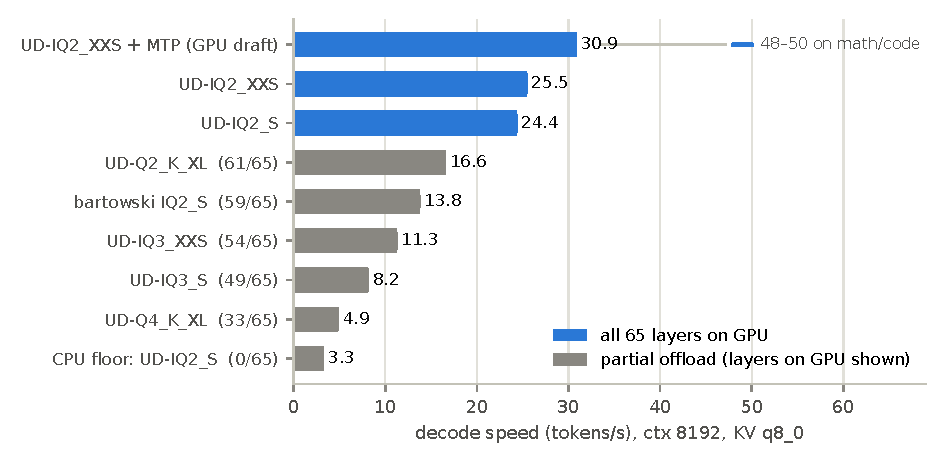
\includegraphics[width=\textwidth]{fig_ladder.pdf}
\caption{The measured speed ladder. Blue: all 65 layers GPU-resident; gray:
partial offload (GPU layer count in the label). The \q{UD-IQ2\_XXS}+MTP bar
shows prose decode; the whisker marks its measured 48--50\,tok/s on
math/code content (\S\ref{sec:mtp}). All base bars use the same
\q{llama-bench} tg128 protocol; the MTP annotations are separate server
measurements.}
\label{fig:ladder}
\end{figure}

Table~\ref{tab:phase1} and Figure~\ref{fig:ladder} give the matrix. The
full-residency boundary is the dominant feature; nominal labels and prompt
processing add two important qualifications.

\paragraph{For llama.cpp/GGUF, the full-GPU boundary lies between 7.8 and
9.2\,GiB in this run state.}
With the desktop session holding $\sim$900\,MiB, only the 6.8 and 7.8\,GiB
artifacts fit all 65 layers. Everything larger sheds layers to system RAM and
slows immediately. Within the GGUF ladder, footprint and consequent residency
are the first-order predictors of speed. This boundary is engine-specific:
ExLlamaV3 later fits a 9.50\,GiB EXL3 checkpoint (\S\ref{sec:exl3}).

\paragraph{The nominal quant label does not determine footprint or speed.}
Unsloth's \q{UD-IQ2\_S} (7.8\,GiB, 2.49 effective bpw) runs 24.4\,tok/s;
bartowski's \q{IQ2\_S} (9.6\,GiB, 3.06 effective bpw) runs 13.8\,tok/s. The
files share a nominal label but not a size, tensor allocation, or packaging:
the bartowski file also embeds MTP tensors. The observed speed difference is
consistent with full versus partial residency; it does not isolate a
quant-maker or allocation effect.

\paragraph{At 512 prompt tokens, GPU-heavy configurations ingest much faster
than they decode.} The controlled pp512 rates were 360--733\,tok/s, while the
CPU-only i-quant floor fell to 4.1\,tok/s. These short-context microbenchmarks
must not be extrapolated to 32K prompts; the deadline behavior in
\S\ref{sec:exl3} shows why.


\subsection{Offload Decay Follows a Two-Bandwidth Model}
\label{sec:offload}

\begin{figure}[t]
\centering
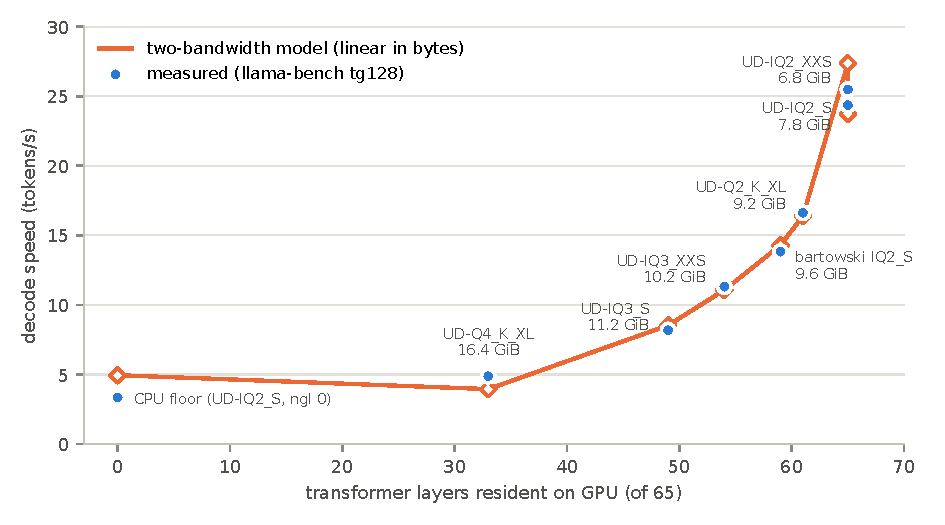
\includegraphics[width=\textwidth]{fig_offload.pdf}
\caption{Decode speed vs.\ GPU-resident layer count (blue, measured), with the
two-bandwidth model's per-config predictions (orange). The model, fitted for
relative error over all eight points, is
$1/\text{tok/s} = b_{\text{GPU}}/199\,\text{GB/s} +
b_{\text{CPU}}/41\,\text{GB/s}$ where $b$ are resident byte counts
(file bytes split proportionally to layers). The six non-extreme measured
states land within $\pm 8\%$; the two extremes' deviations are consistent with a
quant-family-dependent CPU term (i-quants dequantize expensively on CPU, so the ngl-0
floor runs $32\%$ below the pure-bandwidth prediction, while k-quant
\q{UD-Q4\_K\_XL} runs $24\%$ above it).}
\label{fig:offload}
\end{figure}

Figure~\ref{fig:offload} tests the bandwidth model of \S\ref{sec:hw} against
the matrix. Per-token time is linear in the two resident byte counts, with
fitted effective path bandwidths of \textbf{199\,GB/s} (GPU-resident bytes)
and \textbf{41\,GB/s} (CPU-resident bytes) --- a $4.9\times$ ratio, and the
reason each shed layer costs so much.
The fit's residual structure is itself informative: deviations concentrate
where CPU dequantization cost differs by quant family, i.e., the ``linear in
bytes'' rule needs a per-family CPU coefficient before it can be used
predictively across formats. For ranking configs on one family it is already
accurate to a few percent.


\subsection{MTP Benefit Depends on Workload and Placement}
\label{sec:mtp}

On the controlled prose prompt, the MTP draft head increased decode throughput by
21\% (25.5 $\rightarrow$ 30.9\,tok/s) at temperature 1.0 with the draft fully
on GPU, at a 41\% acceptance rate. During the MATH run, the same deployed
configuration produced 45--50 output tokens/s. That higher workload rate is
consistent with greater acceptance on structured text, but no draft-off run was
collected on the identical MATH prompts, so it is not a controlled 90\% MTP
effect. Likewise, the 9.6\,s mean GSM8K item time for
\q{UD-IQ2\_XXS}+MTP versus 17.7\,s for \q{UD-IQ2\_S} is a deployment
comparison, not an isolated MTP comparison: both the artifact and draft setting
change.

Two operational caveats. First, with the draft on CPU, MTP was a \emph{loss}
($-16\%$) or a wash in the controlled prose runs; these results should not be carried
over to other sampling regimes. Second, the draft's
VRAM cost is treacherous: $\sim$2.8\,GiB GPU-side when GPU-hosted, and still
$\sim$\textbf{1.2\,GiB} when nominally CPU-hosted (\q{-ngld 0}), because its
context and compute buffers allocate on the GPU regardless. This silently
crashed every tightly fitted mid-size config in our first sweep (the
``crashed'' rows of Table~\ref{tab:phase1}) until the harness guard learned to
account for it.

The result is therefore configuration-specific: MTP can help substantially
when the draft fits on GPU, but it is neither free in VRAM nor described by one
workload-independent speedup.



\subsection{Easy-Suite Accuracy Screen}
\label{sec:phase2}
\label{sec:phase2a}

\begin{table}[t]
\centering
\small
\caption{GSM8K ($n{=}50$) and HumanEval (executed, $n{=}20$) at
reasoning-effort medium, with Wilson 95\% CIs. Correct/min $=$ number of
successful items divided by summed logged HTTP-response wall time (local
post-response scoring excluded); compare only within a suite.}
\label{tab:phase2a}
\begin{tabular}{lrllrr}
\toprule
Config & tok/s & GSM8K & HumanEval & \multicolumn{2}{c}{correct/min} \\
 & & & & GSM8K & HE \\
\midrule
\q{UD-IQ2\_XXS}+MTP & 30.9 ($\approx$49 math) & 96\% [86.5, 98.9] & 80\% [58.4, 91.9] & \textbf{6.01} & 1.66 \\
\q{UD-IQ2\_S} & 24.4 & 94\% [83.8, 97.9] & \textbf{100\%} [83.9, 100] & 3.18 & \textbf{1.67} \\
\q{UD-Q2\_K\_XL} & 16.6 & 94\% [83.8, 97.9] & 100\% [83.9, 100] & 2.26 & 1.53 \\
\q{IQ2\_S} (bartowski) & 13.8 & 98\% [89.5, 99.6] & 95\% [76.4, 99.1] & 2.21 & 1.05 \\
\q{UD-IQ3\_XXS} & 11.3 & 96\% [86.5, 98.9] & 100\% [83.9, 100] & 1.65 & 0.92 \\
\q{UD-IQ3\_S} & 8.2 & 98\% [89.5, 99.6] & 100\% [83.9, 100] & 1.23 & 0.70 \\
\q{UD-Q4\_K\_XL} & 4.9 & 98\% [89.5, 99.6] & 100\% [83.9, 100] & 0.66 & 0.42 \\
\bottomrule
\end{tabular}
\end{table}

Table~\ref{tab:phase2a} has little resolution among the larger artifacts:
GSM8K estimates span 94--98\%, and HumanEval estimates span 95--100\% above
2.16 effective bpw. \q{UD-IQ2\_XXS} has the lowest HumanEval estimate (80\%),
but all intervals are wide. The practical difference is time. Across these two
suites, \q{UD-Q4\_K\_XL} used $4.6\times$ the pooled wall-clock of
\q{UD-IQ2\_S} ($7318\,\text{s}/1606\,\text{s}$) and recorded two additional
successes out of 70; no accuracy difference was resolved. Because these older
suites cluster near the top of their scales, the next experiments use the fixed MATH-25
subset and HumanEval+ to seek greater separation.


\subsection{MATH Answer-Parser Sensitivity}
\label{sec:artifact}

The original MATH parser scored \q{UD-IQ2\_S} at 14/25 and
\q{UD-IQ3\_XXS} at 22/25. Inspection of the saved responses found rejected
strings that differed from the reference in answer tags, math delimiters,
Unicode symbols, degree notation, brace shorthand, or an equation such as
\q{x=5} where the key contained \q{5}.

After inspecting those failures, we wrote a deterministic alternate
normalizer and applied it to every saved prediction. It accepts the declared
equivalences, leaves truncations wrong, and leaves mechanically unresolved
cases wrong. Because the rules were chosen post hoc, this score is not an
independent measure of mathematical correctness and does not replace the
original deployment parser. Table~\ref{tab:math25} and
Figure~\ref{fig:artifact} report both scores, with the rules and retained
per-item scoring records available for audit. No inference was rerun for this
analysis.

\begin{table}[t]
\centering
\small
\caption{MATH-25 ($n{=}25$, competition level 4--5): original parser score
vs.\ alternate-normalizer score, with the number of upgraded items
(value-equivalent under the alternate rules) and truncations (8K generation
budget exhausted; wrong under both scorers). Wilson 95\% CIs use the alternate
score. Reasoning-effort medium except where noted. Two \q{UD-Q4\_K\_XL} rows
lost their ground-truth field to a harness bug; the rescorer recovers them from
the dataset.}
\label{tab:math25}
\setlength{\tabcolsep}{5pt}
\begin{tabular}{lrrlcc}
\toprule
Config (eff.\ bpw) & Original & Alternate & CI (alternate) & Upgraded & Trunc. \\
\midrule
\q{UD-IQ2\_XXS}+MTP (2.16) & 12/25 & 16/25 (64\%) & [44.5, 79.8] & 4 & 3 \\
\q{UD-IQ2\_S} (2.49) & 14/25 & \textbf{23/25 (92\%)} & [75.0, 97.8] & \textbf{9} & 1 \\
\q{UD-IQ2\_S}, xhigh (2.49) & 17/25 & 21/25 (84\%) & [65.3, 93.6] & 4 & 4 \\
EXL3 2.0\,bpw (3.03) & 20/25 & \textbf{24/25 (96\%)} & [80.5, 99.3] & 4 & 1 \\
\q{IQ2\_S} bartowski (3.06) & 20/25 & 23/25 (92\%) & [75.0, 97.8] & 3 & 1 \\
\q{UD-IQ3\_XXS} (3.25) & 22/25 & \textbf{24/25 (96\%)} & [80.5, 99.3] & 2 & 0 \\
\q{UD-Q4\_K\_XL} (5.22) & 18/25 & 23/25 (92\%) & [75.0, 97.8] & 5 & 0 \\
\bottomrule
\end{tabular}
\end{table}

\begin{figure}[t]
\centering
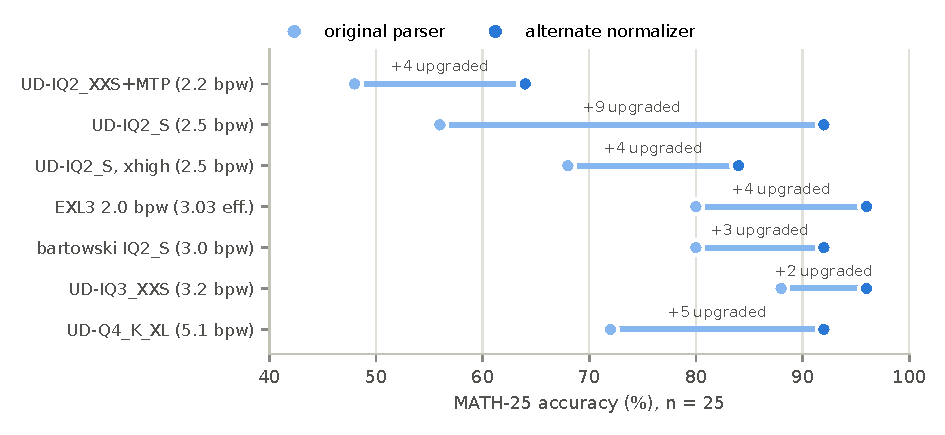
\includegraphics[width=\textwidth]{fig_artifact.pdf}
\caption{Original$\rightarrow$alternate score changes on MATH-25 ($n{=}25$).
The connector shows how many responses the post-hoc normalizer accepts that
the original parser rejected; both endpoints remain visible because the
rescore is not independent ground truth. The largest change is 9/25 at 2.49 effective bpw, versus
2/25 at 3.25 effective bpw.}
\label{fig:artifact}
\end{figure}

\paragraph{Accuracy across artifacts.}
Under the post-hoc normalizer, the estimates from 2.49 to 5.22 effective bpw
are 92--96\% and are not resolved from one another at this sample size. The
2.16-effective-bpw artifact scored 16/25, compared with 23/25 at 2.49 bpw on
the same items: seven successes favored the 2.49-bpw artifact and none favored
2.16 bpw (paired exact $p{=}0.016$, exploratory and uncorrected). No GGUF was
tested between 2.16 and 2.49 effective bpw, so the experiment identifies a
difference between these artifacts, not a universal threshold.

\paragraph{Parser sensitivity.}
For \q{UD-IQ2\_S}, the post-hoc normalizer accepted 9/25 responses rejected by
the original parser; for \q{UD-IQ3\_XXS}, it accepted 2/25. On the paired
items, seven changed only for IQ2\_S and none only for IQ3\_XXS (exact
$p{=}0.016$, exploratory and uncorrected). This establishes that parser
acceptance changed the apparent gap unevenly in these saved outputs. It does
not establish that every newly accepted response is semantically correct, or
that quantization generally harms answer formatting before reasoning.
Parser-compatible output remains a real deployment capability, so both scores
are retained.

\paragraph{Execution-scored code.} Generated code is
extracted from a fenced block and then executed, so it avoids symbolic-answer
normalization but still treats a missing/malformed code block as failure. We did
not post-hoc rescore those format failures; Table~\ref{tab:hard} reports the
end-to-end parser and test outcome as deployed.


\subsection{Hard-Suite Accuracy}
\label{sec:phase2b}

\begin{table}[t]
\centering
\small
\caption{Hard-suite summary (reasoning-effort medium). HumanEval+ is
execution-scored ($n{=}20$), Wilson 95\% CIs. Correct/min uses the
alternate MATH-25 score and each run's summed logged HTTP-response wall time;
post-response parsing and code execution are excluded.
The xhigh HumanEval+ entry is the truncation-free re-run
(\S\ref{sec:effort}).}
\label{tab:hard}
\setlength{\tabcolsep}{4pt}
\begin{tabular}{lllrr}
\toprule
Config (eff.\ bpw) & MATH-25 (alternate) & HumanEval+ & \multicolumn{2}{c}{correct/min} \\
 & & & math & HE+ \\
\midrule
\q{UD-IQ2\_XXS}+MTP (2.16) & 64\% [44.5, 79.8] & 70\% [48.1, 85.5] & 0.69 & 1.99 \\
\q{UD-IQ2\_S} (2.49) & 92\% [75.0, 97.8] & 90\% [69.9, 97.2] & 0.73 & 1.40 \\
\q{UD-IQ2\_S}, xhigh (2.49) & 84\% [65.3, 93.6] & 80\% [58.4, 91.9] & 0.37 & 0.73 \\
EXL3 2.0\,bpw (3.03) & \textbf{96\%} [80.5, 99.3] & 90\% [69.9, 97.2] & \textbf{0.83} & \textbf{2.27} \\
\q{IQ2\_S} bartowski (3.06) & 92\% [75.0, 97.8] & 90\% [69.9, 97.2] & 0.38 & 0.86 \\
\q{UD-IQ3\_XXS} (3.25) & \textbf{96\%} [80.5, 99.3] & 90\% [69.9, 97.2] & 0.33 & 0.73 \\
\q{UD-Q4\_K\_XL} (5.22) & 92\% [75.0, 97.8] & \textbf{95\%} [76.4, 99.1] & 0.19 & 0.43 \\
\bottomrule
\end{tabular}
\end{table}

Table~\ref{tab:hard} collects the hard suites. The 2.16-effective-bpw artifact
has the lowest point estimate on both: 16/25 alternate MATH and 14/20
HumanEval+, compared with 23/25 and 18/20 for the 2.49-bpw artifact. Because
every configuration saw the same items, paired tests are appropriate. The
MATH comparison has seven IQ2\_S-only successes and no IQ2\_XXS-only successes
(exact two-sided $p{=}0.016$); HumanEval+ has four and zero, respectively
($p{=}0.125$). Thus these data resolve the MATH loss but not the code-suite
difference. We do not pool the two suites into a single significance test.

Above 2.16 effective bpw, alternate MATH estimates are 92--96\% and HumanEval+
estimates are 90--95\%; no difference is resolved at these sample sizes. That
is evidence for a plateau within this experiment, not proof that the artifacts
or formats are equivalent. It also reinforces why nominal ``2-bit'' is too
coarse a label: the evaluated files bearing it span 2.16--3.06 effective bpw
and produced materially different hard-suite point estimates.


\subsection{Matched-Footprint Deployment Comparison}
\label{sec:exl3}

The EXL3 checkpoint is labeled 2.0\,bpw, but its 9.50\,GiB weight-file total is
\textbf{3.03 effective bpw}: the transformer weights target roughly 2\,bpw,
while the output head is 3-bit and other tensors are wider. It therefore is
not a footprint-matched comparison with the 6.77\,GiB, 2.16-effective-bpw
GGUF. Crediting their quality difference to trellis coding would confound
method with 40\% more effective bits.

The direct footprint control is bartowski \q{IQ2\_S}: 9.59\,GiB and 3.06
effective bpw. On identical hard-suite subsets, EXL3 scored 24/25 versus 23/25
on alternate MATH and both scored 18/20 on HumanEval+. These small samples do
not resolve a quality difference. They do expose a deployment difference: the
EXL3--ExLlamaV3 stack was fully GPU-resident, whereas the
bartowski-GGUF--llama.cpp stack offloaded six of 65 units. From the server logs
on these same workloads,
token-weighted generation throughput was 22.4 versus 13.7\,tok/s on MATH
($1.64\times$) and 30.7 versus 13.8\,tok/s on HumanEval+ ($2.22\times$).
The rate varies with output length and workload, so we use the MATH result as
the headline comparison: \textbf{at matched footprint, the fully resident
EXL3 deployment generated $1.6\times$ faster, and the available hard-suite
samples did not resolve a score difference.}

The other measured comparisons clarify what this result does and does not
identify:

\begin{itemize}
  \item At similar effective bpw, EXL3 (3.03) and \q{UD-IQ3\_XXS} (3.25)
  both scored 24/25 on alternate MATH and 18/20 on HumanEval+. We measured no
  quality-per-effective-bit advantage for either artifact at this point.
  \item Against \q{UD-IQ2\_XXS} (2.16), EXL3 has higher point scores but also
  a 2.73\,GiB larger file. This experiment cannot locate a trellis-specific
  quality boundary near 2.2 effective bpw.
\end{itemize}

This is the concrete sense in which the 12\,GB system exceeded a naive
capacity-based expectation: a 9.50\,GiB checkpoint remained resident and ran
at useful speed, while a nearly identical-size GGUF offloaded weights to RAM.
Because format and engine changed together, the experiment compares complete
deployments and cannot attribute the difference to trellis coding alone.

\begin{table}[t]
\centering
\small
\caption{Selected-deployment validation. MMLU used the same fixed 200-item,
57-subject-stratified subset; CIs are Wilson 95\%. Correct/min uses logged
HTTP-response wall time (post-response scoring excluded). Needle reports
probes completed correctly
before the client exhausted two 600-s HTTP attempts (one automatic retry),
not pure retrieval accuracy.}
\label{tab:validation}
\setlength{\tabcolsep}{5pt}
\begin{tabular}{lrrrl}
\toprule
Config & MMLU & Mean wall/item & Correct/min & Needle deadline success \\
\midrule
\q{UD-IQ2\_S} & 175/200, 87.5\% [82.2, 91.4] & 36.41\,s & 1.44 & 4/6 [30.0, 90.3] \\
EXL3 2.0\,bpw & 182/200, 91.0\% [86.2, 94.2] & 25.42\,s & 2.15 & 6/6 [61.0, 100] \\
\bottomrule
\end{tabular}
\end{table}

On paired MMLU items, both were correct on 171, only \q{UD-IQ2\_S} on four,
only EXL3 on 11, and neither on 14 (exact two-sided McNemar $p{=}0.119$).
The 3.5-point estimate therefore does not resolve a quality difference, while
EXL3 returned more correct items per minute. On the needle probes,
\q{UD-IQ2\_S} answered all four 8K/16K contexts but its two 32K items produced
no answer after two 600-s HTTP attempts each (one automatic retry after a
2-s delay, or about 1,202\,s total per item); EXL3 completed all six. The
4/6 versus 6/6 count measures completion under this client policy and includes
a large prompt-processing difference, so it must not be read as two wrong
retrieval answers.


\subsection{Reasoning-Effort Check}
\label{sec:effort}

Qwen3.8's chat template exposes a \q{reasoning\_effort} dial. For
\q{UD-IQ2\_S}, xhigh produced no observed benefit. On MATH-25 it scored
21/25 (84\%) under the alternate normalizer versus 23/25 (92\%) at medium,
with four rather than one 8K truncations. Mean wall time rose from 75.89 to
134.44\,s per item ($1.77\times$). On HumanEval+, an initial xhigh run was
truncation-confounded; the 8K-budget re-run removed truncations and scored
16/20 (80\%) versus 18/20 (90\%) at medium. Neither accuracy difference is
resolved at this sample size. The useful conclusion is narrower: xhigh was
slower and did not improve either point estimate in these runs, so medium is
the better measured setting for this deployment. This is not evidence that
additional reasoning effort is generally harmful.



\subsection{Correct Responses per Minute at Fixed VRAM}
\label{sec:metric}

\begin{figure}[t]
\centering
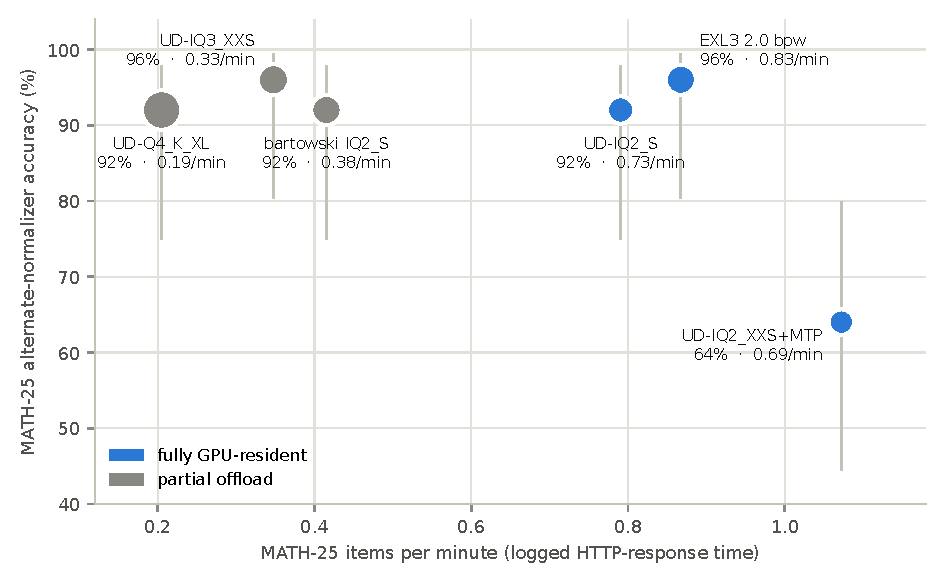
\includegraphics[width=\textwidth]{fig_frontier.pdf}
\caption{MATH-25 point estimates using logged HTTP-response time.
$x$: benchmark items completed per minute, whether correct or not; $y$:
alternate-normalizer accuracy with Wilson 95\% intervals; point area
$\propto$ file GiB. Their product is correct responses per minute. Colors
encode the measured residency state. The vertical intervals overlap widely;
the plot compares observed deployment rates and does not establish quality
dominance.}
\label{fig:frontier}
\end{figure}

For a fixed suite, correct responses per minute is the number scored correct
divided by summed per-item HTTP-response wall time. The timer includes prompt
processing, generation, retries, and request overhead, but stops before local
post-response parsing or code execution. It answers a deployment question---
how many successful model responses this machine returned per minute---without
pretending that a correct MATH item and a correct HumanEval+ item have the same
value. We therefore compare it only within a suite and always print the
underlying accuracy beside it.

The response-time view in Figure~\ref{fig:frontier} avoids the cross-engine
token/s problem: it prices prompt processing, generation length, retries,
request overhead, MTP, and offload as logged. It does not price local scoring.
On MATH-25, EXL3 has the highest observed
correct/min (0.83), followed by fully resident \q{UD-IQ2\_S} (0.73) and the
faster but less accurate \q{UD-IQ2\_XXS}+MTP (0.69). The partial-offload
artifacts range from 0.19 to 0.38. On HumanEval+, EXL3 has the highest
observed rate at 2.27, followed by the faster but lower-scoring
\q{UD-IQ2\_XXS}+MTP at 1.99 and \q{UD-IQ2\_S} at 1.40. These are efficiency
estimates on the observed subsets, not statistically distinct quality
rankings or a recommendation that ignores error cost.


\section{Discussion}
\label{sec:discussion}

\subsection{Deployment Recommendations}

For this machine, the measurements support distinct deployment choices.
Extrapolation to
other 12\,GB systems requires repeating the fit search because desktop VRAM,
engine buffers, and memory bandwidth change the boundary.

\begin{enumerate}
  \item \textbf{Default when the ExLlamaV3 stack is suitable: EXL3
  2.0\,bpw (3.03 effective).} It has the highest measured hard-suite
  correct/min and, among the two configurations selected for validation, the highest MMLU
  correct/min, with no resolved quality difference from the larger tested
  anchors. Its speed advantage is workload-dependent, and this run did not
  configure MTP or vision.
  \item \textbf{GGUF all-rounder: \q{UD-IQ2\_S}.} It remains fully resident,
  scored 92\%/90\% on the hard suites, and uses the llama.cpp/GGUF stack. The
  separate unsloth MTP draft did not fit in the measured desktop run state.
  \item \textbf{Maximum throughput when errors are cheaper:
  \q{UD-IQ2\_XXS}+MTP.} It delivered the fastest measured generation and
  6.01 correct GSM8K items/min, but its 64\% alternate MATH and 70\%
  HumanEval+ estimates were lower than the resident alternatives. It is not
  the recommendation for correctness-sensitive work.
\end{enumerate}


\subsection{Research Directions}

These measurements motivate a broader systems hypothesis: under a fixed VRAM
budget, useful single-stream throughput is often maximized by a deployment
that sits above the task-accuracy loss boundary but below the engine's
offload boundary. The present experiment establishes one instance, not a
general law. Testing the hypothesis requires repeating the same fit--speed--
accuracy map across models, engines, 8/12/16/24\,GB memory budgets, context
lengths, and power limits.

The highest-priority quality extension is a bf16, Q8, or hosted reference run
on hardware large enough to hold it. That would determine how much accuracy
all tested 12\,GB deployments lose relative to the original model; the current
Q4 anchor only supports comparisons within this experiment. Denser sampling
between 2.16 and 2.49 effective bpw, larger hard-task sets, and repeated
generations would test whether the observed GGUF drop is stable.

A method-level EXL3 claim would require tighter controls over tensor
precision, packaged components, kernels, and memory allocation, ideally with
one engine supporting both representations. The MATH audit can be strengthened
without rerunning inference: an independent, preregistered human or
computer-algebra review can rescore the archived predicted-answer fields. New inference
runs would be needed to estimate run-to-run variability or test whether
parser compatibility changes systematically with quantization.

\section{Limitations and Threats to Validity}
\label{sec:limitations}

\begin{itemize}
  \item \textbf{No unquantized quality reference.} We did not evaluate bf16,
  Q8, or the hosted model. Comparisons to \q{UD-Q4\_K\_XL} rank only the
  tested artifacts and do not establish parity with the original model.
  \item \textbf{Limited statistical power.} MATH-25 and HumanEval+ contain
  only 25 and 20 fixed items. Their Wilson intervals are wide; a non-significant
  comparison is not evidence of equality. MMLU is larger but tests a different
  capability mix. No correction was applied across the exploratory paired
  comparisons.
  \item \textbf{One stochastic sample.} Each item was generated once at
  temperature 1.0. The intervals quantify item sampling only, not variation
  across repeated generations.
  \item \textbf{Post-hoc alternate scoring.} The MATH normalizer was written
  after failures were inspected. Publishing its rules, retained per-item
  scoring records, original scores, and alternate scores makes the judgment
  auditable but does not make
  it independent or pre-registered.
  \item \textbf{Deployment, not method isolation.} The EXL3--GGUF comparison
  changes format, artifact, kernels, memory allocation, and engine together.
  It supports a choice between the tested deployments, not a causal claim
  about trellis coding.
  \item \textbf{Speed protocols.} The GGUF ladder uses controlled tg128 runs;
  no matching EXL3 microbenchmark was collected. Cross-engine ratios in
  \S\ref{sec:exl3} instead use engine-reported generation metrics on the same
  evaluation workloads. Correct/min uses logged HTTP-response wall time and is
  the more comparable deployment measure; it excludes local scoring time.
  \item \textbf{Scope and provenance.} Results come from one model, laptop,
  run state, and set of artifacts downloaded on one date. File sizes identify
  the local artifacts. Upstream revisions were recovered from the local cache
  after the campaign rather than emitted into the measurement logs at run
  time; the release records those revisions together with the exact file
  SHA-256 values. The 80\,W power limit is not an energy measurement, and no
  sustained thermal or per-watt conclusion is reported.
  \item \textbf{Long-context timeout contamination.} The two failed 32K
  \q{UD-IQ2\_S}+llama.cpp probes exhausted both 600-s HTTP attempts without
  returning an answer, so the needle comparison combines prompt-processing
  speed with retrieval behavior.
\end{itemize}



\section{Related Work}
\label{sec:related}

\textbf{Quantization methods.} This work evaluates existing post-training
quantization rather than introducing a method: GGUF k/i-quants in llama.cpp
\citep{gerganov2023llamacpp}, dynamic mixed-tensor GGUF recipes
\citep{unsloth2026dynamic}, and EXL3 \citep{turboderp2025exllamav3}, whose
trellis construction builds on QTIP \citep{tseng2024qtip}. GPTQ (published at
ICLR as OPTQ)
\citep{frantar2022gptq}, AWQ \citep{lin2023awq}, and ParetoQ
\citep{liu2025paretoq} provide broader calibration and low-bit scaling context.
Our effective-bpw accounting is a deployment-footprint measure, not a new
quantization metric.

\textbf{Post-freeze update (checked 2026-08-29).}
On 2026-08-28, after our 2026-08-25 artifact freeze, ISTA-DASLab released
Qwen3.8-27B checkpoints that use GSQ for low-bit scalar quantization and RCO
for per-tensor GGUF-type assignment under a file-size budget
\citep{dadgarnia2026gsq,helcig2026rco,istadaslab2026qwen38gsqrco}. They are
standard GGUF files, not a GSQ/RCO-specific runtime modification; we did not
evaluate their quality, residency, or correct/min on this system.

\textbf{Evaluation and answer parsing.} Prior work shows that aggregate task accuracy
can conceal important changes under quantization \citep{dutta2024accuracy},
and low-bit mathematical reasoning has been studied through process and error
taxonomies \citep{quantreasoning2025,extremelowbit2026}. Separately, structured
output research distinguishes semantic correctness from machine usability
\citep{correctnotusable2026}, while evaluation scaffolding can materially alter
measured outcomes \citep{scaffolding2026}. Task difficulty and instruction
following also interact with quantization \citep{quantinstruct2024}. Our
MATH audit is a small, concrete instance of these broader warnings: a
post-hoc alternate normalizer changed the apparent low-bit gap, so the
original-parser and post-hoc-normalized scores must remain visible. Community measurements that report strict or
machine-usable output rates provide a related operational view
\citep{strix2026}.

\textbf{Extreme-low-bit and cross-format comparisons.} Bielik-Q2-Sharp
compares six academic extreme-2-bit methods on an 11B Polish model and finds
that rankings depend on method and summary metric \citep{bielik2026q2sharp}.
Broader unified GGUF evaluation reports FP16, size, perplexity, throughput, and
standard downstream tasks on Llama-3.1-8B \citep{kurt2026whichquant}; a
contemporaneous Qwen3.8-27B study compares bf16 through 1-bit GGUFs on larger
datacenter GPUs \citep{migdal2026qwen38}. Those studies provide wider precision
or task coverage; the present question is the realized 12\,GB deployment
boundary.
EXL3's documentation reports its own quality curves
\citep{turboderp2025exllamav3}; an earlier matched-bpw community comparison
reported lower MMLU for lower-bpw EXL2 variants than for GGUF at matched
quantized-layer bpw on Llama~3 \citep{mattc1llama3}. Our data should not be
read as a method-level reversal of either result. At roughly 3 effective bpw we
resolve no hard-suite quality difference; the contribution is a matched-file-
footprint deployment comparison in which the EXL3 artifact remains resident
and the GGUF control does not.

\textbf{Local inference under resource constraints.} Bench360 evaluates
quality, latency, energy, and Pareto tradeoffs under a fixed 24\,GB budget
\citep{bench360}; other work studies accuracy--performance tradeoffs on server
GPUs \citep{kurtic2024bf16}, joint performance, energy, and quality under
online GPU serving \citep{qmeter2025}, and various combinations of latency,
quality, and energy on mobile, edge, or private-server systems
\citep{sustainableedge2025,palmbench2024,privateserver2025}. Silicon Showdown describes the consumer ``VRAM wall'' and
the throughput cost of CPU offload \citep{javat2026siliconshowdown}, while
pipelined sub-layer sharding targets that cost with a new client inference
system \citep{ukarande2026vram}.

Most directly, Moreira reports Qwen3.8-27B on a 12\,GB RTX~4070~Ti: a fully
resident IQ2 configuration generated at 43.643 tokens/s versus 5.977 for a
partially offloaded IQ4\_XS, while a 24-item custom suite favored IQ4\_XS
13--9 without resolving the paired difference \citep{moreira2026qwen38}.
Its desktop hardware, artifact, runtime, context, and speed protocol differ
from ours, so those absolute rates are prior evidence about the fit--offload
trade rather than a throughput baseline for this study.
Thus our study is not the first task-level fit-versus-offload measurement for
this model and memory class. It contributes an independent 80\,W laptop
characterization with standard task families, effective-footprint and
engine-residency accounting, a matched-footprint EXL3/GGUF deployment pair,
and an explicit parser audit. Correct/min is a descriptive within-suite
task-goodput rate, not a proposed universal or novel benchmark.

Our MTP measurements are an instance of speculative decoding
\citep{leviathan2022speculative,chen2023speculative}; they do not evaluate
speculative-decoding algorithms themselves.


\section{Artifact Availability and Reproducibility}
\label{sec:repro}

Every reported result traces to archived JSONL data alongside the harness:
\begin{itemize}
  \item fit searches, \q{llama-bench} results, timings, and VRAM peaks in
  \path{testsuite/results/phase1.jsonl};
  \item per-suite summaries in
  \path{testsuite/evals/results/summary.jsonl}; and
  \item per-item JSONL scoring records in each retained configuration's
  results directory, including predicted and expected answer fields and the
  final 200 characters of each saved response where applicable.
\end{itemize}
The alternate MATH-25 numbers come from the deterministic $\sim$50-line
\path{testsuite/evals/rescore_math25.py}; every rule is listed in
\S\ref{sec:artifact}. Figures are generated directly from these logs by
\path{paper/scripts/make_figures.py}. Engine server logs preserve the per-request
metrics used for the matched-workload comparison.

Software: llama.cpp master \q{b1-1729ed5}, CUDA 12.6.3 (user-local
toolchain), SM 8.9, flash-attn on; ExLlamaV3 1.4.3 under TabbyAPI
(\q{max\_seq\_len} 16384 for the main hard suites and 36864 for validation).
Artifacts: unsloth \q{Qwen3.8-27B-GGUF} UD tier,
bartowski \q{Qwen3.8-27B-GGUF} \q{IQ2\_S}, turboderp EXL3 \q{SC\_2.00bpw\_H3}
all downloaded 2026-08-25. File sizes in Table~\ref{tab:artifacts} identify
the local artifacts; the release manifest records every tested upstream
revision, filename, byte count, and SHA-256. Evaluation ran through each
engine's OpenAI-compatible endpoint; \q{reasoning\_effort} was passed per
request via \q{chat\_template\_kwargs}. Harness safety rules (VRAM fit guard
including the 1.2\,GiB \q{-ngld 0} draft-buffer correction, mmap-backed CPU
weights, one model process at a time) are documented in the harness and were
calibrated against the measured peaks in Table~\ref{tab:phase1}.

The public artifact should be used in two modes: an analysis-only path that
rebuilds tables and figures from archived logs without launching inference,
and a prospective replication path that downloads the pinned model artifacts
and reruns the GPU harness. The accompanying artifact includes a paper-specific README,
environment and hardware requirements, model revisions and checksums, concrete
setup and launch commands, expected outputs, and an immutable tag or archive
identifier. The version-of-record compendium is archived at
\href{https://doi.org/10.5281/zenodo.22166977}{doi:10.5281/zenodo.22166977};
the matching tagged source and results tree is
\url{https://github.com/matthematics1137/research-artifacts/tree/qwen38-27b-12gb-v1.0.0/papers/2026-qwen38-27b-12gb}.
The ML-facing result dataset is
\url{https://huggingface.co/datasets/mv1137/qwen38-27b-12gb-results}.
Full response transcripts were not retained: the per-item files contain scoring fields and
short answer excerpts. The Q4 easy-suite runs also lack per-item GSM8K and
HumanEval files and are supported only by their frozen aggregate summary rows.
We preserve these gaps rather than reconstructing records after the fact.


\section{Conclusion}

On the tested 12\,GB laptop, the best measured way to run Qwen3.8-27B was not
to load the largest artifact possible and accept CPU offload. Fully resident
GGUFs decoded at 24--25 tokens/s, while progressively offloaded GGUFs fell to
16.6--4.9 tokens/s. A 9.50\,GiB EXL3 checkpoint remained resident under
ExLlamaV3; compared with a 9.59\,GiB GGUF under llama.cpp, it generated
$1.6\times$ faster on MATH, had no hard-suite score difference resolved at the
available sample sizes, and produced the highest observed correct responses
per minute on MATH and HumanEval+.

The practical result is that this 12\,GB system ran a 27.4B model without the
repeated RAM weight reads that dominated the larger GGUF deployments. Finding
that operating point required the actual checkpoint footprint, engine memory
behavior, GPU residency, response time, and answer parser; the advertised bit
label alone was insufficient. This experiment does not establish parity with
bf16 or Q8, a universal optimum, or a trellis-specific advantage. Broader
claims require larger repeated evaluations, an unquantized or near-lossless
reference, and replication across models, engines, and memory budgets.

\medskip
\noindent\textbf{AI assistance.} Claude (Anthropic) and Codex (OpenAI) assisted
with evaluation-harness development, experiment execution, evidence auditing,
analysis and figure code, and manuscript drafting and revision. Matthew
Schwartz directed the work, reviewed and verified the retained outputs against
the archived evidence and cited sources, edited the manuscript, and takes full
responsibility for the methods, results, interpretation, citations, and
released artifacts.

\bibliographystyle{unsrtnat}
\bibliography{references}

% ===========================================================================

\end{document}
.
% When ON: near-black blue-warm page, light-gray body text (never pure white,
% to avoid halation), brighter section heads, soft cyan/amber links, salmon
% figures/dark/ (generated by scripts/make_figures.py --dark).
\newif\ifdarkmode
\ifdefined\DARKMODE
  \darkmodetrue
\else
  \darkmodefalse
\fi

\ifdarkmode
  % Visual definitions shared with explainer.tex (pure extraction, no
  % behavior change): colors, \pagecolor, default-color patch, \hypersetup,
  % bright section heads.
  \input{darkstyle}
  \graphicspath{{figures/dark/}}
\else
  \graphicspath{{figures/}}
\fi
% ---------------------------------------------------------------------------


% Quant names appear constantly; keep them readable.
\newcommand{\q}[1]{\texttt{#1}}
\newcommand{\singleauthorinfo}[1]{\\[0.25em]{\small #1}}

\title{\textbf{Deploying Qwen3.8-27B in 12\,GB of VRAM: Accuracy and
Throughput Across Quantized Inference Stacks}}

\hypersetup{
  pdftitle={Deploying Qwen3.8-27B in 12 GB of VRAM: Accuracy and Throughput Across Quantized Inference Stacks},
  pdfauthor={Matthew Schwartz},
  pdfsubject={Quantized large-language-model inference under a 12 GB GPU memory budget}
}

\author{Matthew Schwartz\singleauthorinfo{Independent researcher \enspace
\href{https://orcid.org/0009-0009-4171-7247}{ORCID 0009-0009-4171-7247}
\enspace \texttt{matthew.schwartz.research@gmail.com}}}

\date{August 29, 2026}

\begin{document}
\maketitle

\begin{abstract}
\noindent
Quantized-inference studies usually report quality under a fixed engine or
throughput under a fixed quantization, but a 12\,GB GPU couples these choices:
weights, cache, and engine buffers must fit together, and spilled weights are
read from slower system RAM. We characterize this deployment problem for
Qwen3.8-27B on an 80\,W RTX 4080 Laptop GPU by measuring fit, throughput, and
task performance for eight artifacts across GGUF/llama.cpp and
EXL3/ExLlamaV3. Fully resident GGUFs decoded at 24.4--25.5 tokens/s, whereas
partial offload reduced decode to 16.6--4.9 tokens/s. At approximately
9.5\,GiB file footprint, EXL3/ExLlamaV3 remained fully resident while
GGUF/llama.cpp offloaded six of 65 units; the hard-suite samples did not
resolve an accuracy difference, but EXL3 generated $1.6\times$ faster on MATH
and achieved the highest observed correct responses per minute on MATH and
HumanEval+. Across GGUF, the 2.16-effective-bpw artifact lost seven paired
MATH items relative to the 2.49-effective-bpw artifact, while configurations
from 2.49 to 5.22 effective bpw were not separated at these sample sizes; the
original MATH parser also disagreed with the post-hoc normalizer unevenly
across artifacts, so we report both scores separately. On this machine, joint
artifact--engine selection kept a 27.4B model in 12\,GB of VRAM and delivered
correct responses faster than partial offload, with no hard-task difference
resolved relative to the largest tested artifact; we did not test bf16 or Q8,
or isolate engine from format.
\end{abstract}



\section{Introduction}
\label{sec:intro}

Quantized-inference work usually reports either quality under a fixed engine or
throughput under a fixed quantization. A 12\,GB discrete GPU couples the two:
the file, cache, and engine buffers must fit together, and crossing that boundary
moves weight reads from high-bandwidth VRAM to much slower system RAM. The
practical question is therefore not simply ``which quant has the best quality?''
It is: \emph{which artifact--engine pair returns correct answers fastest inside
this fixed memory budget?}

We answer that question for Qwen3.8-27B, whose 27.36 billion non-MTP VLM
parameters would require roughly 54.7\,GB at bf16 before runtime overhead, on
one 12\,GB laptop GPU. In
the measured run state, the right low-bit artifact and engine kept the model
fully GPU-resident. Its scores on the small hard-task suites were not resolved
from those of the largest tested artifact, and it returned more correct answers
per minute than the larger deployments that placed weights in system RAM. This
is the paper's central result: the machine did more useful work with a smaller,
fully resident deployment than with the largest tested, partially offloaded
artifact, which kept only 33 of 65 offload units on the GPU. More useful work
here means more correctly scored responses per minute, not a resolved
raw-accuracy advantage.

We first found the maximum GPU-resident layer count and measured prompt and
decode throughput for a GGUF ladder. We then evaluated selected configurations
on easy and harder task subsets, inspected MATH scoring failures item by item,
added a GGUF control with nearly the same file footprint as EXL3, and compared
the two recommended deployments on MMLU and long-context probes. We report
nominal quantization, actual checkpoint size, GPU residency, task score, and
wall-clock response rate separately.

\paragraph{Contribution and scope.}
The primary contribution is an end-to-end deployment map for a 27.4B model
under a 12\,GB laptop-GPU memory budget. It connects checkpoint footprint and
engine-specific residency to controlled throughput, benchmark accuracy, and
correct responses per minute. Fully resident GGUFs decoded at 24--25 tokens/s,
whereas progressively offloaded GGUFs fell to 16.6--4.9 tokens/s. At matched
file footprint, EXL3/ExLlamaV3 remained resident and generated faster than
GGUF/llama.cpp without a resolved hard-suite score difference.

Two audits qualify that result. Nominal bit labels did not reliably predict
whole-checkpoint size, and the post-hoc MATH normalizer accepted some surface
forms that the original parser rejected. We therefore compare complete artifact--engine
deployments rather than attributing the cross-stack result to trellis coding,
and report the original-parser score beside a disclosed post-hoc-normalized
score. The latter is a rescore of saved outputs, not an independent semantic
ground truth.

The hard-suite subsets are small ($n{=}20$--$25$), every generation is a single
sample at temperature 1.0, and engine and format cannot be separated in the
cross-ecosystem comparison. Wilson 95\% intervals accompany every accuracy.
These data characterize the tested deployments; they do not establish model-
or hardware-class generalities (\S\ref{sec:limitations}).


\section{Experimental Setup}
\label{sec:setup}

\subsection{Hardware}
\label{sec:hw}

All measurements were taken on a single consumer laptop: NVIDIA GeForce RTX
4080 Laptop GPU (Ada Lovelace, SM~8.9), 12{,}282\,MiB VRAM, capped at
\textbf{80\,W}; Intel Core i9-14900HX CPU; 62\,GiB dual-channel DDR5; NVMe
storage; Linux 7.0.0, driver 580.167.08. The desktop session held
$\sim$900\,MiB of VRAM, leaving a measured working envelope of roughly
10.5--11\,GiB for weights, cache/state, and compute buffers. Power mode, memory
clock, and sustained device clocks were not separately logged; the throughput
results therefore describe this run state, not a normalized hardware limit.

Batch-one dense decode is usually memory-bandwidth-bound: each generated
token's forward pass uses the active weight set, which is too large to remain
in on-chip cache, so memory traffic scales approximately with active weight
bytes and $\text{tok/s} \approx
\text{effective bandwidth}/\text{bytes per token}$. The laptop's GDDR6 is
$\sim$432\,GB/s on paper; our fitted effective GPU-resident weight-path
bandwidth is 199\,GB/s (\S\ref{sec:offload}). The fitted CPU-resident
weight-path coefficient is 41\,GB/s---roughly $5\times$ lower. It absorbs
memory-transfer and decode effects and is not a raw DDR5 specification. This
two-bandwidth model is descriptive of the observed GGUF ladder;
quant-family-specific CPU kernels account for its largest residuals.


\subsection{Model}
\label{sec:model}

Qwen3.8-27B (released 2026-08-14) is an instruction-tuned vision--language
model with 26.896B main-language parameters and 0.461B vision parameters
(27.36B non-MTP parameters, rounded to 27.4B here). Its separate MTP head has
0.425B parameters. The model card reports a
\emph{hybrid} sequence mixer: only 16 of 64 layers are classical attention
with a growing KV cache (4~KV heads $\times$ 256 head dim), while the other 48
are DeltaNet-style linear-attention layers \citep{qwen38model}. Gated Delta
Networks and Mamba provide the architectural background
\citep{yang2024gateddeltanet,gu2023mamba}; the recurrent layers hold a
constant-size state ($\sim$150\,MB total here). Verified KV cost is
$2 \times 4 \times 256 \times 2\,\text{B} \times 16 = \mathbf{64\,KiB/token}$
at fp16 ($\sim$38\,KiB at q8\_0) --- $4\times$ lower than a counterfactual
64-layer model using the same four-KV-head attention block in every layer. At
the tested context lengths, KV-memory growth was therefore
relatively cheap and \emph{fitting was primarily a weights problem}. The
release ecosystem also provides a 1.28\,GiB multi-token-prediction (MTP) head;
the tested llama.cpp build used it as an in-model draft
\citep{qwen38model,gerganov2023llamacpp}, an instance of speculative decoding
\citep{leviathan2022speculative,chen2023speculative}. It also provides a
0.86\,GiB vision
projector (vision was not evaluated). These components are packaged
differently: the unsloth GGUF release stores both separately, the bartowski
GGUF embeds the MTP tensors, and the tested EXL3 checkpoint has no configured
draft or vision path. The 248K-token vocabulary makes the text embeddings a
large, hard-to-quantize fraction of every weight artifact --- one reason
nominal and effective bits-per-weight diverge (Table~\ref{tab:artifacts}).


\subsection{Engines}
\label{sec:engines}

Two inference stacks: \textbf{llama.cpp} \citep{gerganov2023llamacpp} built
from master at \q{b1-1729ed5} with a user-local CUDA 12.6.3 toolchain
(SM~8.9), serving GGUF artifacts with layer-wise CPU offload (\q{-ngl}); and
\textbf{ExLlamaV3 1.4.3} \citep{turboderp2025exllamav3} via TabbyAPI, serving
EXL3 trellis-quantized safetensors. For this tested dense checkpoint, the stack
used no supported dense-layer CPU weight-offload path, so the complete model
had to fit in VRAM. Unless noted:
context 8192, KV cache q8\_0, flash attention on, the model card's recommended
thinking-mode sampling (temperature 1.0, top-p 0.95, top-k 20)
\citep{qwen38model}, and the chat template's
\q{reasoning\_effort} set to \emph{medium}.


\subsection{Artifacts}
\label{sec:artifacts}

Table~\ref{tab:artifacts} lists the eight evaluated weight artifacts with their
measured checkpoint weight-file total and \emph{effective} bits per weight,
computed as $8B/26{,}895{,}998{,}464$ for total weight-file bytes $B$ and the
exact main-language parameter count. We report effective bpw beside every
nominal label throughout the paper; the two diverge by up to 52\% and the
difference determines which artifacts are valid footprint controls in
\S\ref{sec:exl3}.

\begin{table}[t]
\centering
\small
\caption{Eight evaluated weight artifacts. Effective bpw
$=8B/26{,}895{,}998{,}464$ for checkpoint weight-file total $B$, normalized
by the exact main-language parameter count; it can exceed the nominal label because embeddings
(248K vocabulary), norms, and (for EXL3) the 3-bit head quantize wider than the
label. Downloaded 2026-08-25 from \q{unsloth/Qwen3.8-27B-GGUF},
\q{bartowski/Qwen3.8-27B-GGUF}, and turboderp's EXL3 conversions
(\q{SC\_2.00bpw\_H3}). The optional unsloth MTP draft is listed separately and
is not included in its target file size.}
\label{tab:artifacts}
\setlength{\tabcolsep}{4pt}
\begin{tabular}{llrrl}
\toprule
Artifact & Format & File & Eff.\ bpw & Note \\
\midrule
\q{UD-IQ2\_XXS} & GGUF i-quant, unsloth UD & 6.77\,GiB & 2.16 & smallest under test \\
\q{UD-IQ2\_S} & GGUF i-quant, unsloth UD & 7.80\,GiB & 2.49 & largest full-GPU fit \\
\q{UD-Q2\_K\_XL} & GGUF k-quant, unsloth UD & 9.15\,GiB & 2.92 & \\
\q{IQ2\_S} (bartowski) & GGUF i-quant & 9.59\,GiB & 3.06$^{a}$ & MTP head baked in \\
\q{UD-IQ3\_XXS} & GGUF i-quant, unsloth UD & 10.18\,GiB & 3.25 & \\
\q{UD-IQ3\_S} & GGUF i-quant, unsloth UD & 11.21\,GiB & 3.58 & \\
\q{UD-Q4\_K\_XL} & GGUF k-quant, unsloth UD & 16.35\,GiB & 5.22 & largest quality anchor \\
EXL3 2.0\,bpw & EXL3 trellis (QTIP-style) & 9.50\,GiB & 3.03 & nominal 2.0; head at 3\,bpw \\
\midrule
Optional MTP draft & GGUF Q4\_0 & 1.28\,GiB & --- & separate for unsloth targets \\
\bottomrule
\multicolumn{5}{l}{\footnotesize $^{a}$Includes the baked-in MTP head, so main-model bpw is lower.}
\end{tabular}
\end{table}


\subsection{Evaluation Protocol and Metrics}
\label{sec:harness}

The fit-and-throughput campaign used a guarded harness (never launch unless estimated VRAM $\leq$
free$-$500\,MiB and available RAM covers CPU-resident bytes $+8$\,GiB; weights
always mmap-backed) that runs, per artifact: a fit search for the maximum
GPU-resident layer count at ctx 8192, \q{llama-bench} pp512/tg128 at that fit,
and timed \q{llama-server} generations (prose and code prompts, MTP off/on).
llama.cpp reports 65 offload units for this 64-block model because its count
includes the output layer. Each result is written and flushed to JSONL
immediately.

The accuracy campaign evaluated served models through the OpenAI-compatible endpoint on four
suites: \textbf{GSM8K} \citep{cobbe2021gsm8k} $\times 50$, strict answer
extraction; \textbf{HumanEval} \citep{chen2021humaneval} $\times 20$, generated
code executed against the official tests; \textbf{MATH-25}: 25 competition
problems at MATH levels 4--5 \citep{hendrycks2021math}, 8K-token generation
budget, truncations scored wrong; and \textbf{HumanEval+} $\times 20$
\citep{liu2023evalplus}, execution against EvalPlus's $\sim$80$\times$
augmented test sets. Every accuracy in this paper carries a Wilson 95\%
interval in brackets. The subsets were sampled deterministically with seed 42;
MATH-25 was stratified across all seven subjects, and HumanEval+ used the same
20 problems as HumanEval. A final validation compared the two selected
deployments on a 200-item, 57-subject-stratified MMLU subset
\citep{hendrycks2021mmlu} and six synthetic
needle contexts (8K/16K/32K, two insertion depths). For MATH, the
\emph{original-parser score} applies the answer extractor and acceptance rules
used during the run. The \emph{post-hoc-normalized score} applies a disclosed,
deterministic normalizer to the same saved responses; it does not regenerate
answers and is not an independent judgment of semantic correctness. At
$n{=}20$--$25$ the
intervals are wide. They reflect item sampling, not the additional variation
from single stochastic generations.



\section{Results}
\label{sec:phase1}

\subsection{GPU Residency and Throughput}

\begin{table}[t]
\centering
\footnotesize
\setlength{\tabcolsep}{3.5pt}
\caption{Controlled GGUF speed matrix (llama.cpp \q{b1-1729ed5}; ctx 8192,
KV q8\_0, flash-attn on; desktop session running). tg = \q{llama-bench} tg128;
server-measured decode agreed within $\pm 0.4$\,tok/s. EXL3 is excluded because
no matching \q{tg128} measurement was collected; its workload measurements are
reported separately in \S\ref{sec:exl3}.}
\label{tab:phase1}
\begin{tabular}{lrrrrrl}
\toprule
Config & File & GPU layers & tg tok/s & pp512 & VRAM peak & MTP effect on tg \\
\midrule
\q{UD-IQ2\_XXS} & 6.8\,GiB & \textbf{65/65} & \textbf{25.5} & 733 & 8.6--8.9\,GiB & $+21\%\rightarrow$ 30.9 (GPU draft); \\
 & & & & & & \quad 48--50 math; $-16\%$ CPU draft \\
\q{UD-IQ2\_S} & 7.8\,GiB & \textbf{65/65} & \textbf{24.4} & 708 & 9.7--10.0\,GiB & draft misses fit by $\sim$100\,MiB \\
\q{UD-Q2\_K\_XL} & 9.2\,GiB & 61/65 & 16.6 & 652 & 10.0--10.4\,GiB & crashed (draft buffers, see text) \\
\q{IQ2\_S} (bartowski) & 9.6\,GiB & 59/65 & 13.8 & 580 & 9.5--10.2\,GiB & not tested \\
\q{UD-IQ3\_XXS} & 10.2\,GiB & 54/65 & 11.3 & 608 & 10.4--10.8\,GiB & crashed (draft buffers) \\
\q{UD-IQ3\_S} & 11.2\,GiB & 49/65 & 8.2 & 559 & 10.5--10.7\,GiB & crashed (draft buffers) \\
\q{UD-Q4\_K\_XL} & 16.4\,GiB & 33/65 & 4.9 & 361 & 10.5\,GiB & wash ($+8\%$ prose, $-8\%$ code) \\
\emph{CPU floor} (\q{UD-IQ2\_S}) & 7.8\,GiB & 0/65 & 3.3 & 4.1 & --- & --- \\
\bottomrule
\end{tabular}
\end{table}

\begin{figure}[t]
\centering
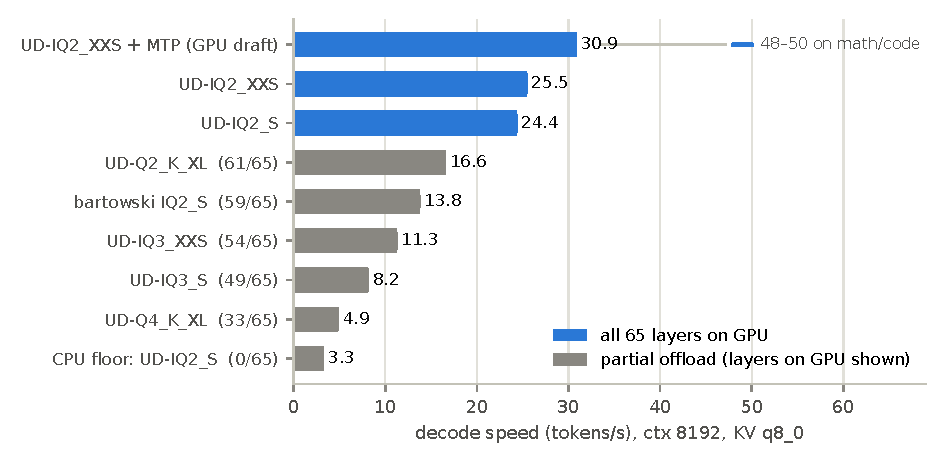
\includegraphics[width=\textwidth]{fig_ladder.pdf}
\caption{The measured speed ladder. Blue: all 65 layers GPU-resident; gray:
partial offload (GPU layer count in the label). The \q{UD-IQ2\_XXS}+MTP bar
shows prose decode; the whisker marks its measured 48--50\,tok/s on
math/code content (\S\ref{sec:mtp}). All base bars use the same
\q{llama-bench} tg128 protocol; the MTP annotations are separate server
measurements.}
\label{fig:ladder}
\end{figure}

Table~\ref{tab:phase1} and Figure~\ref{fig:ladder} give the matrix. The
full-residency boundary is the dominant feature; nominal labels and prompt
processing add two important qualifications.

\paragraph{For llama.cpp/GGUF, the full-GPU boundary lies between 7.8 and
9.2\,GiB in this run state.}
With the desktop session holding $\sim$900\,MiB, only the 6.8 and 7.8\,GiB
artifacts fit all 65 layers. Everything larger sheds layers to system RAM and
slows immediately. Within the GGUF ladder, footprint and consequent residency
are the first-order predictors of speed. This boundary is engine-specific:
ExLlamaV3 later fits a 9.50\,GiB EXL3 checkpoint (\S\ref{sec:exl3}).

\paragraph{The nominal quant label does not determine footprint or speed.}
Unsloth's \q{UD-IQ2\_S} (7.8\,GiB, 2.49 effective bpw) runs 24.4\,tok/s;
bartowski's \q{IQ2\_S} (9.6\,GiB, 3.06 effective bpw) runs 13.8\,tok/s. The
files share a nominal label but not a size, tensor allocation, or packaging:
the bartowski file also embeds MTP tensors. The observed speed difference is
consistent with full versus partial residency; it does not isolate a
quant-maker or allocation effect.

\paragraph{At 512 prompt tokens, GPU-heavy configurations ingest much faster
than they decode.} The controlled pp512 rates were 360--733\,tok/s, while the
CPU-only i-quant floor fell to 4.1\,tok/s. These short-context microbenchmarks
must not be extrapolated to 32K prompts; the deadline behavior in
\S\ref{sec:exl3} shows why.


\subsection{Offload Decay Follows a Two-Bandwidth Model}
\label{sec:offload}

\begin{figure}[t]
\centering
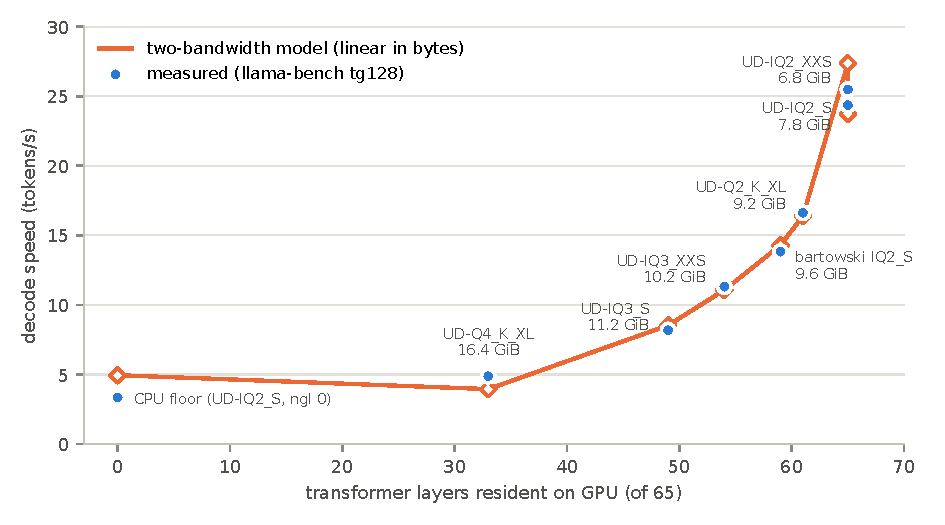
\includegraphics[width=\textwidth]{fig_offload.pdf}
\caption{Decode speed vs.\ GPU-resident layer count (blue, measured), with the
two-bandwidth model's per-config predictions (orange). The model, fitted for
relative error over all eight points, is
$1/\text{tok/s} = b_{\text{GPU}}/199\,\text{GB/s} +
b_{\text{CPU}}/41\,\text{GB/s}$ where $b$ are resident byte counts
(file bytes split proportionally to layers). The six non-extreme measured
states land within $\pm 8\%$; the two extremes' deviations are consistent with a
quant-family-dependent CPU term (i-quants dequantize expensively on CPU, so the ngl-0
floor runs $32\%$ below the pure-bandwidth prediction, while k-quant
\q{UD-Q4\_K\_XL} runs $24\%$ above it).}
\label{fig:offload}
\end{figure}

Figure~\ref{fig:offload} tests the bandwidth model of \S\ref{sec:hw} against
the matrix. Per-token time is linear in the two resident byte counts, with
fitted effective path bandwidths of \textbf{199\,GB/s} (GPU-resident bytes)
and \textbf{41\,GB/s} (CPU-resident bytes) --- a $4.9\times$ ratio, and the
reason each shed layer costs so much.
The fit's residual structure is itself informative: deviations concentrate
where CPU dequantization cost differs by quant family, i.e., the ``linear in
bytes'' rule needs a per-family CPU coefficient before it can be used
predictively across formats. For ranking configs on one family it is already
accurate to a few percent.


\subsection{MTP Benefit Depends on Workload and Placement}
\label{sec:mtp}

On the controlled prose prompt, the MTP draft head increased decode throughput by
21\% (25.5 $\rightarrow$ 30.9\,tok/s) at temperature 1.0 with the draft fully
on GPU, at a 41\% acceptance rate. During the MATH run, the same deployed
configuration produced 45--50 output tokens/s. That higher workload rate is
consistent with greater acceptance on structured text, but no draft-off run was
collected on the identical MATH prompts, so it is not a controlled 90\% MTP
effect. Likewise, the 9.6\,s mean GSM8K item time for
\q{UD-IQ2\_XXS}+MTP versus 17.7\,s for \q{UD-IQ2\_S} is a deployment
comparison, not an isolated MTP comparison: both the artifact and draft setting
change.

Two operational caveats. First, with the draft on CPU, MTP was a \emph{loss}
($-16\%$) or a wash in the controlled prose runs; these results should not be carried
over to other sampling regimes. Second, the draft's
VRAM cost is treacherous: $\sim$2.8\,GiB GPU-side when GPU-hosted, and still
$\sim$\textbf{1.2\,GiB} when nominally CPU-hosted (\q{-ngld 0}), because its
context and compute buffers allocate on the GPU regardless. This silently
crashed every tightly fitted mid-size config in our first sweep (the
``crashed'' rows of Table~\ref{tab:phase1}) until the harness guard learned to
account for it.

The result is therefore configuration-specific: MTP can help substantially
when the draft fits on GPU, but it is neither free in VRAM nor described by one
workload-independent speedup.



\subsection{Easy-Suite Accuracy Screen}
\label{sec:phase2}
\label{sec:phase2a}

\begin{table}[t]
\centering
\small
\caption{GSM8K ($n{=}50$) and HumanEval (executed, $n{=}20$) at
reasoning-effort medium, with Wilson 95\% CIs. Correct/min $=$ number of
successful items divided by summed logged HTTP-response wall time (local
post-response scoring excluded); compare only within a suite.}
\label{tab:phase2a}
\begin{tabular}{lrllrr}
\toprule
Config & tok/s & GSM8K & HumanEval & \multicolumn{2}{c}{correct/min} \\
 & & & & GSM8K & HE \\
\midrule
\q{UD-IQ2\_XXS}+MTP & 30.9 ($\approx$49 math) & 96\% [86.5, 98.9] & 80\% [58.4, 91.9] & \textbf{6.01} & 1.66 \\
\q{UD-IQ2\_S} & 24.4 & 94\% [83.8, 97.9] & \textbf{100\%} [83.9, 100] & 3.18 & \textbf{1.67} \\
\q{UD-Q2\_K\_XL} & 16.6 & 94\% [83.8, 97.9] & 100\% [83.9, 100] & 2.26 & 1.53 \\
\q{IQ2\_S} (bartowski) & 13.8 & 98\% [89.5, 99.6] & 95\% [76.4, 99.1] & 2.21 & 1.05 \\
\q{UD-IQ3\_XXS} & 11.3 & 96\% [86.5, 98.9] & 100\% [83.9, 100] & 1.65 & 0.92 \\
\q{UD-IQ3\_S} & 8.2 & 98\% [89.5, 99.6] & 100\% [83.9, 100] & 1.23 & 0.70 \\
\q{UD-Q4\_K\_XL} & 4.9 & 98\% [89.5, 99.6] & 100\% [83.9, 100] & 0.66 & 0.42 \\
\bottomrule
\end{tabular}
\end{table}

Table~\ref{tab:phase2a} has little resolution among the larger artifacts:
GSM8K estimates span 94--98\%, and HumanEval estimates span 95--100\% above
2.16 effective bpw. \q{UD-IQ2\_XXS} has the lowest HumanEval estimate (80\%),
but all intervals are wide. The practical difference is time. Across these two
suites, \q{UD-Q4\_K\_XL} used $4.6\times$ the pooled wall-clock of
\q{UD-IQ2\_S} ($7318\,\text{s}/1606\,\text{s}$) and recorded two additional
successes out of 70; no accuracy difference was resolved. Because these older
suites cluster near the top of their scales, the next experiments use the fixed MATH-25
subset and HumanEval+ to seek greater separation.


\subsection{MATH Answer-Parser Sensitivity}
\label{sec:artifact}

The original MATH parser scored \q{UD-IQ2\_S} at 14/25 and
\q{UD-IQ3\_XXS} at 22/25. Inspection of the saved responses found rejected
strings that differed from the reference in answer tags, math delimiters,
Unicode symbols, degree notation, brace shorthand, or an equation such as
\q{x=5} where the key contained \q{5}.

After inspecting those failures, we wrote a deterministic alternate
normalizer and applied it to every saved prediction. It accepts the declared
equivalences, leaves truncations wrong, and leaves mechanically unresolved
cases wrong. Because the rules were chosen post hoc, this score is not an
independent measure of mathematical correctness and does not replace the
original deployment parser. Table~\ref{tab:math25} and
Figure~\ref{fig:artifact} report both scores, with the rules and retained
per-item scoring records available for audit. No inference was rerun for this
analysis.

\begin{table}[t]
\centering
\small
\caption{MATH-25 ($n{=}25$, competition level 4--5): original parser score
vs.\ alternate-normalizer score, with the number of upgraded items
(value-equivalent under the alternate rules) and truncations (8K generation
budget exhausted; wrong under both scorers). Wilson 95\% CIs use the alternate
score. Reasoning-effort medium except where noted. Two \q{UD-Q4\_K\_XL} rows
lost their ground-truth field to a harness bug; the rescorer recovers them from
the dataset.}
\label{tab:math25}
\setlength{\tabcolsep}{5pt}
\begin{tabular}{lrrlcc}
\toprule
Config (eff.\ bpw) & Original & Alternate & CI (alternate) & Upgraded & Trunc. \\
\midrule
\q{UD-IQ2\_XXS}+MTP (2.16) & 12/25 & 16/25 (64\%) & [44.5, 79.8] & 4 & 3 \\
\q{UD-IQ2\_S} (2.49) & 14/25 & \textbf{23/25 (92\%)} & [75.0, 97.8] & \textbf{9} & 1 \\
\q{UD-IQ2\_S}, xhigh (2.49) & 17/25 & 21/25 (84\%) & [65.3, 93.6] & 4 & 4 \\
EXL3 2.0\,bpw (3.03) & 20/25 & \textbf{24/25 (96\%)} & [80.5, 99.3] & 4 & 1 \\
\q{IQ2\_S} bartowski (3.06) & 20/25 & 23/25 (92\%) & [75.0, 97.8] & 3 & 1 \\
\q{UD-IQ3\_XXS} (3.25) & 22/25 & \textbf{24/25 (96\%)} & [80.5, 99.3] & 2 & 0 \\
\q{UD-Q4\_K\_XL} (5.22) & 18/25 & 23/25 (92\%) & [75.0, 97.8] & 5 & 0 \\
\bottomrule
\end{tabular}
\end{table}

\begin{figure}[t]
\centering
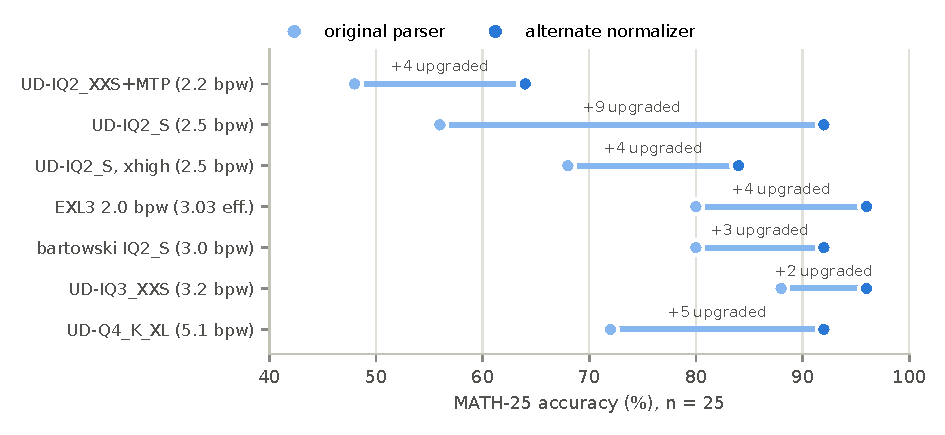
\includegraphics[width=\textwidth]{fig_artifact.pdf}
\caption{Original$\rightarrow$alternate score changes on MATH-25 ($n{=}25$).
The connector shows how many responses the post-hoc normalizer accepts that
the original parser rejected; both endpoints remain visible because the
rescore is not independent ground truth. The largest change is 9/25 at 2.49 effective bpw, versus
2/25 at 3.25 effective bpw.}
\label{fig:artifact}
\end{figure}

\paragraph{Accuracy across artifacts.}
Under the post-hoc normalizer, the estimates from 2.49 to 5.22 effective bpw
are 92--96\% and are not resolved from one another at this sample size. The
2.16-effective-bpw artifact scored 16/25, compared with 23/25 at 2.49 bpw on
the same items: seven successes favored the 2.49-bpw artifact and none favored
2.16 bpw (paired exact $p{=}0.016$, exploratory and uncorrected). No GGUF was
tested between 2.16 and 2.49 effective bpw, so the experiment identifies a
difference between these artifacts, not a universal threshold.

\paragraph{Parser sensitivity.}
For \q{UD-IQ2\_S}, the post-hoc normalizer accepted 9/25 responses rejected by
the original parser; for \q{UD-IQ3\_XXS}, it accepted 2/25. On the paired
items, seven changed only for IQ2\_S and none only for IQ3\_XXS (exact
$p{=}0.016$, exploratory and uncorrected). This establishes that parser
acceptance changed the apparent gap unevenly in these saved outputs. It does
not establish that every newly accepted response is semantically correct, or
that quantization generally harms answer formatting before reasoning.
Parser-compatible output remains a real deployment capability, so both scores
are retained.

\paragraph{Execution-scored code.} Generated code is
extracted from a fenced block and then executed, so it avoids symbolic-answer
normalization but still treats a missing/malformed code block as failure. We did
not post-hoc rescore those format failures; Table~\ref{tab:hard} reports the
end-to-end parser and test outcome as deployed.


\subsection{Hard-Suite Accuracy}
\label{sec:phase2b}

\begin{table}[t]
\centering
\small
\caption{Hard-suite summary (reasoning-effort medium). HumanEval+ is
execution-scored ($n{=}20$), Wilson 95\% CIs. Correct/min uses the
alternate MATH-25 score and each run's summed logged HTTP-response wall time;
post-response parsing and code execution are excluded.
The xhigh HumanEval+ entry is the truncation-free re-run
(\S\ref{sec:effort}).}
\label{tab:hard}
\setlength{\tabcolsep}{4pt}
\begin{tabular}{lllrr}
\toprule
Config (eff.\ bpw) & MATH-25 (alternate) & HumanEval+ & \multicolumn{2}{c}{correct/min} \\
 & & & math & HE+ \\
\midrule
\q{UD-IQ2\_XXS}+MTP (2.16) & 64\% [44.5, 79.8] & 70\% [48.1, 85.5] & 0.69 & 1.99 \\
\q{UD-IQ2\_S} (2.49) & 92\% [75.0, 97.8] & 90\% [69.9, 97.2] & 0.73 & 1.40 \\
\q{UD-IQ2\_S}, xhigh (2.49) & 84\% [65.3, 93.6] & 80\% [58.4, 91.9] & 0.37 & 0.73 \\
EXL3 2.0\,bpw (3.03) & \textbf{96\%} [80.5, 99.3] & 90\% [69.9, 97.2] & \textbf{0.83} & \textbf{2.27} \\
\q{IQ2\_S} bartowski (3.06) & 92\% [75.0, 97.8] & 90\% [69.9, 97.2] & 0.38 & 0.86 \\
\q{UD-IQ3\_XXS} (3.25) & \textbf{96\%} [80.5, 99.3] & 90\% [69.9, 97.2] & 0.33 & 0.73 \\
\q{UD-Q4\_K\_XL} (5.22) & 92\% [75.0, 97.8] & \textbf{95\%} [76.4, 99.1] & 0.19 & 0.43 \\
\bottomrule
\end{tabular}
\end{table}

Table~\ref{tab:hard} collects the hard suites. The 2.16-effective-bpw artifact
has the lowest point estimate on both: 16/25 alternate MATH and 14/20
HumanEval+, compared with 23/25 and 18/20 for the 2.49-bpw artifact. Because
every configuration saw the same items, paired tests are appropriate. The
MATH comparison has seven IQ2\_S-only successes and no IQ2\_XXS-only successes
(exact two-sided $p{=}0.016$); HumanEval+ has four and zero, respectively
($p{=}0.125$). Thus these data resolve the MATH loss but not the code-suite
difference. We do not pool the two suites into a single significance test.

Above 2.16 effective bpw, alternate MATH estimates are 92--96\% and HumanEval+
estimates are 90--95\%; no difference is resolved at these sample sizes. That
is evidence for a plateau within this experiment, not proof that the artifacts
or formats are equivalent. It also reinforces why nominal ``2-bit'' is too
coarse a label: the evaluated files bearing it span 2.16--3.06 effective bpw
and produced materially different hard-suite point estimates.


\subsection{Matched-Footprint Deployment Comparison}
\label{sec:exl3}

The EXL3 checkpoint is labeled 2.0\,bpw, but its 9.50\,GiB weight-file total is
\textbf{3.03 effective bpw}: the transformer weights target roughly 2\,bpw,
while the output head is 3-bit and other tensors are wider. It therefore is
not a footprint-matched comparison with the 6.77\,GiB, 2.16-effective-bpw
GGUF. Crediting their quality difference to trellis coding would confound
method with 40\% more effective bits.

The direct footprint control is bartowski \q{IQ2\_S}: 9.59\,GiB and 3.06
effective bpw. On identical hard-suite subsets, EXL3 scored 24/25 versus 23/25
on alternate MATH and both scored 18/20 on HumanEval+. These small samples do
not resolve a quality difference. They do expose a deployment difference: the
EXL3--ExLlamaV3 stack was fully GPU-resident, whereas the
bartowski-GGUF--llama.cpp stack offloaded six of 65 units. From the server logs
on these same workloads,
token-weighted generation throughput was 22.4 versus 13.7\,tok/s on MATH
($1.64\times$) and 30.7 versus 13.8\,tok/s on HumanEval+ ($2.22\times$).
The rate varies with output length and workload, so we use the MATH result as
the headline comparison: \textbf{at matched footprint, the fully resident
EXL3 deployment generated $1.6\times$ faster, and the available hard-suite
samples did not resolve a score difference.}

The other measured comparisons clarify what this result does and does not
identify:

\begin{itemize}
  \item At similar effective bpw, EXL3 (3.03) and \q{UD-IQ3\_XXS} (3.25)
  both scored 24/25 on alternate MATH and 18/20 on HumanEval+. We measured no
  quality-per-effective-bit advantage for either artifact at this point.
  \item Against \q{UD-IQ2\_XXS} (2.16), EXL3 has higher point scores but also
  a 2.73\,GiB larger file. This experiment cannot locate a trellis-specific
  quality boundary near 2.2 effective bpw.
\end{itemize}

This is the concrete sense in which the 12\,GB system exceeded a naive
capacity-based expectation: a 9.50\,GiB checkpoint remained resident and ran
at useful speed, while a nearly identical-size GGUF offloaded weights to RAM.
Because format and engine changed together, the experiment compares complete
deployments and cannot attribute the difference to trellis coding alone.

\begin{table}[t]
\centering
\small
\caption{Selected-deployment validation. MMLU used the same fixed 200-item,
57-subject-stratified subset; CIs are Wilson 95\%. Correct/min uses logged
HTTP-response wall time (post-response scoring excluded). Needle reports
probes completed correctly
before the client exhausted two 600-s HTTP attempts (one automatic retry),
not pure retrieval accuracy.}
\label{tab:validation}
\setlength{\tabcolsep}{5pt}
\begin{tabular}{lrrrl}
\toprule
Config & MMLU & Mean wall/item & Correct/min & Needle deadline success \\
\midrule
\q{UD-IQ2\_S} & 175/200, 87.5\% [82.2, 91.4] & 36.41\,s & 1.44 & 4/6 [30.0, 90.3] \\
EXL3 2.0\,bpw & 182/200, 91.0\% [86.2, 94.2] & 25.42\,s & 2.15 & 6/6 [61.0, 100] \\
\bottomrule
\end{tabular}
\end{table}

On paired MMLU items, both were correct on 171, only \q{UD-IQ2\_S} on four,
only EXL3 on 11, and neither on 14 (exact two-sided McNemar $p{=}0.119$).
The 3.5-point estimate therefore does not resolve a quality difference, while
EXL3 returned more correct items per minute. On the needle probes,
\q{UD-IQ2\_S} answered all four 8K/16K contexts but its two 32K items produced
no answer after two 600-s HTTP attempts each (one automatic retry after a
2-s delay, or about 1,202\,s total per item); EXL3 completed all six. The
4/6 versus 6/6 count measures completion under this client policy and includes
a large prompt-processing difference, so it must not be read as two wrong
retrieval answers.


\subsection{Reasoning-Effort Check}
\label{sec:effort}

Qwen3.8's chat template exposes a \q{reasoning\_effort} dial. For
\q{UD-IQ2\_S}, xhigh produced no observed benefit. On MATH-25 it scored
21/25 (84\%) under the alternate normalizer versus 23/25 (92\%) at medium,
with four rather than one 8K truncations. Mean wall time rose from 75.89 to
134.44\,s per item ($1.77\times$). On HumanEval+, an initial xhigh run was
truncation-confounded; the 8K-budget re-run removed truncations and scored
16/20 (80\%) versus 18/20 (90\%) at medium. Neither accuracy difference is
resolved at this sample size. The useful conclusion is narrower: xhigh was
slower and did not improve either point estimate in these runs, so medium is
the better measured setting for this deployment. This is not evidence that
additional reasoning effort is generally harmful.



\subsection{Correct Responses per Minute at Fixed VRAM}
\label{sec:metric}

\begin{figure}[t]
\centering
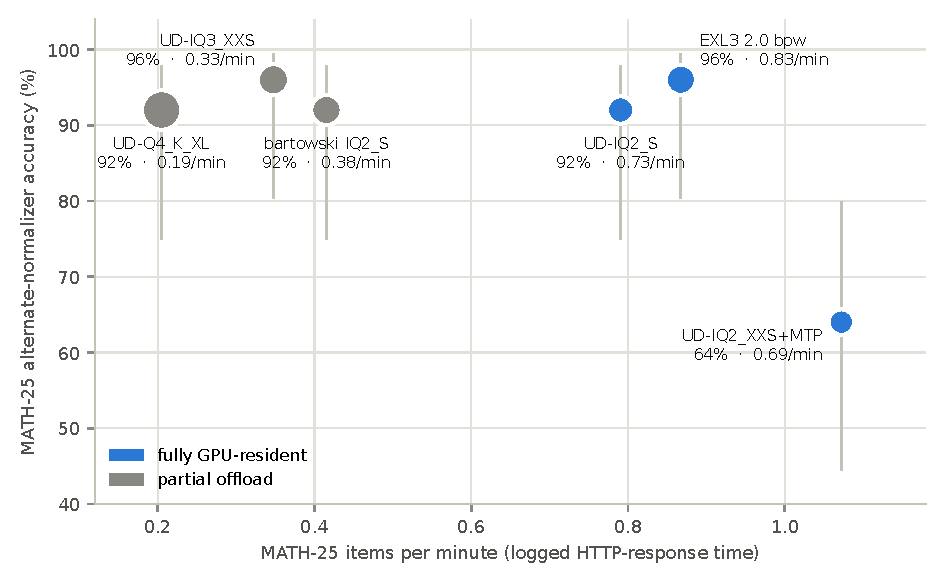
\includegraphics[width=\textwidth]{fig_frontier.pdf}
\caption{MATH-25 point estimates using logged HTTP-response time.
$x$: benchmark items completed per minute, whether correct or not; $y$:
alternate-normalizer accuracy with Wilson 95\% intervals; point area
$\propto$ file GiB. Their product is correct responses per minute. Colors
encode the measured residency state. The vertical intervals overlap widely;
the plot compares observed deployment rates and does not establish quality
dominance.}
\label{fig:frontier}
\end{figure}

For a fixed suite, correct responses per minute is the number scored correct
divided by summed per-item HTTP-response wall time. The timer includes prompt
processing, generation, retries, and request overhead, but stops before local
post-response parsing or code execution. It answers a deployment question---
how many successful model responses this machine returned per minute---without
pretending that a correct MATH item and a correct HumanEval+ item have the same
value. We therefore compare it only within a suite and always print the
underlying accuracy beside it.

The response-time view in Figure~\ref{fig:frontier} avoids the cross-engine
token/s problem: it prices prompt processing, generation length, retries,
request overhead, MTP, and offload as logged. It does not price local scoring.
On MATH-25, EXL3 has the highest observed
correct/min (0.83), followed by fully resident \q{UD-IQ2\_S} (0.73) and the
faster but less accurate \q{UD-IQ2\_XXS}+MTP (0.69). The partial-offload
artifacts range from 0.19 to 0.38. On HumanEval+, EXL3 has the highest
observed rate at 2.27, followed by the faster but lower-scoring
\q{UD-IQ2\_XXS}+MTP at 1.99 and \q{UD-IQ2\_S} at 1.40. These are efficiency
estimates on the observed subsets, not statistically distinct quality
rankings or a recommendation that ignores error cost.


\section{Discussion}
\label{sec:discussion}

\subsection{Deployment Recommendations}

For this machine, the measurements support distinct deployment choices.
Extrapolation to
other 12\,GB systems requires repeating the fit search because desktop VRAM,
engine buffers, and memory bandwidth change the boundary.

\begin{enumerate}
  \item \textbf{Default when the ExLlamaV3 stack is suitable: EXL3
  2.0\,bpw (3.03 effective).} It has the highest measured hard-suite
  correct/min and, among the two configurations selected for validation, the highest MMLU
  correct/min, with no resolved quality difference from the larger tested
  anchors. Its speed advantage is workload-dependent, and this run did not
  configure MTP or vision.
  \item \textbf{GGUF all-rounder: \q{UD-IQ2\_S}.} It remains fully resident,
  scored 92\%/90\% on the hard suites, and uses the llama.cpp/GGUF stack. The
  separate unsloth MTP draft did not fit in the measured desktop run state.
  \item \textbf{Maximum throughput when errors are cheaper:
  \q{UD-IQ2\_XXS}+MTP.} It delivered the fastest measured generation and
  6.01 correct GSM8K items/min, but its 64\% alternate MATH and 70\%
  HumanEval+ estimates were lower than the resident alternatives. It is not
  the recommendation for correctness-sensitive work.
\end{enumerate}


\subsection{Research Directions}

These measurements motivate a broader systems hypothesis: under a fixed VRAM
budget, useful single-stream throughput is often maximized by a deployment
that sits above the task-accuracy loss boundary but below the engine's
offload boundary. The present experiment establishes one instance, not a
general law. Testing the hypothesis requires repeating the same fit--speed--
accuracy map across models, engines, 8/12/16/24\,GB memory budgets, context
lengths, and power limits.

The highest-priority quality extension is a bf16, Q8, or hosted reference run
on hardware large enough to hold it. That would determine how much accuracy
all tested 12\,GB deployments lose relative to the original model; the current
Q4 anchor only supports comparisons within this experiment. Denser sampling
between 2.16 and 2.49 effective bpw, larger hard-task sets, and repeated
generations would test whether the observed GGUF drop is stable.

A method-level EXL3 claim would require tighter controls over tensor
precision, packaged components, kernels, and memory allocation, ideally with
one engine supporting both representations. The MATH audit can be strengthened
without rerunning inference: an independent, preregistered human or
computer-algebra review can rescore the archived predicted-answer fields. New inference
runs would be needed to estimate run-to-run variability or test whether
parser compatibility changes systematically with quantization.

\section{Limitations and Threats to Validity}
\label{sec:limitations}

\begin{itemize}
  \item \textbf{No unquantized quality reference.} We did not evaluate bf16,
  Q8, or the hosted model. Comparisons to \q{UD-Q4\_K\_XL} rank only the
  tested artifacts and do not establish parity with the original model.
  \item \textbf{Limited statistical power.} MATH-25 and HumanEval+ contain
  only 25 and 20 fixed items. Their Wilson intervals are wide; a non-significant
  comparison is not evidence of equality. MMLU is larger but tests a different
  capability mix. No correction was applied across the exploratory paired
  comparisons.
  \item \textbf{One stochastic sample.} Each item was generated once at
  temperature 1.0. The intervals quantify item sampling only, not variation
  across repeated generations.
  \item \textbf{Post-hoc alternate scoring.} The MATH normalizer was written
  after failures were inspected. Publishing its rules, retained per-item
  scoring records, original scores, and alternate scores makes the judgment
  auditable but does not make
  it independent or pre-registered.
  \item \textbf{Deployment, not method isolation.} The EXL3--GGUF comparison
  changes format, artifact, kernels, memory allocation, and engine together.
  It supports a choice between the tested deployments, not a causal claim
  about trellis coding.
  \item \textbf{Speed protocols.} The GGUF ladder uses controlled tg128 runs;
  no matching EXL3 microbenchmark was collected. Cross-engine ratios in
  \S\ref{sec:exl3} instead use engine-reported generation metrics on the same
  evaluation workloads. Correct/min uses logged HTTP-response wall time and is
  the more comparable deployment measure; it excludes local scoring time.
  \item \textbf{Scope and provenance.} Results come from one model, laptop,
  run state, and set of artifacts downloaded on one date. File sizes identify
  the local artifacts. Upstream revisions were recovered from the local cache
  after the campaign rather than emitted into the measurement logs at run
  time; the release records those revisions together with the exact file
  SHA-256 values. The 80\,W power limit is not an energy measurement, and no
  sustained thermal or per-watt conclusion is reported.
  \item \textbf{Long-context timeout contamination.} The two failed 32K
  \q{UD-IQ2\_S}+llama.cpp probes exhausted both 600-s HTTP attempts without
  returning an answer, so the needle comparison combines prompt-processing
  speed with retrieval behavior.
\end{itemize}



\section{Related Work}
\label{sec:related}

\textbf{Quantization methods.} This work evaluates existing post-training
quantization rather than introducing a method: GGUF k/i-quants in llama.cpp
\citep{gerganov2023llamacpp}, dynamic mixed-tensor GGUF recipes
\citep{unsloth2026dynamic}, and EXL3 \citep{turboderp2025exllamav3}, whose
trellis construction builds on QTIP \citep{tseng2024qtip}. GPTQ (published at
ICLR as OPTQ)
\citep{frantar2022gptq}, AWQ \citep{lin2023awq}, and ParetoQ
\citep{liu2025paretoq} provide broader calibration and low-bit scaling context.
Our effective-bpw accounting is a deployment-footprint measure, not a new
quantization metric.

\textbf{Post-freeze update (checked 2026-08-29).}
On 2026-08-28, after our 2026-08-25 artifact freeze, ISTA-DASLab released
Qwen3.8-27B checkpoints that use GSQ for low-bit scalar quantization and RCO
for per-tensor GGUF-type assignment under a file-size budget
\citep{dadgarnia2026gsq,helcig2026rco,istadaslab2026qwen38gsqrco}. They are
standard GGUF files, not a GSQ/RCO-specific runtime modification; we did not
evaluate their quality, residency, or correct/min on this system.

\textbf{Evaluation and answer parsing.} Prior work shows that aggregate task accuracy
can conceal important changes under quantization \citep{dutta2024accuracy},
and low-bit mathematical reasoning has been studied through process and error
taxonomies \citep{quantreasoning2025,extremelowbit2026}. Separately, structured
output research distinguishes semantic correctness from machine usability
\citep{correctnotusable2026}, while evaluation scaffolding can materially alter
measured outcomes \citep{scaffolding2026}. Task difficulty and instruction
following also interact with quantization \citep{quantinstruct2024}. Our
MATH audit is a small, concrete instance of these broader warnings: a
post-hoc alternate normalizer changed the apparent low-bit gap, so the
original-parser and post-hoc-normalized scores must remain visible. Community measurements that report strict or
machine-usable output rates provide a related operational view
\citep{strix2026}.

\textbf{Extreme-low-bit and cross-format comparisons.} Bielik-Q2-Sharp
compares six academic extreme-2-bit methods on an 11B Polish model and finds
that rankings depend on method and summary metric \citep{bielik2026q2sharp}.
Broader unified GGUF evaluation reports FP16, size, perplexity, throughput, and
standard downstream tasks on Llama-3.1-8B \citep{kurt2026whichquant}; a
contemporaneous Qwen3.8-27B study compares bf16 through 1-bit GGUFs on larger
datacenter GPUs \citep{migdal2026qwen38}. Those studies provide wider precision
or task coverage; the present question is the realized 12\,GB deployment
boundary.
EXL3's documentation reports its own quality curves
\citep{turboderp2025exllamav3}; an earlier matched-bpw community comparison
reported lower MMLU for lower-bpw EXL2 variants than for GGUF at matched
quantized-layer bpw on Llama~3 \citep{mattc1llama3}. Our data should not be
read as a method-level reversal of either result. At roughly 3 effective bpw we
resolve no hard-suite quality difference; the contribution is a matched-file-
footprint deployment comparison in which the EXL3 artifact remains resident
and the GGUF control does not.

\textbf{Local inference under resource constraints.} Bench360 evaluates
quality, latency, energy, and Pareto tradeoffs under a fixed 24\,GB budget
\citep{bench360}; other work studies accuracy--performance tradeoffs on server
GPUs \citep{kurtic2024bf16}, joint performance, energy, and quality under
online GPU serving \citep{qmeter2025}, and various combinations of latency,
quality, and energy on mobile, edge, or private-server systems
\citep{sustainableedge2025,palmbench2024,privateserver2025}. Silicon Showdown describes the consumer ``VRAM wall'' and
the throughput cost of CPU offload \citep{javat2026siliconshowdown}, while
pipelined sub-layer sharding targets that cost with a new client inference
system \citep{ukarande2026vram}.

Most directly, Moreira reports Qwen3.8-27B on a 12\,GB RTX~4070~Ti: a fully
resident IQ2 configuration generated at 43.643 tokens/s versus 5.977 for a
partially offloaded IQ4\_XS, while a 24-item custom suite favored IQ4\_XS
13--9 without resolving the paired difference \citep{moreira2026qwen38}.
Its desktop hardware, artifact, runtime, context, and speed protocol differ
from ours, so those absolute rates are prior evidence about the fit--offload
trade rather than a throughput baseline for this study.
Thus our study is not the first task-level fit-versus-offload measurement for
this model and memory class. It contributes an independent 80\,W laptop
characterization with standard task families, effective-footprint and
engine-residency accounting, a matched-footprint EXL3/GGUF deployment pair,
and an explicit parser audit. Correct/min is a descriptive within-suite
task-goodput rate, not a proposed universal or novel benchmark.

Our MTP measurements are an instance of speculative decoding
\citep{leviathan2022speculative,chen2023speculative}; they do not evaluate
speculative-decoding algorithms themselves.


\section{Artifact Availability and Reproducibility}
\label{sec:repro}

Every reported result traces to archived JSONL data alongside the harness:
\begin{itemize}
  \item fit searches, \q{llama-bench} results, timings, and VRAM peaks in
  \path{testsuite/results/phase1.jsonl};
  \item per-suite summaries in
  \path{testsuite/evals/results/summary.jsonl}; and
  \item per-item JSONL scoring records in each retained configuration's
  results directory, including predicted and expected answer fields and the
  final 200 characters of each saved response where applicable.
\end{itemize}
The alternate MATH-25 numbers come from the deterministic $\sim$50-line
\path{testsuite/evals/rescore_math25.py}; every rule is listed in
\S\ref{sec:artifact}. Figures are generated directly from these logs by
\path{paper/scripts/make_figures.py}. Engine server logs preserve the per-request
metrics used for the matched-workload comparison.

Software: llama.cpp master \q{b1-1729ed5}, CUDA 12.6.3 (user-local
toolchain), SM 8.9, flash-attn on; ExLlamaV3 1.4.3 under TabbyAPI
(\q{max\_seq\_len} 16384 for the main hard suites and 36864 for validation).
Artifacts: unsloth \q{Qwen3.8-27B-GGUF} UD tier,
bartowski \q{Qwen3.8-27B-GGUF} \q{IQ2\_S}, turboderp EXL3 \q{SC\_2.00bpw\_H3}
all downloaded 2026-08-25. File sizes in Table~\ref{tab:artifacts} identify
the local artifacts; the release manifest records every tested upstream
revision, filename, byte count, and SHA-256. Evaluation ran through each
engine's OpenAI-compatible endpoint; \q{reasoning\_effort} was passed per
request via \q{chat\_template\_kwargs}. Harness safety rules (VRAM fit guard
including the 1.2\,GiB \q{-ngld 0} draft-buffer correction, mmap-backed CPU
weights, one model process at a time) are documented in the harness and were
calibrated against the measured peaks in Table~\ref{tab:phase1}.

The public artifact should be used in two modes: an analysis-only path that
rebuilds tables and figures from archived logs without launching inference,
and a prospective replication path that downloads the pinned model artifacts
and reruns the GPU harness. The accompanying artifact includes a paper-specific README,
environment and hardware requirements, model revisions and checksums, concrete
setup and launch commands, expected outputs, and an immutable tag or archive
identifier. The version-of-record compendium is archived at
\href{https://doi.org/10.5281/zenodo.22166977}{doi:10.5281/zenodo.22166977};
the matching tagged source and results tree is
\url{https://github.com/matthematics1137/research-artifacts/tree/qwen38-27b-12gb-v1.0.0/papers/2026-qwen38-27b-12gb}.
The ML-facing result dataset is
\url{https://huggingface.co/datasets/mv1137/qwen38-27b-12gb-results}.
Full response transcripts were not retained: the per-item files contain scoring fields and
short answer excerpts. The Q4 easy-suite runs also lack per-item GSM8K and
HumanEval files and are supported only by their frozen aggregate summary rows.
We preserve these gaps rather than reconstructing records after the fact.


\section{Conclusion}

On the tested 12\,GB laptop, the best measured way to run Qwen3.8-27B was not
to load the largest artifact possible and accept CPU offload. Fully resident
GGUFs decoded at 24--25 tokens/s, while progressively offloaded GGUFs fell to
16.6--4.9 tokens/s. A 9.50\,GiB EXL3 checkpoint remained resident under
ExLlamaV3; compared with a 9.59\,GiB GGUF under llama.cpp, it generated
$1.6\times$ faster on MATH, had no hard-suite score difference resolved at the
available sample sizes, and produced the highest observed correct responses
per minute on MATH and HumanEval+.

The practical result is that this 12\,GB system ran a 27.4B model without the
repeated RAM weight reads that dominated the larger GGUF deployments. Finding
that operating point required the actual checkpoint footprint, engine memory
behavior, GPU residency, response time, and answer parser; the advertised bit
label alone was insufficient. This experiment does not establish parity with
bf16 or Q8, a universal optimum, or a trellis-specific advantage. Broader
claims require larger repeated evaluations, an unquantized or near-lossless
reference, and replication across models, engines, and memory budgets.

\medskip
\noindent\textbf{AI assistance.} Claude (Anthropic) and Codex (OpenAI) assisted
with evaluation-harness development, experiment execution, evidence auditing,
analysis and figure code, and manuscript drafting and revision. Matthew
Schwartz directed the work, reviewed and verified the retained outputs against
the archived evidence and cited sources, edited the manuscript, and takes full
responsibility for the methods, results, interpretation, citations, and
released artifacts.

\bibliographystyle{unsrtnat}
\bibliography{references}

% ===========================================================================

\end{document}
.
% When ON: near-black blue-warm page, light-gray body text (never pure white,
% to avoid halation), brighter section heads, soft cyan/amber links, salmon
% figures/dark/ (generated by scripts/make_figures.py --dark).
\newif\ifdarkmode
\ifdefined\DARKMODE
  \darkmodetrue
\else
  \darkmodefalse
\fi

\ifdarkmode
  % Visual definitions shared with explainer.tex (pure extraction, no
  % behavior change): colors, \pagecolor, default-color patch, \hypersetup,
  % bright section heads.
  \input{darkstyle}
  \graphicspath{{figures/dark/}}
\else
  \graphicspath{{figures/}}
\fi
% ---------------------------------------------------------------------------


% Quant names appear constantly; keep them readable.
\newcommand{\q}[1]{\texttt{#1}}
\newcommand{\singleauthorinfo}[1]{\\[0.25em]{\small #1}}

\title{\textbf{Deploying Qwen3.8-27B in 12\,GB of VRAM: Accuracy and
Throughput Across Quantized Inference Stacks}}

\hypersetup{
  pdftitle={Deploying Qwen3.8-27B in 12 GB of VRAM: Accuracy and Throughput Across Quantized Inference Stacks},
  pdfauthor={Matthew Schwartz},
  pdfsubject={Quantized large-language-model inference under a 12 GB GPU memory budget}
}

\author{Matthew Schwartz\singleauthorinfo{Independent researcher \enspace
\href{https://orcid.org/0009-0009-4171-7247}{ORCID 0009-0009-4171-7247}
\enspace \texttt{matthew.schwartz.research@gmail.com}}}

\date{August 29, 2026}

\begin{document}
\maketitle

\begin{abstract}
\noindent
Quantized-inference studies usually report quality under a fixed engine or
throughput under a fixed quantization, but a 12\,GB GPU couples these choices:
weights, cache, and engine buffers must fit together, and spilled weights are
read from slower system RAM. We characterize this deployment problem for
Qwen3.8-27B on an 80\,W RTX 4080 Laptop GPU by measuring fit, throughput, and
task performance for eight artifacts across GGUF/llama.cpp and
EXL3/ExLlamaV3. Fully resident GGUFs decoded at 24.4--25.5 tokens/s, whereas
partial offload reduced decode to 16.6--4.9 tokens/s. At approximately
9.5\,GiB file footprint, EXL3/ExLlamaV3 remained fully resident while
GGUF/llama.cpp offloaded six of 65 units; the hard-suite samples did not
resolve an accuracy difference, but EXL3 generated $1.6\times$ faster on MATH
and achieved the highest observed correct responses per minute on MATH and
HumanEval+. Across GGUF, the 2.16-effective-bpw artifact lost seven paired
MATH items relative to the 2.49-effective-bpw artifact, while configurations
from 2.49 to 5.22 effective bpw were not separated at these sample sizes; the
original MATH parser also disagreed with the post-hoc normalizer unevenly
across artifacts, so we report both scores separately. On this machine, joint
artifact--engine selection kept a 27.4B model in 12\,GB of VRAM and delivered
correct responses faster than partial offload, with no hard-task difference
resolved relative to the largest tested artifact; we did not test bf16 or Q8,
or isolate engine from format.
\end{abstract}



\section{Introduction}
\label{sec:intro}

Quantized-inference work usually reports either quality under a fixed engine or
throughput under a fixed quantization. A 12\,GB discrete GPU couples the two:
the file, cache, and engine buffers must fit together, and crossing that boundary
moves weight reads from high-bandwidth VRAM to much slower system RAM. The
practical question is therefore not simply ``which quant has the best quality?''
It is: \emph{which artifact--engine pair returns correct answers fastest inside
this fixed memory budget?}

We answer that question for Qwen3.8-27B, whose 27.36 billion non-MTP VLM
parameters would require roughly 54.7\,GB at bf16 before runtime overhead, on
one 12\,GB laptop GPU. In
the measured run state, the right low-bit artifact and engine kept the model
fully GPU-resident. Its scores on the small hard-task suites were not resolved
from those of the largest tested artifact, and it returned more correct answers
per minute than the larger deployments that placed weights in system RAM. This
is the paper's central result: the machine did more useful work with a smaller,
fully resident deployment than with the largest tested, partially offloaded
artifact, which kept only 33 of 65 offload units on the GPU. More useful work
here means more correctly scored responses per minute, not a resolved
raw-accuracy advantage.

We first found the maximum GPU-resident layer count and measured prompt and
decode throughput for a GGUF ladder. We then evaluated selected configurations
on easy and harder task subsets, inspected MATH scoring failures item by item,
added a GGUF control with nearly the same file footprint as EXL3, and compared
the two recommended deployments on MMLU and long-context probes. We report
nominal quantization, actual checkpoint size, GPU residency, task score, and
wall-clock response rate separately.

\paragraph{Contribution and scope.}
The primary contribution is an end-to-end deployment map for a 27.4B model
under a 12\,GB laptop-GPU memory budget. It connects checkpoint footprint and
engine-specific residency to controlled throughput, benchmark accuracy, and
correct responses per minute. Fully resident GGUFs decoded at 24--25 tokens/s,
whereas progressively offloaded GGUFs fell to 16.6--4.9 tokens/s. At matched
file footprint, EXL3/ExLlamaV3 remained resident and generated faster than
GGUF/llama.cpp without a resolved hard-suite score difference.

Two audits qualify that result. Nominal bit labels did not reliably predict
whole-checkpoint size, and the post-hoc MATH normalizer accepted some surface
forms that the original parser rejected. We therefore compare complete artifact--engine
deployments rather than attributing the cross-stack result to trellis coding,
and report the original-parser score beside a disclosed post-hoc-normalized
score. The latter is a rescore of saved outputs, not an independent semantic
ground truth.

The hard-suite subsets are small ($n{=}20$--$25$), every generation is a single
sample at temperature 1.0, and engine and format cannot be separated in the
cross-ecosystem comparison. Wilson 95\% intervals accompany every accuracy.
These data characterize the tested deployments; they do not establish model-
or hardware-class generalities (\S\ref{sec:limitations}).


\section{Experimental Setup}
\label{sec:setup}

\subsection{Hardware}
\label{sec:hw}

All measurements were taken on a single consumer laptop: NVIDIA GeForce RTX
4080 Laptop GPU (Ada Lovelace, SM~8.9), 12{,}282\,MiB VRAM, capped at
\textbf{80\,W}; Intel Core i9-14900HX CPU; 62\,GiB dual-channel DDR5; NVMe
storage; Linux 7.0.0, driver 580.167.08. The desktop session held
$\sim$900\,MiB of VRAM, leaving a measured working envelope of roughly
10.5--11\,GiB for weights, cache/state, and compute buffers. Power mode, memory
clock, and sustained device clocks were not separately logged; the throughput
results therefore describe this run state, not a normalized hardware limit.

Batch-one dense decode is usually memory-bandwidth-bound: each generated
token's forward pass uses the active weight set, which is too large to remain
in on-chip cache, so memory traffic scales approximately with active weight
bytes and $\text{tok/s} \approx
\text{effective bandwidth}/\text{bytes per token}$. The laptop's GDDR6 is
$\sim$432\,GB/s on paper; our fitted effective GPU-resident weight-path
bandwidth is 199\,GB/s (\S\ref{sec:offload}). The fitted CPU-resident
weight-path coefficient is 41\,GB/s---roughly $5\times$ lower. It absorbs
memory-transfer and decode effects and is not a raw DDR5 specification. This
two-bandwidth model is descriptive of the observed GGUF ladder;
quant-family-specific CPU kernels account for its largest residuals.


\subsection{Model}
\label{sec:model}

Qwen3.8-27B (released 2026-08-14) is an instruction-tuned vision--language
model with 26.896B main-language parameters and 0.461B vision parameters
(27.36B non-MTP parameters, rounded to 27.4B here). Its separate MTP head has
0.425B parameters. The model card reports a
\emph{hybrid} sequence mixer: only 16 of 64 layers are classical attention
with a growing KV cache (4~KV heads $\times$ 256 head dim), while the other 48
are DeltaNet-style linear-attention layers \citep{qwen38model}. Gated Delta
Networks and Mamba provide the architectural background
\citep{yang2024gateddeltanet,gu2023mamba}; the recurrent layers hold a
constant-size state ($\sim$150\,MB total here). Verified KV cost is
$2 \times 4 \times 256 \times 2\,\text{B} \times 16 = \mathbf{64\,KiB/token}$
at fp16 ($\sim$38\,KiB at q8\_0) --- $4\times$ lower than a counterfactual
64-layer model using the same four-KV-head attention block in every layer. At
the tested context lengths, KV-memory growth was therefore
relatively cheap and \emph{fitting was primarily a weights problem}. The
release ecosystem also provides a 1.28\,GiB multi-token-prediction (MTP) head;
the tested llama.cpp build used it as an in-model draft
\citep{qwen38model,gerganov2023llamacpp}, an instance of speculative decoding
\citep{leviathan2022speculative,chen2023speculative}. It also provides a
0.86\,GiB vision
projector (vision was not evaluated). These components are packaged
differently: the unsloth GGUF release stores both separately, the bartowski
GGUF embeds the MTP tensors, and the tested EXL3 checkpoint has no configured
draft or vision path. The 248K-token vocabulary makes the text embeddings a
large, hard-to-quantize fraction of every weight artifact --- one reason
nominal and effective bits-per-weight diverge (Table~\ref{tab:artifacts}).


\subsection{Engines}
\label{sec:engines}

Two inference stacks: \textbf{llama.cpp} \citep{gerganov2023llamacpp} built
from master at \q{b1-1729ed5} with a user-local CUDA 12.6.3 toolchain
(SM~8.9), serving GGUF artifacts with layer-wise CPU offload (\q{-ngl}); and
\textbf{ExLlamaV3 1.4.3} \citep{turboderp2025exllamav3} via TabbyAPI, serving
EXL3 trellis-quantized safetensors. For this tested dense checkpoint, the stack
used no supported dense-layer CPU weight-offload path, so the complete model
had to fit in VRAM. Unless noted:
context 8192, KV cache q8\_0, flash attention on, the model card's recommended
thinking-mode sampling (temperature 1.0, top-p 0.95, top-k 20)
\citep{qwen38model}, and the chat template's
\q{reasoning\_effort} set to \emph{medium}.


\subsection{Artifacts}
\label{sec:artifacts}

Table~\ref{tab:artifacts} lists the eight evaluated weight artifacts with their
measured checkpoint weight-file total and \emph{effective} bits per weight,
computed as $8B/26{,}895{,}998{,}464$ for total weight-file bytes $B$ and the
exact main-language parameter count. We report effective bpw beside every
nominal label throughout the paper; the two diverge by up to 52\% and the
difference determines which artifacts are valid footprint controls in
\S\ref{sec:exl3}.

\begin{table}[t]
\centering
\small
\caption{Eight evaluated weight artifacts. Effective bpw
$=8B/26{,}895{,}998{,}464$ for checkpoint weight-file total $B$, normalized
by the exact main-language parameter count; it can exceed the nominal label because embeddings
(248K vocabulary), norms, and (for EXL3) the 3-bit head quantize wider than the
label. Downloaded 2026-08-25 from \q{unsloth/Qwen3.8-27B-GGUF},
\q{bartowski/Qwen3.8-27B-GGUF}, and turboderp's EXL3 conversions
(\q{SC\_2.00bpw\_H3}). The optional unsloth MTP draft is listed separately and
is not included in its target file size.}
\label{tab:artifacts}
\setlength{\tabcolsep}{4pt}
\begin{tabular}{llrrl}
\toprule
Artifact & Format & File & Eff.\ bpw & Note \\
\midrule
\q{UD-IQ2\_XXS} & GGUF i-quant, unsloth UD & 6.77\,GiB & 2.16 & smallest under test \\
\q{UD-IQ2\_S} & GGUF i-quant, unsloth UD & 7.80\,GiB & 2.49 & largest full-GPU fit \\
\q{UD-Q2\_K\_XL} & GGUF k-quant, unsloth UD & 9.15\,GiB & 2.92 & \\
\q{IQ2\_S} (bartowski) & GGUF i-quant & 9.59\,GiB & 3.06$^{a}$ & MTP head baked in \\
\q{UD-IQ3\_XXS} & GGUF i-quant, unsloth UD & 10.18\,GiB & 3.25 & \\
\q{UD-IQ3\_S} & GGUF i-quant, unsloth UD & 11.21\,GiB & 3.58 & \\
\q{UD-Q4\_K\_XL} & GGUF k-quant, unsloth UD & 16.35\,GiB & 5.22 & largest quality anchor \\
EXL3 2.0\,bpw & EXL3 trellis (QTIP-style) & 9.50\,GiB & 3.03 & nominal 2.0; head at 3\,bpw \\
\midrule
Optional MTP draft & GGUF Q4\_0 & 1.28\,GiB & --- & separate for unsloth targets \\
\bottomrule
\multicolumn{5}{l}{\footnotesize $^{a}$Includes the baked-in MTP head, so main-model bpw is lower.}
\end{tabular}
\end{table}


\subsection{Evaluation Protocol and Metrics}
\label{sec:harness}

The fit-and-throughput campaign used a guarded harness (never launch unless estimated VRAM $\leq$
free$-$500\,MiB and available RAM covers CPU-resident bytes $+8$\,GiB; weights
always mmap-backed) that runs, per artifact: a fit search for the maximum
GPU-resident layer count at ctx 8192, \q{llama-bench} pp512/tg128 at that fit,
and timed \q{llama-server} generations (prose and code prompts, MTP off/on).
llama.cpp reports 65 offload units for this 64-block model because its count
includes the output layer. Each result is written and flushed to JSONL
immediately.

The accuracy campaign evaluated served models through the OpenAI-compatible endpoint on four
suites: \textbf{GSM8K} \citep{cobbe2021gsm8k} $\times 50$, strict answer
extraction; \textbf{HumanEval} \citep{chen2021humaneval} $\times 20$, generated
code executed against the official tests; \textbf{MATH-25}: 25 competition
problems at MATH levels 4--5 \citep{hendrycks2021math}, 8K-token generation
budget, truncations scored wrong; and \textbf{HumanEval+} $\times 20$
\citep{liu2023evalplus}, execution against EvalPlus's $\sim$80$\times$
augmented test sets. Every accuracy in this paper carries a Wilson 95\%
interval in brackets. The subsets were sampled deterministically with seed 42;
MATH-25 was stratified across all seven subjects, and HumanEval+ used the same
20 problems as HumanEval. A final validation compared the two selected
deployments on a 200-item, 57-subject-stratified MMLU subset
\citep{hendrycks2021mmlu} and six synthetic
needle contexts (8K/16K/32K, two insertion depths). For MATH, the
\emph{original-parser score} applies the answer extractor and acceptance rules
used during the run. The \emph{post-hoc-normalized score} applies a disclosed,
deterministic normalizer to the same saved responses; it does not regenerate
answers and is not an independent judgment of semantic correctness. At
$n{=}20$--$25$ the
intervals are wide. They reflect item sampling, not the additional variation
from single stochastic generations.



\section{Results}
\label{sec:phase1}

\subsection{GPU Residency and Throughput}

\begin{table}[t]
\centering
\footnotesize
\setlength{\tabcolsep}{3.5pt}
\caption{Controlled GGUF speed matrix (llama.cpp \q{b1-1729ed5}; ctx 8192,
KV q8\_0, flash-attn on; desktop session running). tg = \q{llama-bench} tg128;
server-measured decode agreed within $\pm 0.4$\,tok/s. EXL3 is excluded because
no matching \q{tg128} measurement was collected; its workload measurements are
reported separately in \S\ref{sec:exl3}.}
\label{tab:phase1}
\begin{tabular}{lrrrrrl}
\toprule
Config & File & GPU layers & tg tok/s & pp512 & VRAM peak & MTP effect on tg \\
\midrule
\q{UD-IQ2\_XXS} & 6.8\,GiB & \textbf{65/65} & \textbf{25.5} & 733 & 8.6--8.9\,GiB & $+21\%\rightarrow$ 30.9 (GPU draft); \\
 & & & & & & \quad 48--50 math; $-16\%$ CPU draft \\
\q{UD-IQ2\_S} & 7.8\,GiB & \textbf{65/65} & \textbf{24.4} & 708 & 9.7--10.0\,GiB & draft misses fit by $\sim$100\,MiB \\
\q{UD-Q2\_K\_XL} & 9.2\,GiB & 61/65 & 16.6 & 652 & 10.0--10.4\,GiB & crashed (draft buffers, see text) \\
\q{IQ2\_S} (bartowski) & 9.6\,GiB & 59/65 & 13.8 & 580 & 9.5--10.2\,GiB & not tested \\
\q{UD-IQ3\_XXS} & 10.2\,GiB & 54/65 & 11.3 & 608 & 10.4--10.8\,GiB & crashed (draft buffers) \\
\q{UD-IQ3\_S} & 11.2\,GiB & 49/65 & 8.2 & 559 & 10.5--10.7\,GiB & crashed (draft buffers) \\
\q{UD-Q4\_K\_XL} & 16.4\,GiB & 33/65 & 4.9 & 361 & 10.5\,GiB & wash ($+8\%$ prose, $-8\%$ code) \\
\emph{CPU floor} (\q{UD-IQ2\_S}) & 7.8\,GiB & 0/65 & 3.3 & 4.1 & --- & --- \\
\bottomrule
\end{tabular}
\end{table}

\begin{figure}[t]
\centering
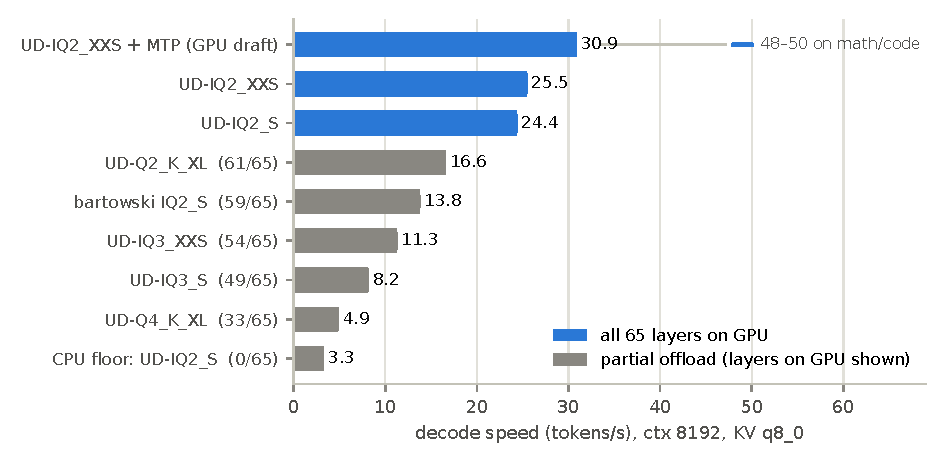
\includegraphics[width=\textwidth]{fig_ladder.pdf}
\caption{The measured speed ladder. Blue: all 65 layers GPU-resident; gray:
partial offload (GPU layer count in the label). The \q{UD-IQ2\_XXS}+MTP bar
shows prose decode; the whisker marks its measured 48--50\,tok/s on
math/code content (\S\ref{sec:mtp}). All base bars use the same
\q{llama-bench} tg128 protocol; the MTP annotations are separate server
measurements.}
\label{fig:ladder}
\end{figure}

Table~\ref{tab:phase1} and Figure~\ref{fig:ladder} give the matrix. The
full-residency boundary is the dominant feature; nominal labels and prompt
processing add two important qualifications.

\paragraph{For llama.cpp/GGUF, the full-GPU boundary lies between 7.8 and
9.2\,GiB in this run state.}
With the desktop session holding $\sim$900\,MiB, only the 6.8 and 7.8\,GiB
artifacts fit all 65 layers. Everything larger sheds layers to system RAM and
slows immediately. Within the GGUF ladder, footprint and consequent residency
are the first-order predictors of speed. This boundary is engine-specific:
ExLlamaV3 later fits a 9.50\,GiB EXL3 checkpoint (\S\ref{sec:exl3}).

\paragraph{The nominal quant label does not determine footprint or speed.}
Unsloth's \q{UD-IQ2\_S} (7.8\,GiB, 2.49 effective bpw) runs 24.4\,tok/s;
bartowski's \q{IQ2\_S} (9.6\,GiB, 3.06 effective bpw) runs 13.8\,tok/s. The
files share a nominal label but not a size, tensor allocation, or packaging:
the bartowski file also embeds MTP tensors. The observed speed difference is
consistent with full versus partial residency; it does not isolate a
quant-maker or allocation effect.

\paragraph{At 512 prompt tokens, GPU-heavy configurations ingest much faster
than they decode.} The controlled pp512 rates were 360--733\,tok/s, while the
CPU-only i-quant floor fell to 4.1\,tok/s. These short-context microbenchmarks
must not be extrapolated to 32K prompts; the deadline behavior in
\S\ref{sec:exl3} shows why.


\subsection{Offload Decay Follows a Two-Bandwidth Model}
\label{sec:offload}

\begin{figure}[t]
\centering
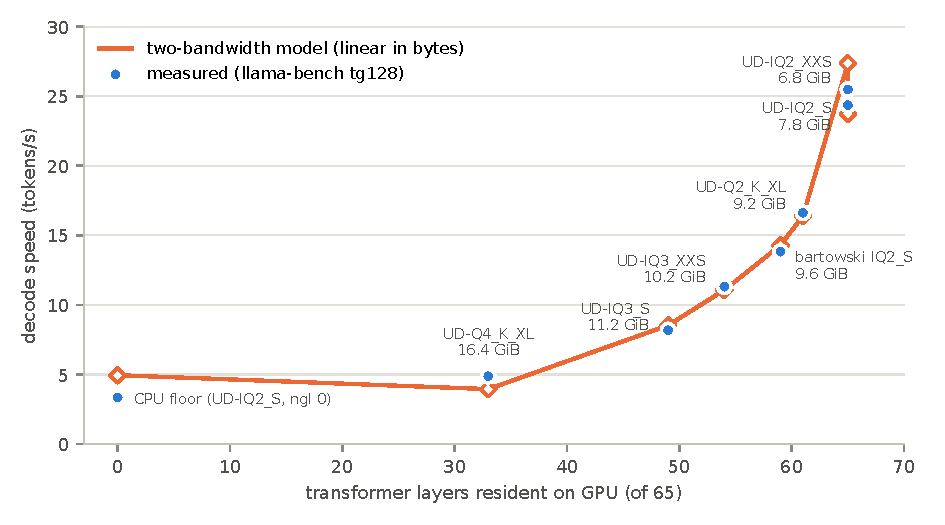
\includegraphics[width=\textwidth]{fig_offload.pdf}
\caption{Decode speed vs.\ GPU-resident layer count (blue, measured), with the
two-bandwidth model's per-config predictions (orange). The model, fitted for
relative error over all eight points, is
$1/\text{tok/s} = b_{\text{GPU}}/199\,\text{GB/s} +
b_{\text{CPU}}/41\,\text{GB/s}$ where $b$ are resident byte counts
(file bytes split proportionally to layers). The six non-extreme measured
states land within $\pm 8\%$; the two extremes' deviations are consistent with a
quant-family-dependent CPU term (i-quants dequantize expensively on CPU, so the ngl-0
floor runs $32\%$ below the pure-bandwidth prediction, while k-quant
\q{UD-Q4\_K\_XL} runs $24\%$ above it).}
\label{fig:offload}
\end{figure}

Figure~\ref{fig:offload} tests the bandwidth model of \S\ref{sec:hw} against
the matrix. Per-token time is linear in the two resident byte counts, with
fitted effective path bandwidths of \textbf{199\,GB/s} (GPU-resident bytes)
and \textbf{41\,GB/s} (CPU-resident bytes) --- a $4.9\times$ ratio, and the
reason each shed layer costs so much.
The fit's residual structure is itself informative: deviations concentrate
where CPU dequantization cost differs by quant family, i.e., the ``linear in
bytes'' rule needs a per-family CPU coefficient before it can be used
predictively across formats. For ranking configs on one family it is already
accurate to a few percent.


\subsection{MTP Benefit Depends on Workload and Placement}
\label{sec:mtp}

On the controlled prose prompt, the MTP draft head increased decode throughput by
21\% (25.5 $\rightarrow$ 30.9\,tok/s) at temperature 1.0 with the draft fully
on GPU, at a 41\% acceptance rate. During the MATH run, the same deployed
configuration produced 45--50 output tokens/s. That higher workload rate is
consistent with greater acceptance on structured text, but no draft-off run was
collected on the identical MATH prompts, so it is not a controlled 90\% MTP
effect. Likewise, the 9.6\,s mean GSM8K item time for
\q{UD-IQ2\_XXS}+MTP versus 17.7\,s for \q{UD-IQ2\_S} is a deployment
comparison, not an isolated MTP comparison: both the artifact and draft setting
change.

Two operational caveats. First, with the draft on CPU, MTP was a \emph{loss}
($-16\%$) or a wash in the controlled prose runs; these results should not be carried
over to other sampling regimes. Second, the draft's
VRAM cost is treacherous: $\sim$2.8\,GiB GPU-side when GPU-hosted, and still
$\sim$\textbf{1.2\,GiB} when nominally CPU-hosted (\q{-ngld 0}), because its
context and compute buffers allocate on the GPU regardless. This silently
crashed every tightly fitted mid-size config in our first sweep (the
``crashed'' rows of Table~\ref{tab:phase1}) until the harness guard learned to
account for it.

The result is therefore configuration-specific: MTP can help substantially
when the draft fits on GPU, but it is neither free in VRAM nor described by one
workload-independent speedup.



\subsection{Easy-Suite Accuracy Screen}
\label{sec:phase2}
\label{sec:phase2a}

\begin{table}[t]
\centering
\small
\caption{GSM8K ($n{=}50$) and HumanEval (executed, $n{=}20$) at
reasoning-effort medium, with Wilson 95\% CIs. Correct/min $=$ number of
successful items divided by summed logged HTTP-response wall time (local
post-response scoring excluded); compare only within a suite.}
\label{tab:phase2a}
\begin{tabular}{lrllrr}
\toprule
Config & tok/s & GSM8K & HumanEval & \multicolumn{2}{c}{correct/min} \\
 & & & & GSM8K & HE \\
\midrule
\q{UD-IQ2\_XXS}+MTP & 30.9 ($\approx$49 math) & 96\% [86.5, 98.9] & 80\% [58.4, 91.9] & \textbf{6.01} & 1.66 \\
\q{UD-IQ2\_S} & 24.4 & 94\% [83.8, 97.9] & \textbf{100\%} [83.9, 100] & 3.18 & \textbf{1.67} \\
\q{UD-Q2\_K\_XL} & 16.6 & 94\% [83.8, 97.9] & 100\% [83.9, 100] & 2.26 & 1.53 \\
\q{IQ2\_S} (bartowski) & 13.8 & 98\% [89.5, 99.6] & 95\% [76.4, 99.1] & 2.21 & 1.05 \\
\q{UD-IQ3\_XXS} & 11.3 & 96\% [86.5, 98.9] & 100\% [83.9, 100] & 1.65 & 0.92 \\
\q{UD-IQ3\_S} & 8.2 & 98\% [89.5, 99.6] & 100\% [83.9, 100] & 1.23 & 0.70 \\
\q{UD-Q4\_K\_XL} & 4.9 & 98\% [89.5, 99.6] & 100\% [83.9, 100] & 0.66 & 0.42 \\
\bottomrule
\end{tabular}
\end{table}

Table~\ref{tab:phase2a} has little resolution among the larger artifacts:
GSM8K estimates span 94--98\%, and HumanEval estimates span 95--100\% above
2.16 effective bpw. \q{UD-IQ2\_XXS} has the lowest HumanEval estimate (80\%),
but all intervals are wide. The practical difference is time. Across these two
suites, \q{UD-Q4\_K\_XL} used $4.6\times$ the pooled wall-clock of
\q{UD-IQ2\_S} ($7318\,\text{s}/1606\,\text{s}$) and recorded two additional
successes out of 70; no accuracy difference was resolved. Because these older
suites cluster near the top of their scales, the next experiments use the fixed MATH-25
subset and HumanEval+ to seek greater separation.


\subsection{MATH Answer-Parser Sensitivity}
\label{sec:artifact}

The original MATH parser scored \q{UD-IQ2\_S} at 14/25 and
\q{UD-IQ3\_XXS} at 22/25. Inspection of the saved responses found rejected
strings that differed from the reference in answer tags, math delimiters,
Unicode symbols, degree notation, brace shorthand, or an equation such as
\q{x=5} where the key contained \q{5}.

After inspecting those failures, we wrote a deterministic alternate
normalizer and applied it to every saved prediction. It accepts the declared
equivalences, leaves truncations wrong, and leaves mechanically unresolved
cases wrong. Because the rules were chosen post hoc, this score is not an
independent measure of mathematical correctness and does not replace the
original deployment parser. Table~\ref{tab:math25} and
Figure~\ref{fig:artifact} report both scores, with the rules and retained
per-item scoring records available for audit. No inference was rerun for this
analysis.

\begin{table}[t]
\centering
\small
\caption{MATH-25 ($n{=}25$, competition level 4--5): original parser score
vs.\ alternate-normalizer score, with the number of upgraded items
(value-equivalent under the alternate rules) and truncations (8K generation
budget exhausted; wrong under both scorers). Wilson 95\% CIs use the alternate
score. Reasoning-effort medium except where noted. Two \q{UD-Q4\_K\_XL} rows
lost their ground-truth field to a harness bug; the rescorer recovers them from
the dataset.}
\label{tab:math25}
\setlength{\tabcolsep}{5pt}
\begin{tabular}{lrrlcc}
\toprule
Config (eff.\ bpw) & Original & Alternate & CI (alternate) & Upgraded & Trunc. \\
\midrule
\q{UD-IQ2\_XXS}+MTP (2.16) & 12/25 & 16/25 (64\%) & [44.5, 79.8] & 4 & 3 \\
\q{UD-IQ2\_S} (2.49) & 14/25 & \textbf{23/25 (92\%)} & [75.0, 97.8] & \textbf{9} & 1 \\
\q{UD-IQ2\_S}, xhigh (2.49) & 17/25 & 21/25 (84\%) & [65.3, 93.6] & 4 & 4 \\
EXL3 2.0\,bpw (3.03) & 20/25 & \textbf{24/25 (96\%)} & [80.5, 99.3] & 4 & 1 \\
\q{IQ2\_S} bartowski (3.06) & 20/25 & 23/25 (92\%) & [75.0, 97.8] & 3 & 1 \\
\q{UD-IQ3\_XXS} (3.25) & 22/25 & \textbf{24/25 (96\%)} & [80.5, 99.3] & 2 & 0 \\
\q{UD-Q4\_K\_XL} (5.22) & 18/25 & 23/25 (92\%) & [75.0, 97.8] & 5 & 0 \\
\bottomrule
\end{tabular}
\end{table}

\begin{figure}[t]
\centering
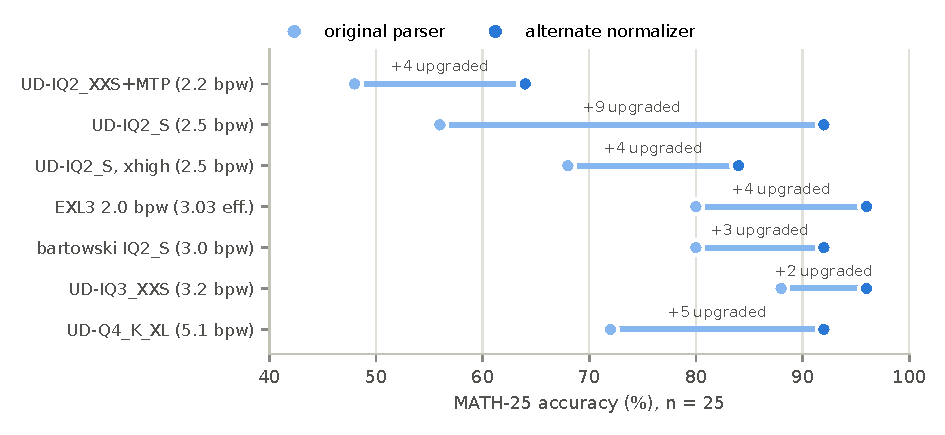
\includegraphics[width=\textwidth]{fig_artifact.pdf}
\caption{Original$\rightarrow$alternate score changes on MATH-25 ($n{=}25$).
The connector shows how many responses the post-hoc normalizer accepts that
the original parser rejected; both endpoints remain visible because the
rescore is not independent ground truth. The largest change is 9/25 at 2.49 effective bpw, versus
2/25 at 3.25 effective bpw.}
\label{fig:artifact}
\end{figure}

\paragraph{Accuracy across artifacts.}
Under the post-hoc normalizer, the estimates from 2.49 to 5.22 effective bpw
are 92--96\% and are not resolved from one another at this sample size. The
2.16-effective-bpw artifact scored 16/25, compared with 23/25 at 2.49 bpw on
the same items: seven successes favored the 2.49-bpw artifact and none favored
2.16 bpw (paired exact $p{=}0.016$, exploratory and uncorrected). No GGUF was
tested between 2.16 and 2.49 effective bpw, so the experiment identifies a
difference between these artifacts, not a universal threshold.

\paragraph{Parser sensitivity.}
For \q{UD-IQ2\_S}, the post-hoc normalizer accepted 9/25 responses rejected by
the original parser; for \q{UD-IQ3\_XXS}, it accepted 2/25. On the paired
items, seven changed only for IQ2\_S and none only for IQ3\_XXS (exact
$p{=}0.016$, exploratory and uncorrected). This establishes that parser
acceptance changed the apparent gap unevenly in these saved outputs. It does
not establish that every newly accepted response is semantically correct, or
that quantization generally harms answer formatting before reasoning.
Parser-compatible output remains a real deployment capability, so both scores
are retained.

\paragraph{Execution-scored code.} Generated code is
extracted from a fenced block and then executed, so it avoids symbolic-answer
normalization but still treats a missing/malformed code block as failure. We did
not post-hoc rescore those format failures; Table~\ref{tab:hard} reports the
end-to-end parser and test outcome as deployed.


\subsection{Hard-Suite Accuracy}
\label{sec:phase2b}

\begin{table}[t]
\centering
\small
\caption{Hard-suite summary (reasoning-effort medium). HumanEval+ is
execution-scored ($n{=}20$), Wilson 95\% CIs. Correct/min uses the
alternate MATH-25 score and each run's summed logged HTTP-response wall time;
post-response parsing and code execution are excluded.
The xhigh HumanEval+ entry is the truncation-free re-run
(\S\ref{sec:effort}).}
\label{tab:hard}
\setlength{\tabcolsep}{4pt}
\begin{tabular}{lllrr}
\toprule
Config (eff.\ bpw) & MATH-25 (alternate) & HumanEval+ & \multicolumn{2}{c}{correct/min} \\
 & & & math & HE+ \\
\midrule
\q{UD-IQ2\_XXS}+MTP (2.16) & 64\% [44.5, 79.8] & 70\% [48.1, 85.5] & 0.69 & 1.99 \\
\q{UD-IQ2\_S} (2.49) & 92\% [75.0, 97.8] & 90\% [69.9, 97.2] & 0.73 & 1.40 \\
\q{UD-IQ2\_S}, xhigh (2.49) & 84\% [65.3, 93.6] & 80\% [58.4, 91.9] & 0.37 & 0.73 \\
EXL3 2.0\,bpw (3.03) & \textbf{96\%} [80.5, 99.3] & 90\% [69.9, 97.2] & \textbf{0.83} & \textbf{2.27} \\
\q{IQ2\_S} bartowski (3.06) & 92\% [75.0, 97.8] & 90\% [69.9, 97.2] & 0.38 & 0.86 \\
\q{UD-IQ3\_XXS} (3.25) & \textbf{96\%} [80.5, 99.3] & 90\% [69.9, 97.2] & 0.33 & 0.73 \\
\q{UD-Q4\_K\_XL} (5.22) & 92\% [75.0, 97.8] & \textbf{95\%} [76.4, 99.1] & 0.19 & 0.43 \\
\bottomrule
\end{tabular}
\end{table}

Table~\ref{tab:hard} collects the hard suites. The 2.16-effective-bpw artifact
has the lowest point estimate on both: 16/25 alternate MATH and 14/20
HumanEval+, compared with 23/25 and 18/20 for the 2.49-bpw artifact. Because
every configuration saw the same items, paired tests are appropriate. The
MATH comparison has seven IQ2\_S-only successes and no IQ2\_XXS-only successes
(exact two-sided $p{=}0.016$); HumanEval+ has four and zero, respectively
($p{=}0.125$). Thus these data resolve the MATH loss but not the code-suite
difference. We do not pool the two suites into a single significance test.

Above 2.16 effective bpw, alternate MATH estimates are 92--96\% and HumanEval+
estimates are 90--95\%; no difference is resolved at these sample sizes. That
is evidence for a plateau within this experiment, not proof that the artifacts
or formats are equivalent. It also reinforces why nominal ``2-bit'' is too
coarse a label: the evaluated files bearing it span 2.16--3.06 effective bpw
and produced materially different hard-suite point estimates.


\subsection{Matched-Footprint Deployment Comparison}
\label{sec:exl3}

The EXL3 checkpoint is labeled 2.0\,bpw, but its 9.50\,GiB weight-file total is
\textbf{3.03 effective bpw}: the transformer weights target roughly 2\,bpw,
while the output head is 3-bit and other tensors are wider. It therefore is
not a footprint-matched comparison with the 6.77\,GiB, 2.16-effective-bpw
GGUF. Crediting their quality difference to trellis coding would confound
method with 40\% more effective bits.

The direct footprint control is bartowski \q{IQ2\_S}: 9.59\,GiB and 3.06
effective bpw. On identical hard-suite subsets, EXL3 scored 24/25 versus 23/25
on alternate MATH and both scored 18/20 on HumanEval+. These small samples do
not resolve a quality difference. They do expose a deployment difference: the
EXL3--ExLlamaV3 stack was fully GPU-resident, whereas the
bartowski-GGUF--llama.cpp stack offloaded six of 65 units. From the server logs
on these same workloads,
token-weighted generation throughput was 22.4 versus 13.7\,tok/s on MATH
($1.64\times$) and 30.7 versus 13.8\,tok/s on HumanEval+ ($2.22\times$).
The rate varies with output length and workload, so we use the MATH result as
the headline comparison: \textbf{at matched footprint, the fully resident
EXL3 deployment generated $1.6\times$ faster, and the available hard-suite
samples did not resolve a score difference.}

The other measured comparisons clarify what this result does and does not
identify:

\begin{itemize}
  \item At similar effective bpw, EXL3 (3.03) and \q{UD-IQ3\_XXS} (3.25)
  both scored 24/25 on alternate MATH and 18/20 on HumanEval+. We measured no
  quality-per-effective-bit advantage for either artifact at this point.
  \item Against \q{UD-IQ2\_XXS} (2.16), EXL3 has higher point scores but also
  a 2.73\,GiB larger file. This experiment cannot locate a trellis-specific
  quality boundary near 2.2 effective bpw.
\end{itemize}

This is the concrete sense in which the 12\,GB system exceeded a naive
capacity-based expectation: a 9.50\,GiB checkpoint remained resident and ran
at useful speed, while a nearly identical-size GGUF offloaded weights to RAM.
Because format and engine changed together, the experiment compares complete
deployments and cannot attribute the difference to trellis coding alone.

\begin{table}[t]
\centering
\small
\caption{Selected-deployment validation. MMLU used the same fixed 200-item,
57-subject-stratified subset; CIs are Wilson 95\%. Correct/min uses logged
HTTP-response wall time (post-response scoring excluded). Needle reports
probes completed correctly
before the client exhausted two 600-s HTTP attempts (one automatic retry),
not pure retrieval accuracy.}
\label{tab:validation}
\setlength{\tabcolsep}{5pt}
\begin{tabular}{lrrrl}
\toprule
Config & MMLU & Mean wall/item & Correct/min & Needle deadline success \\
\midrule
\q{UD-IQ2\_S} & 175/200, 87.5\% [82.2, 91.4] & 36.41\,s & 1.44 & 4/6 [30.0, 90.3] \\
EXL3 2.0\,bpw & 182/200, 91.0\% [86.2, 94.2] & 25.42\,s & 2.15 & 6/6 [61.0, 100] \\
\bottomrule
\end{tabular}
\end{table}

On paired MMLU items, both were correct on 171, only \q{UD-IQ2\_S} on four,
only EXL3 on 11, and neither on 14 (exact two-sided McNemar $p{=}0.119$).
The 3.5-point estimate therefore does not resolve a quality difference, while
EXL3 returned more correct items per minute. On the needle probes,
\q{UD-IQ2\_S} answered all four 8K/16K contexts but its two 32K items produced
no answer after two 600-s HTTP attempts each (one automatic retry after a
2-s delay, or about 1,202\,s total per item); EXL3 completed all six. The
4/6 versus 6/6 count measures completion under this client policy and includes
a large prompt-processing difference, so it must not be read as two wrong
retrieval answers.


\subsection{Reasoning-Effort Check}
\label{sec:effort}

Qwen3.8's chat template exposes a \q{reasoning\_effort} dial. For
\q{UD-IQ2\_S}, xhigh produced no observed benefit. On MATH-25 it scored
21/25 (84\%) under the alternate normalizer versus 23/25 (92\%) at medium,
with four rather than one 8K truncations. Mean wall time rose from 75.89 to
134.44\,s per item ($1.77\times$). On HumanEval+, an initial xhigh run was
truncation-confounded; the 8K-budget re-run removed truncations and scored
16/20 (80\%) versus 18/20 (90\%) at medium. Neither accuracy difference is
resolved at this sample size. The useful conclusion is narrower: xhigh was
slower and did not improve either point estimate in these runs, so medium is
the better measured setting for this deployment. This is not evidence that
additional reasoning effort is generally harmful.



\subsection{Correct Responses per Minute at Fixed VRAM}
\label{sec:metric}

\begin{figure}[t]
\centering
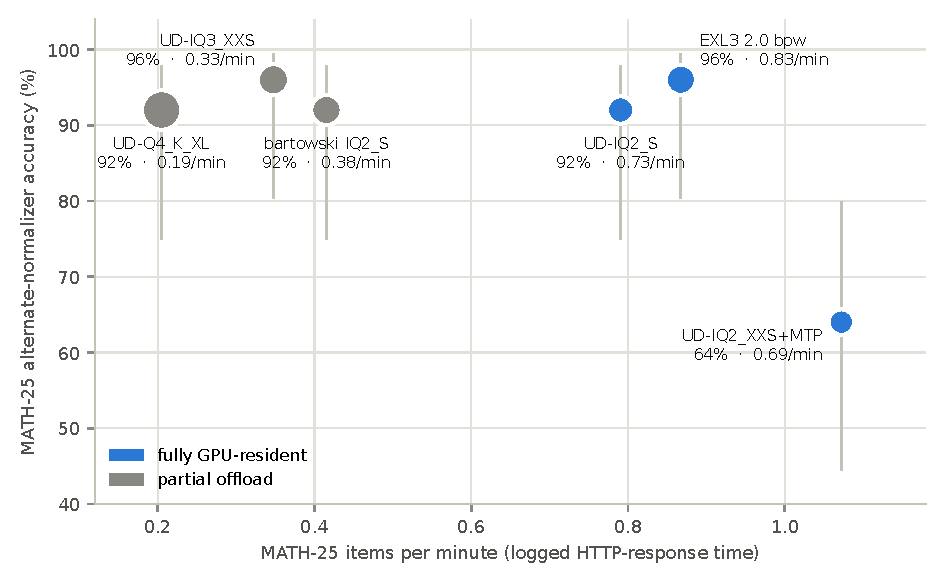
\includegraphics[width=\textwidth]{fig_frontier.pdf}
\caption{MATH-25 point estimates using logged HTTP-response time.
$x$: benchmark items completed per minute, whether correct or not; $y$:
alternate-normalizer accuracy with Wilson 95\% intervals; point area
$\propto$ file GiB. Their product is correct responses per minute. Colors
encode the measured residency state. The vertical intervals overlap widely;
the plot compares observed deployment rates and does not establish quality
dominance.}
\label{fig:frontier}
\end{figure}

For a fixed suite, correct responses per minute is the number scored correct
divided by summed per-item HTTP-response wall time. The timer includes prompt
processing, generation, retries, and request overhead, but stops before local
post-response parsing or code execution. It answers a deployment question---
how many successful model responses this machine returned per minute---without
pretending that a correct MATH item and a correct HumanEval+ item have the same
value. We therefore compare it only within a suite and always print the
underlying accuracy beside it.

The response-time view in Figure~\ref{fig:frontier} avoids the cross-engine
token/s problem: it prices prompt processing, generation length, retries,
request overhead, MTP, and offload as logged. It does not price local scoring.
On MATH-25, EXL3 has the highest observed
correct/min (0.83), followed by fully resident \q{UD-IQ2\_S} (0.73) and the
faster but less accurate \q{UD-IQ2\_XXS}+MTP (0.69). The partial-offload
artifacts range from 0.19 to 0.38. On HumanEval+, EXL3 has the highest
observed rate at 2.27, followed by the faster but lower-scoring
\q{UD-IQ2\_XXS}+MTP at 1.99 and \q{UD-IQ2\_S} at 1.40. These are efficiency
estimates on the observed subsets, not statistically distinct quality
rankings or a recommendation that ignores error cost.


\section{Discussion}
\label{sec:discussion}

\subsection{Deployment Recommendations}

For this machine, the measurements support distinct deployment choices.
Extrapolation to
other 12\,GB systems requires repeating the fit search because desktop VRAM,
engine buffers, and memory bandwidth change the boundary.

\begin{enumerate}
  \item \textbf{Default when the ExLlamaV3 stack is suitable: EXL3
  2.0\,bpw (3.03 effective).} It has the highest measured hard-suite
  correct/min and, among the two configurations selected for validation, the highest MMLU
  correct/min, with no resolved quality difference from the larger tested
  anchors. Its speed advantage is workload-dependent, and this run did not
  configure MTP or vision.
  \item \textbf{GGUF all-rounder: \q{UD-IQ2\_S}.} It remains fully resident,
  scored 92\%/90\% on the hard suites, and uses the llama.cpp/GGUF stack. The
  separate unsloth MTP draft did not fit in the measured desktop run state.
  \item \textbf{Maximum throughput when errors are cheaper:
  \q{UD-IQ2\_XXS}+MTP.} It delivered the fastest measured generation and
  6.01 correct GSM8K items/min, but its 64\% alternate MATH and 70\%
  HumanEval+ estimates were lower than the resident alternatives. It is not
  the recommendation for correctness-sensitive work.
\end{enumerate}


\subsection{Research Directions}

These measurements motivate a broader systems hypothesis: under a fixed VRAM
budget, useful single-stream throughput is often maximized by a deployment
that sits above the task-accuracy loss boundary but below the engine's
offload boundary. The present experiment establishes one instance, not a
general law. Testing the hypothesis requires repeating the same fit--speed--
accuracy map across models, engines, 8/12/16/24\,GB memory budgets, context
lengths, and power limits.

The highest-priority quality extension is a bf16, Q8, or hosted reference run
on hardware large enough to hold it. That would determine how much accuracy
all tested 12\,GB deployments lose relative to the original model; the current
Q4 anchor only supports comparisons within this experiment. Denser sampling
between 2.16 and 2.49 effective bpw, larger hard-task sets, and repeated
generations would test whether the observed GGUF drop is stable.

A method-level EXL3 claim would require tighter controls over tensor
precision, packaged components, kernels, and memory allocation, ideally with
one engine supporting both representations. The MATH audit can be strengthened
without rerunning inference: an independent, preregistered human or
computer-algebra review can rescore the archived predicted-answer fields. New inference
runs would be needed to estimate run-to-run variability or test whether
parser compatibility changes systematically with quantization.

\section{Limitations and Threats to Validity}
\label{sec:limitations}

\begin{itemize}
  \item \textbf{No unquantized quality reference.} We did not evaluate bf16,
  Q8, or the hosted model. Comparisons to \q{UD-Q4\_K\_XL} rank only the
  tested artifacts and do not establish parity with the original model.
  \item \textbf{Limited statistical power.} MATH-25 and HumanEval+ contain
  only 25 and 20 fixed items. Their Wilson intervals are wide; a non-significant
  comparison is not evidence of equality. MMLU is larger but tests a different
  capability mix. No correction was applied across the exploratory paired
  comparisons.
  \item \textbf{One stochastic sample.} Each item was generated once at
  temperature 1.0. The intervals quantify item sampling only, not variation
  across repeated generations.
  \item \textbf{Post-hoc alternate scoring.} The MATH normalizer was written
  after failures were inspected. Publishing its rules, retained per-item
  scoring records, original scores, and alternate scores makes the judgment
  auditable but does not make
  it independent or pre-registered.
  \item \textbf{Deployment, not method isolation.} The EXL3--GGUF comparison
  changes format, artifact, kernels, memory allocation, and engine together.
  It supports a choice between the tested deployments, not a causal claim
  about trellis coding.
  \item \textbf{Speed protocols.} The GGUF ladder uses controlled tg128 runs;
  no matching EXL3 microbenchmark was collected. Cross-engine ratios in
  \S\ref{sec:exl3} instead use engine-reported generation metrics on the same
  evaluation workloads. Correct/min uses logged HTTP-response wall time and is
  the more comparable deployment measure; it excludes local scoring time.
  \item \textbf{Scope and provenance.} Results come from one model, laptop,
  run state, and set of artifacts downloaded on one date. File sizes identify
  the local artifacts. Upstream revisions were recovered from the local cache
  after the campaign rather than emitted into the measurement logs at run
  time; the release records those revisions together with the exact file
  SHA-256 values. The 80\,W power limit is not an energy measurement, and no
  sustained thermal or per-watt conclusion is reported.
  \item \textbf{Long-context timeout contamination.} The two failed 32K
  \q{UD-IQ2\_S}+llama.cpp probes exhausted both 600-s HTTP attempts without
  returning an answer, so the needle comparison combines prompt-processing
  speed with retrieval behavior.
\end{itemize}



\section{Related Work}
\label{sec:related}

\textbf{Quantization methods.} This work evaluates existing post-training
quantization rather than introducing a method: GGUF k/i-quants in llama.cpp
\citep{gerganov2023llamacpp}, dynamic mixed-tensor GGUF recipes
\citep{unsloth2026dynamic}, and EXL3 \citep{turboderp2025exllamav3}, whose
trellis construction builds on QTIP \citep{tseng2024qtip}. GPTQ (published at
ICLR as OPTQ)
\citep{frantar2022gptq}, AWQ \citep{lin2023awq}, and ParetoQ
\citep{liu2025paretoq} provide broader calibration and low-bit scaling context.
Our effective-bpw accounting is a deployment-footprint measure, not a new
quantization metric.

\textbf{Post-freeze update (checked 2026-08-29).}
On 2026-08-28, after our 2026-08-25 artifact freeze, ISTA-DASLab released
Qwen3.8-27B checkpoints that use GSQ for low-bit scalar quantization and RCO
for per-tensor GGUF-type assignment under a file-size budget
\citep{dadgarnia2026gsq,helcig2026rco,istadaslab2026qwen38gsqrco}. They are
standard GGUF files, not a GSQ/RCO-specific runtime modification; we did not
evaluate their quality, residency, or correct/min on this system.

\textbf{Evaluation and answer parsing.} Prior work shows that aggregate task accuracy
can conceal important changes under quantization \citep{dutta2024accuracy},
and low-bit mathematical reasoning has been studied through process and error
taxonomies \citep{quantreasoning2025,extremelowbit2026}. Separately, structured
output research distinguishes semantic correctness from machine usability
\citep{correctnotusable2026}, while evaluation scaffolding can materially alter
measured outcomes \citep{scaffolding2026}. Task difficulty and instruction
following also interact with quantization \citep{quantinstruct2024}. Our
MATH audit is a small, concrete instance of these broader warnings: a
post-hoc alternate normalizer changed the apparent low-bit gap, so the
original-parser and post-hoc-normalized scores must remain visible. Community measurements that report strict or
machine-usable output rates provide a related operational view
\citep{strix2026}.

\textbf{Extreme-low-bit and cross-format comparisons.} Bielik-Q2-Sharp
compares six academic extreme-2-bit methods on an 11B Polish model and finds
that rankings depend on method and summary metric \citep{bielik2026q2sharp}.
Broader unified GGUF evaluation reports FP16, size, perplexity, throughput, and
standard downstream tasks on Llama-3.1-8B \citep{kurt2026whichquant}; a
contemporaneous Qwen3.8-27B study compares bf16 through 1-bit GGUFs on larger
datacenter GPUs \citep{migdal2026qwen38}. Those studies provide wider precision
or task coverage; the present question is the realized 12\,GB deployment
boundary.
EXL3's documentation reports its own quality curves
\citep{turboderp2025exllamav3}; an earlier matched-bpw community comparison
reported lower MMLU for lower-bpw EXL2 variants than for GGUF at matched
quantized-layer bpw on Llama~3 \citep{mattc1llama3}. Our data should not be
read as a method-level reversal of either result. At roughly 3 effective bpw we
resolve no hard-suite quality difference; the contribution is a matched-file-
footprint deployment comparison in which the EXL3 artifact remains resident
and the GGUF control does not.

\textbf{Local inference under resource constraints.} Bench360 evaluates
quality, latency, energy, and Pareto tradeoffs under a fixed 24\,GB budget
\citep{bench360}; other work studies accuracy--performance tradeoffs on server
GPUs \citep{kurtic2024bf16}, joint performance, energy, and quality under
online GPU serving \citep{qmeter2025}, and various combinations of latency,
quality, and energy on mobile, edge, or private-server systems
\citep{sustainableedge2025,palmbench2024,privateserver2025}. Silicon Showdown describes the consumer ``VRAM wall'' and
the throughput cost of CPU offload \citep{javat2026siliconshowdown}, while
pipelined sub-layer sharding targets that cost with a new client inference
system \citep{ukarande2026vram}.

Most directly, Moreira reports Qwen3.8-27B on a 12\,GB RTX~4070~Ti: a fully
resident IQ2 configuration generated at 43.643 tokens/s versus 5.977 for a
partially offloaded IQ4\_XS, while a 24-item custom suite favored IQ4\_XS
13--9 without resolving the paired difference \citep{moreira2026qwen38}.
Its desktop hardware, artifact, runtime, context, and speed protocol differ
from ours, so those absolute rates are prior evidence about the fit--offload
trade rather than a throughput baseline for this study.
Thus our study is not the first task-level fit-versus-offload measurement for
this model and memory class. It contributes an independent 80\,W laptop
characterization with standard task families, effective-footprint and
engine-residency accounting, a matched-footprint EXL3/GGUF deployment pair,
and an explicit parser audit. Correct/min is a descriptive within-suite
task-goodput rate, not a proposed universal or novel benchmark.

Our MTP measurements are an instance of speculative decoding
\citep{leviathan2022speculative,chen2023speculative}; they do not evaluate
speculative-decoding algorithms themselves.


\section{Artifact Availability and Reproducibility}
\label{sec:repro}

Every reported result traces to archived JSONL data alongside the harness:
\begin{itemize}
  \item fit searches, \q{llama-bench} results, timings, and VRAM peaks in
  \path{testsuite/results/phase1.jsonl};
  \item per-suite summaries in
  \path{testsuite/evals/results/summary.jsonl}; and
  \item per-item JSONL scoring records in each retained configuration's
  results directory, including predicted and expected answer fields and the
  final 200 characters of each saved response where applicable.
\end{itemize}
The alternate MATH-25 numbers come from the deterministic $\sim$50-line
\path{testsuite/evals/rescore_math25.py}; every rule is listed in
\S\ref{sec:artifact}. Figures are generated directly from these logs by
\path{paper/scripts/make_figures.py}. Engine server logs preserve the per-request
metrics used for the matched-workload comparison.

Software: llama.cpp master \q{b1-1729ed5}, CUDA 12.6.3 (user-local
toolchain), SM 8.9, flash-attn on; ExLlamaV3 1.4.3 under TabbyAPI
(\q{max\_seq\_len} 16384 for the main hard suites and 36864 for validation).
Artifacts: unsloth \q{Qwen3.8-27B-GGUF} UD tier,
bartowski \q{Qwen3.8-27B-GGUF} \q{IQ2\_S}, turboderp EXL3 \q{SC\_2.00bpw\_H3}
all downloaded 2026-08-25. File sizes in Table~\ref{tab:artifacts} identify
the local artifacts; the release manifest records every tested upstream
revision, filename, byte count, and SHA-256. Evaluation ran through each
engine's OpenAI-compatible endpoint; \q{reasoning\_effort} was passed per
request via \q{chat\_template\_kwargs}. Harness safety rules (VRAM fit guard
including the 1.2\,GiB \q{-ngld 0} draft-buffer correction, mmap-backed CPU
weights, one model process at a time) are documented in the harness and were
calibrated against the measured peaks in Table~\ref{tab:phase1}.

The public artifact should be used in two modes: an analysis-only path that
rebuilds tables and figures from archived logs without launching inference,
and a prospective replication path that downloads the pinned model artifacts
and reruns the GPU harness. The accompanying artifact includes a paper-specific README,
environment and hardware requirements, model revisions and checksums, concrete
setup and launch commands, expected outputs, and an immutable tag or archive
identifier. The version-of-record compendium is archived at
\href{https://doi.org/10.5281/zenodo.22166977}{doi:10.5281/zenodo.22166977};
the matching tagged source and results tree is
\url{https://github.com/matthematics1137/research-artifacts/tree/qwen38-27b-12gb-v1.0.0/papers/2026-qwen38-27b-12gb}.
The ML-facing result dataset is
\url{https://huggingface.co/datasets/mv1137/qwen38-27b-12gb-results}.
Full response transcripts were not retained: the per-item files contain scoring fields and
short answer excerpts. The Q4 easy-suite runs also lack per-item GSM8K and
HumanEval files and are supported only by their frozen aggregate summary rows.
We preserve these gaps rather than reconstructing records after the fact.


\section{Conclusion}

On the tested 12\,GB laptop, the best measured way to run Qwen3.8-27B was not
to load the largest artifact possible and accept CPU offload. Fully resident
GGUFs decoded at 24--25 tokens/s, while progressively offloaded GGUFs fell to
16.6--4.9 tokens/s. A 9.50\,GiB EXL3 checkpoint remained resident under
ExLlamaV3; compared with a 9.59\,GiB GGUF under llama.cpp, it generated
$1.6\times$ faster on MATH, had no hard-suite score difference resolved at the
available sample sizes, and produced the highest observed correct responses
per minute on MATH and HumanEval+.

The practical result is that this 12\,GB system ran a 27.4B model without the
repeated RAM weight reads that dominated the larger GGUF deployments. Finding
that operating point required the actual checkpoint footprint, engine memory
behavior, GPU residency, response time, and answer parser; the advertised bit
label alone was insufficient. This experiment does not establish parity with
bf16 or Q8, a universal optimum, or a trellis-specific advantage. Broader
claims require larger repeated evaluations, an unquantized or near-lossless
reference, and replication across models, engines, and memory budgets.

\medskip
\noindent\textbf{AI assistance.} Claude (Anthropic) and Codex (OpenAI) assisted
with evaluation-harness development, experiment execution, evidence auditing,
analysis and figure code, and manuscript drafting and revision. Matthew
Schwartz directed the work, reviewed and verified the retained outputs against
the archived evidence and cited sources, edited the manuscript, and takes full
responsibility for the methods, results, interpretation, citations, and
released artifacts.

\bibliographystyle{unsrtnat}
\bibliography{references}

% ===========================================================================

\end{document}
